

\clearpage
\thispagestyle{empty}

\vspace*{\fill}
\begin{center}
	{\Huge\bfseries Examen CEPREUNA 2024-I Primera Etapa}
\end{center}
\vspace*{\fill}

\clearpage

\section*{Área: Ingenierías}


\subsection*{Aritmética}

\begin{enumerate}
	
	
	
	% --- Pregunta 1 ---
	\item Siendo $A = \{ 1, 1, \{1\}, \emptyset \}$, determinar el valor de verdad de las siguientes proposiciones:
	\begin{itemize}
		\item[I.] $P(A)$ tiene 4 elementos
		\item[II.] $\{\emptyset\} \subset P(A)$
		\item[III.] $\{\emptyset\} \in P(A)$
		\item[IV.] $\emptyset \in P(P(A))$
	\end{itemize}
	\begin{enumerate}[label=\alph*)]
		\item FVVV
		\item VVVV
		\item VVVF
		\item VVFF
		\item FVVF
	\end{enumerate}
	\textbf{Respuesta correcta:} a) 
	
	\vspace{2mm}
	\textbf{Solucionario:}\\
	$A = \{1, \{1\}, \emptyset\}$, $P(A) = \{\{1\}, \{\{1\}\}, \{\emptyset\}, \dots \}$.\\
	$n[P(A)] = 2^{n(A)} = 2^3 = 8$\\
	\\
	$\{\emptyset\} \subset P(A) \quad (V)$ ya que $\emptyset \in P(A)$\\
	$\{\emptyset\} \in P(A) \quad (V)$\\
	$\emptyset \in P(P(A)) \quad (V)$
	
	\vspace{6mm}
	
	% --- Pregunta 2 ---
	\item Determine el equivalente a la proposición: "es falso que, hace calor y no estudié"
	\begin{enumerate}[label=\alph*)]
		\item hace calor o no estudié.
		\item No hace calor o no estudié.
		\item Hace calor y no estudié.
		\item Si hace calor entonces estudié.
		\item Estudio dado que hace calor.
	\end{enumerate}
	\textbf{Respuesta correcta:} e)
	
	\vspace{2mm}
	\textbf{Solucionario:}\\
	$p$: hace calor. $\quad q$: estudia\\
	$\sim (p \wedge \sim q)$\\
	ley de morgan.\\
	$\sim p \vee q \equiv p \rightarrow q$\\
	$\therefore$ Estudio dado que hace calor.
	
	\vspace{6mm}
	
	% --- Pregunta 3 ---
	\item Ocho obreros realizan una obra en 20 días. Después de 5 días de trabajo, se retiran 3 obreros. ¿Con cuántos días de atraso se termina la obra?
	\begin{enumerate}[label=\alph*)]
		\item 24 días
		\item 25 días
		\item 16 días
		\item 12 días
		\item 9 días
	\end{enumerate}
	\textbf{Respuesta correcta:} e)
	
	\vspace{2mm}
	\textbf{Solucionario:}\\
	Como después de 5 días se retiraron 3 obreros $\Rightarrow 8$ obreros lo harán 15 días\\
	\begin{tabular}{|c|c|}
		\hline
		Antes & Ahora \\
		8 obreros & 5 obreros \\
		15 días & X días \\
		\hline
	\end{tabular} la misma cantidad de obra para los dos grupos.\\
	\\
	Lo que falta lo hacen:\\
	\begin{tabular}{lcc}
		& obreros & tiempo \\
		antes & 8       & 15 \\
		ahora & 5       & X
	\end{tabular}\\
	\\
	$X = \frac{(15)(8)}{5} = 24$ días.\\
	$\leadsto$ retraso $= 24 - 15 = 9$ días //
	
	\vspace{6mm}
	
	% --- Pregunta 4 ---
	\item A una fiesta de promoción asistieron 140 alumnos entre hombres y mujeres. Por cada 3 mujeres hay 4 hombres. Si se retiran 20 parejas, ¿Cuál es la razón entre el número de mujeres y el número de hombres que se quedan en la fiesta?
	\begin{enumerate}[label=\alph*)]
		\item 3/4
		\item 2/3
		\item 3/2
		\item 1/3
		\item 4/3
	\end{enumerate}
	\textbf{Respuesta correcta:} b)
	
	\vspace{2mm}
	\textbf{Solucionario:}\\
	Sean $H_0$ y $M_0$ el número de hombres y mujeres al iniciarse la fiesta. Por condición sabemos:\\
	$H_0 + M_0 = 140 \quad \dots (1)$\\
	$\frac{M_0}{H_0} = \frac{3}{4} \Rightarrow \left. \begin{array}{l} M_0 = 3K \\ H_0 = 4K \end{array} \right\} (II)$\\
	Remplazando (ii) en (1):\\
	$4K + 3K = 140 \Rightarrow K = 20$\\
	$\Rightarrow M_0 = 60$ y $H_0 = 80$\\
	Como se retiran 20 parejas implica 20 hombres y 20 mujeres. Así la nueva cantidad será:\\
	$H = 80 - 20 = 60$\\
	$M = 60 - 20 = 40$\\
	$\frac{M}{H} = \frac{40}{60} = \frac{2}{3} $
	
	
	\vspace{6mm}
	
\end{enumerate}


\subsection*{Álgebra}

\begin{enumerate}
	
	% --- Pregunta 5 (Libro de Omar) ---
	\item Omar lee un libro de la siguiente manera: el primer día lee una página, el segundo día lee el doble del primer día, el tercer día lee el doble del día anterior y así sucesivamente hasta que el último día lee 128 páginas. ¿Durante cuántos días Omar estuvo leyendo el libro?
	\begin{enumerate}[label=\alph*)]
		\item 6 días
		\item 7 días
		\item 8 días
		\item 9 días
		\item 10 días
	\end{enumerate}
	\textbf{Respuesta correcta:} c)
	
	\vspace{2mm}
	\textbf{Solucionario:}\\
	\begin{tabular}{ll}
		Días & \# de págs. \\
		1 & $1 = 2^0$ \\
		2 & $2 = 2^1$ \\
		3 & $4 = 2^2$ \\
		\vdots & \vdots \\
		x días & $2^{x-1}$
	\end{tabular} \\
	\\
	$\therefore 2^{x-1} = 128 = 2^7 \Rightarrow x = 8$ días
	
	\vspace{6mm}
	
	% --- Pregunta 6 (Polinomio de Ruffini/Horner) ---
	\item Dado el polinomio $P(x) = x^4 + \sqrt{3}x^3 - x^2 + \sqrt{3}x + 6$, halle $P(1-\sqrt{3})$.
	\begin{enumerate}[label=\alph*)]
		\item $9 - \sqrt{3}$
		\item $3 - 3\sqrt{3}$
		\item $9 - 3\sqrt{3}$
		\item $6 + \sqrt{3}$
		\item 9
	\end{enumerate}
	\textbf{Respuesta correcta:} c)
	
	\vspace{2mm}
	\textbf{Solucionario:}\\
	\begin{tabular}{r|rrrr|c}
		& 1 & $\sqrt{3}$ & $-1$ & $\sqrt{3}$ & 6 \\
		$1-\sqrt{3}$ & $\downarrow$ & $1-\sqrt{3}$ & $1-\sqrt{3}$ & $\sqrt{3}+3$ & $3-3\sqrt{3}$ \\ \hline
		& 1 & 1 & $-\sqrt{3}$ & 3 & \fbox{$9-3\sqrt{3}$}
	\end{tabular} \\
	\\
	$\therefore P(1-\sqrt{3}) = 9-3\sqrt{3}$
	
	\vspace{6mm}
	
	% --- Pregunta 7 (Dominio de funciones compuestas) ---
	\item Dadas las funciones $f(x) = \sqrt{1-x}$ y $g(x) = \sqrt{4-x}$. Halle el dominio de la función compuesta $f \circ g$.
	\begin{enumerate}[label=\alph*)]
		\item $\langle3,4\rangle$
		\item $[3, 4]$
		\item $\langle3, 4]$
		\item $[3, 4\rangle$
		\item $\langle -\infty , 4]$
	\end{enumerate}
	\textbf{Respuesta correcta:} b)
	
	\vspace{2mm}
	\textbf{Solucionario:}\\
	$D_{f \circ g} = \{ x \in \mathbb{R} \mid x \in D_g \wedge g(x) \in D_f \}$ \\
	$D_f: 1-x \geq 0 \rightarrow x \leq 1$ \\
	$D_g: 4-x \geq 0 \rightarrow x \leq 4$ \\
	\\
	$x \leq 4 \wedge 0 \leq \sqrt{4-x} \leq 1$ \\
	$0 \leq 4-x \leq 1$ \\
	$-4 \leq -x \leq -3$ \\
	$3 \leq x \leq 4$ \\
	\\
	$\therefore D_{f \circ g} = [3, 4]$
	
	\vspace{6mm}
	
	% --- Pregunta 8 (Cociente notable) ---
	\item En el desarrollo del cociente notable dado, indique el número de términos.
	$$\frac{a^{5p-5} - b^{4p-4}}{a^{p-4} - b^{p-5}}$$
	\begin{enumerate}[label=\alph*)]
		\item 7
		\item 8
		\item 9
		\item 10
		\item 11	
	\end{enumerate}
	\textbf{Respuesta correcta:} b)
	
	\vspace{2mm}
	\textbf{Solucionario:}\\
	$\frac{5p-5}{p-4} = \frac{4p-4}{p-5}$ por ser C.N. \\
	$5(p-1)(p-5) = 4(p-1)(p-4)$ \\
	$5p - 25 = 4p - 16$ \\
	$p = 9$ \\
	\\
	$\therefore \# \text{términos} = \frac{5(9)-5}{9-4} = \frac{40}{5} = 8$
	
	\vspace{6mm}
	
\end{enumerate}



\subsection*{Geometria}

\begin{enumerate}

\item En un terreno de cultivo de forma rectangular, se toma una porción de forma triangular para la siembra de maíz. En dicha porción, una de sus esquinas es el centro del terreno de cultivo. ¿Cuál es el ancho del terreno si su diagonal es 600 m?

% (Dejar aquí el gráfico)
	\begin{center}
	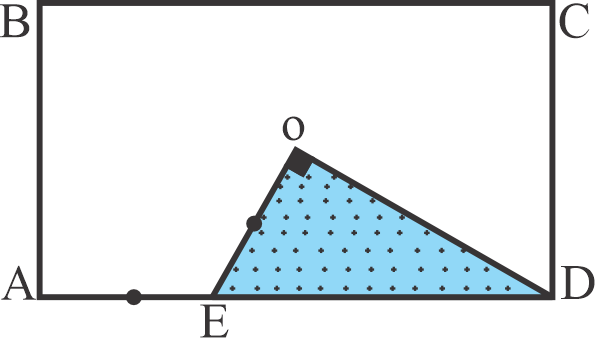
\includegraphics[width=4.5cm]{imagenes/CEPRE-UNA2024-I/etapa1/ing/geo1c24-I.png}
	\end{center}

\begin{enumerate}[label=\alph*)]
	\item $250\,m$
	\item $200\,m$
	\item $300\,m$
	\item $275\,m$
	\item $325\,m$
\end{enumerate}

\textbf{Respuesta correcta:} c)

\vspace{2mm}
\textbf{Solucionario:}\\



	\begin{center}
	\begin{minipage}{0.45\textwidth}
		Al trazar sus diagonales, se cumple:\\
		$OA = OB = OC = OD = 300\,m$\\
		$m\angle OAD = m\angle ODA = \theta$\\
		$\triangle AEO$: isosceles\\
		$m\angle EAO = m\angle EOA = \theta \Rightarrow m\angle OED = 2\theta$\\
		$\triangle EOD$: $3\theta = 90^\circ \Rightarrow \theta = 30^\circ$\\
		$\triangle OHB$: Notable $(30^\circ; 60^\circ)$\\
		$BH = HA = 150\,m$\\
		$\therefore AB = 300\,m$
		
		\vspace{6mm}
	\end{minipage}
	\hfill
	\begin{minipage}{0.45\textwidth}
		\centering
		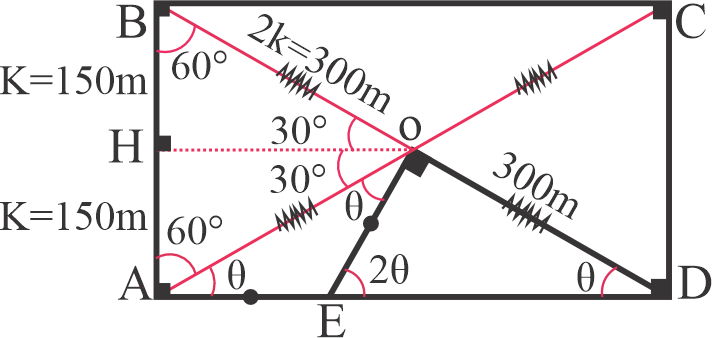
\includegraphics[width=5.5cm]{imagenes/CEPRE-UNA2024-I/etapa1/ing/geo1c24-Ir.png}
	\end{minipage}
\end{center}
\vspace{6mm}



\item Un poste está sujeto al suelo con dos cables tensores. Si el cable de mayor longitud con el poste forma un ángulo de $30^\circ$, calcule la medida del ángulo formado por los dos cables.

\begin{center}
	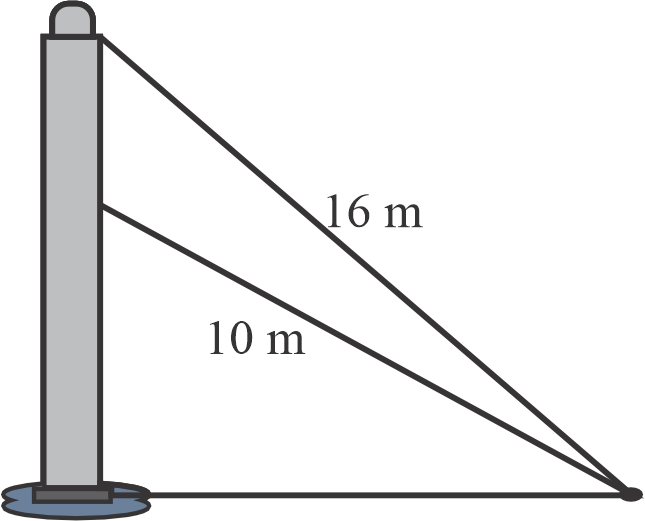
\includegraphics[width=4.5cm]{imagenes/CEPRE-UNA2024-I/etapa1/ing/geo2c24-I.png}
\end{center}


\begin{enumerate}[label=\alph*)]
	\item $25^\circ$
	\item $23^\circ$
	\item $20^\circ$
	\item $28^\circ$
	\item $18^\circ$
\end{enumerate}

\textbf{Respuesta correcta:} b)

\vspace{2mm}
\textbf{Solucionario:}\\

	\begin{center}
	\begin{minipage}{0.45\textwidth}
		En $\triangle BDC$ es notable $(30^\circ;60^\circ)$\\
		$\Rightarrow AC = 8\,m$\\
		Según los lados el $\triangle DAC$; es notable $(37^\circ,53^\circ)$\\
		Luego del $\triangle BDC$: $53^\circ = x + 30^\circ \Rightarrow x = 53^\circ - 30^\circ$\\
		$x = 23^\circ$

		
		\vspace{6mm}
	\end{minipage}
	\hfill
	\begin{minipage}{0.45\textwidth}
		\centering
		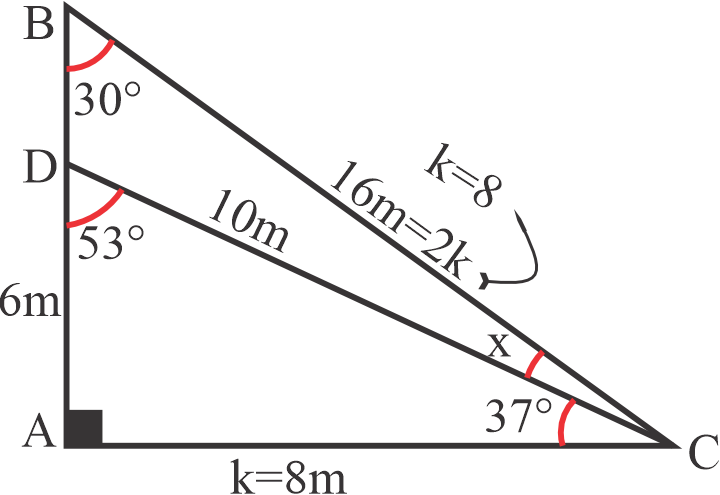
\includegraphics[width=5.5cm]{imagenes/CEPRE-UNA2024-I/etapa1/ing/geo2c24-Ir.png}
	\end{minipage}
\end{center}
\vspace{6mm}


\item Una hoja de papel rectangular de $8\pi\,m$ y $4\,m$, se dobla de tal manera que se obtiene un cilindro de altura igual a la dimensión menor del rectángulo. Halle el volumen del sólido.

\begin{enumerate}[label=\alph*)]
	\item $36\pi\,m^{3}$
	\item $48\pi\,m^{3}$
	\item $64\pi\,m^{3}$
	\item $54\pi\,m^{3}$
	\item $50\pi\,m^{3}$
\end{enumerate}

\textbf{Respuesta correcta:} c)

\vspace{2mm}
\textbf{Solucionario:}\\

\begin{center}
\begin{minipage}{0.45\textwidth}
		Pide: volumen del cilindro\\
		Se sabe que \quad $L = 2\pi R$\\
		$8\pi = 2\pi R \Rightarrow R = 4$\\
		Entonces:\quad $V = \pi r^{2}h = \pi(4)^{2}(4)$\\
		$V = 64\pi\,m^{3}$
		
		
		\vspace{6mm}
	\end{minipage}
	\hfill
	\begin{minipage}{0.45\textwidth}
		\centering
		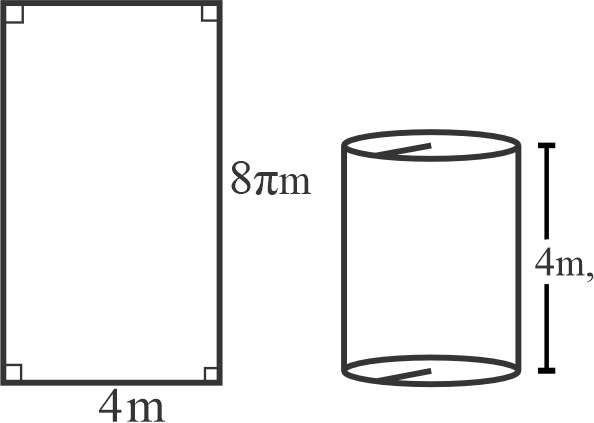
\includegraphics[width=4.5cm]{imagenes/CEPRE-UNA2024-I/etapa1/ing/geo3c24-I.png}
	\end{minipage}
\end{center}
\vspace{6mm}




\item Sobre una recta se toman los puntos consecutivos $A,\ B,\ C,\ D,\ E$ y $F$, tal que
$AC + BD + CE + DF = 26\,m$ y $BE=\left(\dfrac{5}{8}\right)AF$.\\
Calcule $AF$.

\begin{enumerate}[label=\alph*)]
	\item $12\,m$
	\item $13\,m$
	\item $16\,m$
	\item $18\,m$
	\item $20\,m$
\end{enumerate}

\textbf{Respuesta correcta:} c)

\vspace{2mm}
\textbf{Solucionario:}\\

$AF = ?$\\
Dato:\quad $BE=\dfrac{5}{8}AF$\\
Del dato:\quad $AC+BD+CE+DF=26$\\
Agrupando en forma conveniente:\quad $AE+BF=26$\\
Luego, desdoblamos $BF$:\quad $AE+(BE+EF)=26$\\
$\Rightarrow AF+BE=26$\\
Con el dato:\quad $AF+\dfrac{5}{8}AF=26$\\
Esto es:\quad $\dfrac{13}{8}AF=26$\\
$AF=16$

\end{enumerate}






\subsection*{Trigonometría}


\begin{enumerate}
	
	\item Calcule el dominio de la función real $f:$\\
	$f(x)=\dfrac{2}{\operatorname{sen}x.\cos x}$
	
	\begin{enumerate}[label=\alph*)]
		\item $\mathbb{R}-\left\{\dfrac{n\pi}{5},\, n\in\mathbb{Z}\right\}$
		\item $\mathbb{R}-\left\{\dfrac{n\pi}{3},\, n\in\mathbb{Z}\right\}$
		\item $\mathbb{R}-\left\{\dfrac{n\pi}{4},\, n\in\mathbb{Z}\right\}$
		\item $\mathbb{R}-\left\{n\pi,\, n\in\mathbb{Z}\right\}$
		\item $\mathbb{R}-\left\{\dfrac{n\pi}{2},\, n\in\mathbb{Z}\right\}$
	\end{enumerate}
	
	\textbf{Respuesta correcta:} e)
	
	\vspace{2mm}
	\textbf{Solucionario:}\\
	$f(x)=\dfrac{2\cdot 2}{2\cdot \operatorname{Sen}x\,\operatorname{Cos}x}
	=\dfrac{4}{\operatorname{Sen}(2x)}$\\
	$\operatorname{Dom}(f)=\left\{x\in\mathbb{R}\ /\ \operatorname{Sen}(2x)\neq 0\right\}$\\
	$2x\neq 0,\ \pi,\ 2\pi,\ 3\pi,\ \cdots$\\
	$2x\neq n\pi,\quad n\in\mathbb{Z}$\\
	$x\neq \dfrac{n\pi}{2},\quad n\in\mathbb{Z}$\\
	$\boxed{\operatorname{Dom}(f)=\mathbb{R}-\left\{\dfrac{n\pi}{2},\ n\in\mathbb{Z}\right\}}$
	
	
	\item En el gráfico, calcule $x$
	
	% (Dejar aquí el gráfico)
		\begin{center}
			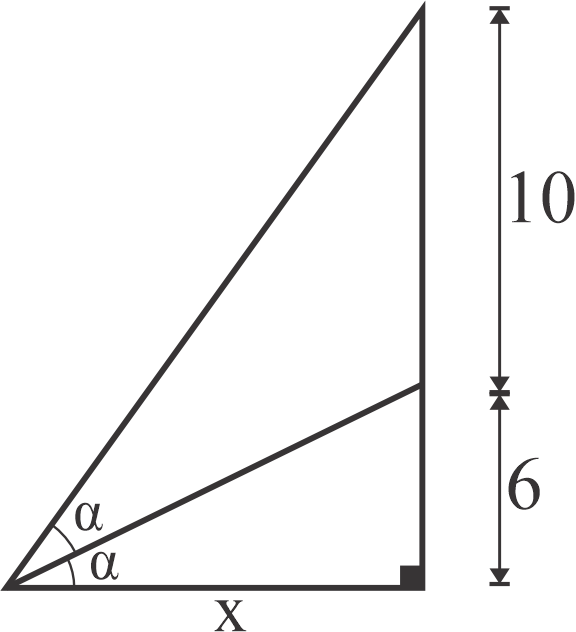
\includegraphics[width=4.5cm]{imagenes/CEPRE-UNA2024-I/etapa1/ing/trigonometria2c24-I.png}
		\end{center}

	
	\begin{enumerate}[label=\alph*)]
		\item $9$
		\item $10$
		\item $14$
		\item $12$
		\item $18$
	\end{enumerate}
	
	\textbf{Respuesta correcta:} d)
	
	\vspace{2mm}
	\textbf{Solucionario:}\\
	\begin{center}
	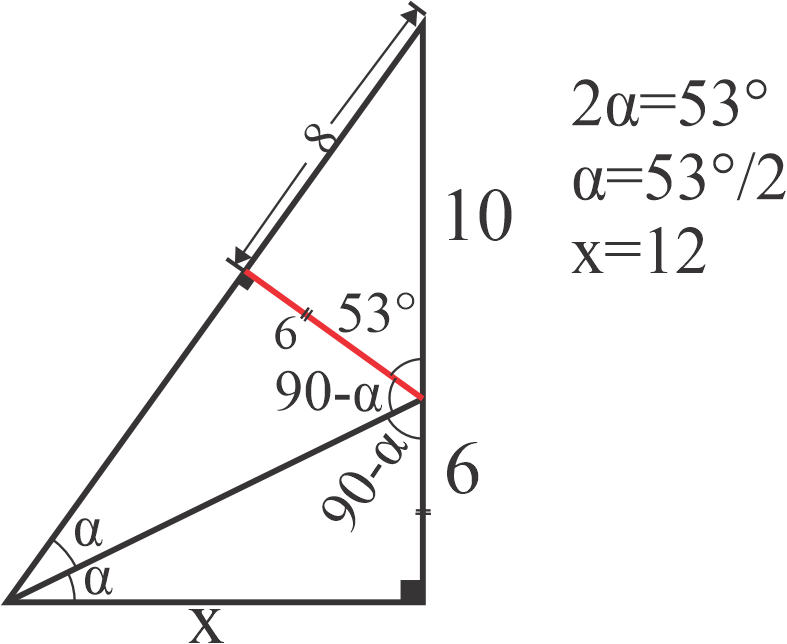
\includegraphics[width=5.5cm]{imagenes/CEPRE-UNA2024-I/etapa1/ing/trigonometria2c24-Ir.png}
	\end{center}
	
	
	\item Dos personas parten de un mismo punto. El primero recorre $3\,m$ al este y $7\,m$ al norte. El segundo recorre $5\,m$ al oeste y $8\,m$ al sur. Calcule la distancia entre las personas.
	
	\begin{enumerate}[label=\alph*)]
		\item $12\,m$
		\item $15\,m$
		\item $16\,m$
		\item $17\,m$
		\item $25\,m$
	\end{enumerate}
	
	\textbf{Respuesta correcta:} d)
	
	\vspace{2mm}
	\textbf{Solucionario:}\\

	
	
	
	
		\begin{center}
		\begin{minipage}{0.45\textwidth}
			$d(A,B)=\sqrt{(3-(-5))^{2}+(7-(-8))^{2}}$\\
			$=\sqrt{(3+5)^{2}+(7+8)^{2}}$\\
			$=\sqrt{8^{2}+15^{2}}$\\
			$=\sqrt{64+225}$\\
			$=\sqrt{289}$\\
			$d(A,B)=17\,m$
				
			\vspace{6mm}
		\end{minipage}
		\hfill
		\begin{minipage}{0.45\textwidth}
			\centering
			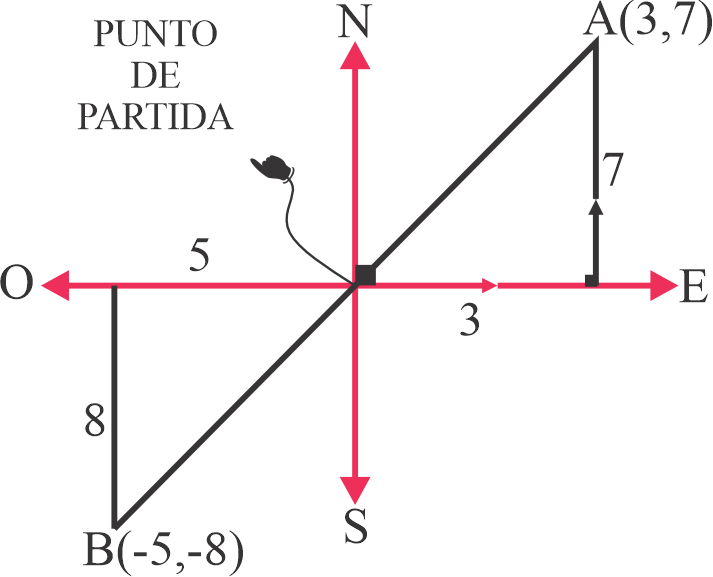
\includegraphics[width=5.5cm]{imagenes/CEPRE-UNA2024-I/etapa1/ing/trigonometria3c24-Ir.png}
		\end{minipage}
	\end{center}
	\vspace{6mm}
	
	\item El arco de un puente es semielíptico con eje mayor horizontal. Si la base mide $20\,m$ y su parte más alta con respecto al suelo es $6\,m$, determine la altura del arco trazado desde el foco de la elipse.
	
	\begin{enumerate}[label=\alph*)]
		\item $2,4\,m$
		\item $6,4\,m$
		\item $3,6\,m$
		\item $6\,m$
		\item $4\,m$
	\end{enumerate}
	
	\textbf{Respuesta correcta:} c)
	
	\vspace{2mm}
	\textbf{Solucionario:}\\
	
	\begin{center}
	\begin{minipage}{0.45\textwidth}
			$E=\dfrac{x^{2}}{10^{2}}+\dfrac{y^{2}}{36}=1$\\
		$a^{2}=b^{2}+c^{2}$\\
		$10^{2}=6^{2}+c^{2}\Rightarrow$\\
		$100=36+c^{2}$\\
		$64=c^{2}\Rightarrow \boxed{c=8}$\\
		$F(\pm 8,0)$\\
		$P=(8,h)\in E$\\
		$\dfrac{64}{100}+\dfrac{h^{2}}{36}=1$\\
		$\dfrac{h^{2}}{36}=1-\dfrac{64}{100}$\\
		$\dfrac{h^{2}}{36}=\dfrac{100-64}{100}$\\
		$h^{2}=\dfrac{36(36)}{100}$\\
		$h=\dfrac{36}{10}\Rightarrow \boxed{h=3,6\,m}$\\
		$h=\dfrac{b^{2}}{a}=\dfrac{36}{10}=3,6$
			
			\vspace{6mm}
	\end{minipage}
		\hfill
		\begin{minipage}{0.45\textwidth}
			\centering
			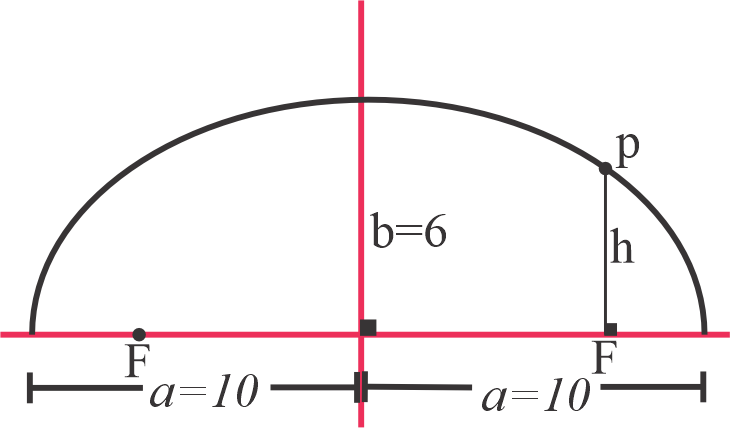
\includegraphics[width=5.5cm]{imagenes/CEPRE-UNA2024-I/etapa1/ing/trigonometria4c24-Ir.png}
		\end{minipage}
	\end{center}
	\vspace{6mm}
	
	
\end{enumerate}


\subsection*{Física}

\begin{enumerate}
	
\item Si el tablón homogéneo en la figura tiene una masa de $20\,kg$ y $4\,m$ de longitud permanece en posición horizontal, determine el valor de $x$. $(g=10\,m/s^{2})$

% (Dejar aquí el gráfico)
\begin{center}
	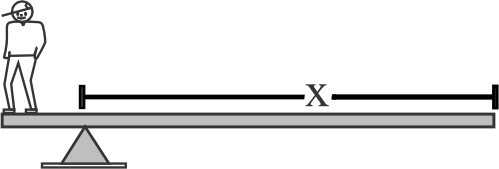
\includegraphics[width=5.5cm]{imagenes/CEPRE-UNA2024-I/etapa1/ing/Fisica1c2024-I.png}
\end{center}

\begin{enumerate}[label=\alph*)]
	\item $2,0\,m$
	\item $3,0\,m$
	\item $3,5\,m$
	\item $3,6\,m$
	\item $2,4\,m$
\end{enumerate}

\textbf{Respuesta correcta:} c)

\vspace{2mm}
\textbf{Solucionario:}\\
	\begin{center}
	\begin{minipage}{0.45\textwidth}
		2do Condición de equilibrio\\
		$\sum M=0$\\
		$600(4-x)=200(x-2)$\\
		$2400-600x=200x-400$\\
		$2800=800x$\\
		$3,5m=x$

		\vspace{6mm}
	\end{minipage}
	\hfill
	\begin{minipage}{0.45\textwidth}
		\centering
		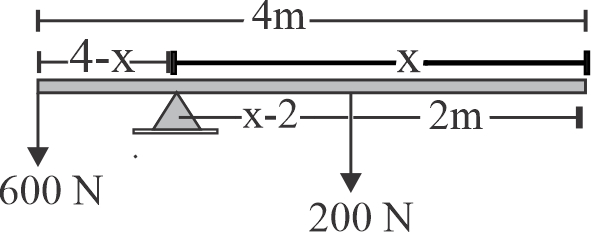
\includegraphics[width=5.5cm]{imagenes/CEPRE-UNA2024-I/etapa1/ing/Fisica1c2024-Ir.png}
	\end{minipage}
\end{center}
\vspace{6mm}



\item Una esfera de masa $m=10\,kg$ está atada a una cuerda sin peso y se mueve con MCU en una circunferencia de radio $R=2\,m$. Un bloque de masa $M=200\,kg$ se encuentra atado al otro extremo de la cuerda y pasa por un agujero en el centro de la circunferencia. Halle la rapidez angular $\omega$ de la esfera. $(g=10\,m/s^{2})$

% (Dejar aquí el gráfico)
\begin{center}
	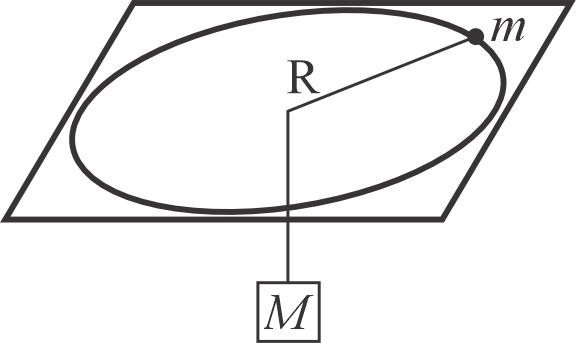
\includegraphics[width=5.5cm]{imagenes/CEPRE-UNA2024-I/etapa1/ing/Fisica2c2024-I.png}
\end{center}

\begin{enumerate}[label=\alph*)]
	\item $20\,rad/s$
	\item $30\,rad/s$
	\item $10\,rad/s$
	\item $40\,rad/s$
	\item $15\,rad/s$
\end{enumerate}

\textbf{Respuesta correcta:} c)

\vspace{2mm}
\textbf{Solucionario:}\\
Solución\\
$T=P_{B}$\\
$m\omega^{2}R=Mg$\\
$\omega=\sqrt{\dfrac{Mg}{mR}}$\\
$\omega=\sqrt{\dfrac{200(10)}{10(2)}}\ rad/s$\\
$\omega=\sqrt{100}\ rad/s$\\
$\omega=10\ rad/s$


\item Un tronco de madera de $8\,m^{3}$ de volumen flota en agua salada de densidad $1200\,kg/m^{3}$. Si el volumen emergente es de $2\,m^{3}$, determine la densidad de la madera.

	\begin{center}
	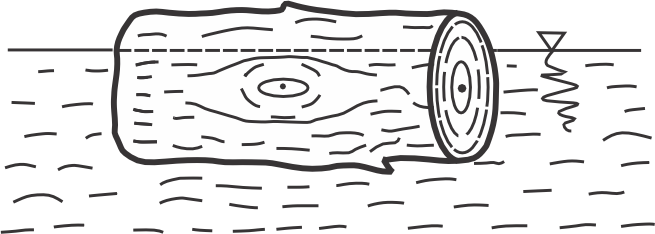
\includegraphics[width=6.5cm]{imagenes/CEPRE-UNA2024-I/etapa1/ing/Fisica3c2024-I.png}
	\end{center}

\begin{enumerate}[label=\alph*)]
	\item $300\,kg/m^{3}$
	\item $600\,kg/m^{3}$
	\item $900\,kg/m^{3}$
	\item $800\,kg/m^{3}$
	\item $700\,kg/m^{3}$
\end{enumerate}

\textbf{Respuesta correcta:} c)

\vspace{2mm}
\textbf{Solucionario:}\\





	\begin{center}
	\begin{minipage}{0.45\textwidth}

		$E=P$\\
		$m_{\ell}g=m_{m}g$\\
		$\rho_{\ell}V_{\ell}g=\rho_{m}V_{m}g$\\
		$1200(8)=\rho_{m}(8)$\\
		$1200(6)=\rho_{m}(8)$\\
		$900\,kg/m^{3}=\rho_{madera}$
		
		\vspace{6mm}
	\end{minipage}
	\hfill
	\begin{minipage}{0.45\textwidth}
		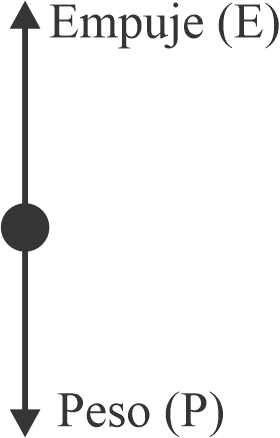
\includegraphics[width=2.4 cm]{imagenes/CEPRE-UNA2024-I/etapa1/ing/Fisica3c2024-Ir.png}
	\end{minipage}
\end{center}
\vspace{6mm}




\item En la figura, halle el ángulo $\theta$ $(n_{vidrio}=3/2\ y\ n_{agua}=4/3)$
	
\begin{center}
	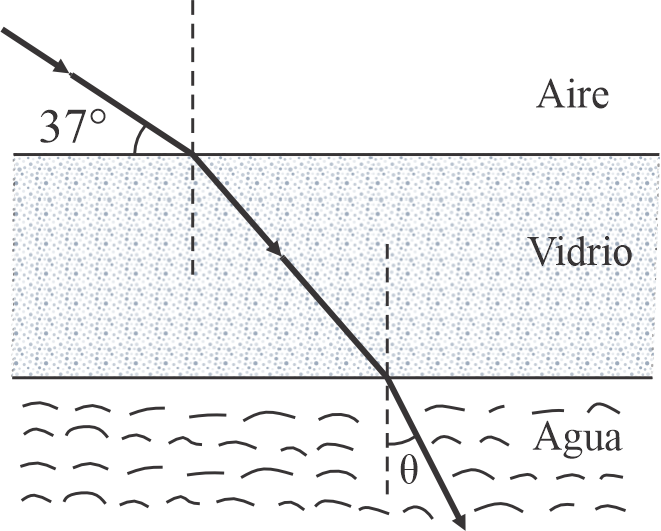
\includegraphics[width=6.5cm]{imagenes/CEPRE-UNA2024-I/etapa1/ing/Fisica4c2024-I.png}
\end{center}

\begin{enumerate}[label=\alph*)]
	\item $30^\circ$
	\item $37^\circ$
	\item $45^\circ$
	\item $53^\circ$
	\item $60^\circ$
\end{enumerate}

\textbf{Respuesta correcta:} b)

\vspace{2mm}
\textbf{Solucionario:}\\
Solución\\
(1) Aire - Vidrio\\
$n_{1}\operatorname{sen}\theta_{1}=n_{2}\operatorname{sen}\theta_{2}$\\
$\dfrac{4}{5}\times\dfrac{2}{3}=\operatorname{sen}\theta_{2}$\\
(2) Vidrio - Agua\\
$n_{2}\operatorname{sen}\theta_{2}=n_{3}\operatorname{sen}\theta_{3}$\\
$\dfrac{3}{2}\times\dfrac{4}{5}\times\dfrac{2}{3}=\dfrac{4}{3}\operatorname{sen}\theta_{3}$\\
$\dfrac{4}{5}\times\dfrac{3}{4}=\operatorname{sen}\theta_{3}$\\
$\dfrac{3}{5}=\operatorname{sen}\theta_{3}$\\
$\theta_{3}=\theta$\\
$37^\circ=\theta$
	
	
\end{enumerate}



\subsection*{Química}

\begin{enumerate}

\item Cuando la materia (electrón) choca con la antimateria (positrón), se efectúa una reacción de fusión nuclear sin dejar masa residual. Determine la energía desprendida al chocar un electrón $(e^-)$ con un positrón $(p)$ \\
$(m_{e^-}=m_{p}=9,1\times10^{-28}\,g)$

\begin{enumerate}[label=\alph*)]
	\item $164\times10^{18}\,Erg$
	\item $16,38\times10^{-20}\,Erg$
	\item $164\times10^{10}\,J$
	\item $163,8\times10^{-15}\,J$
	\item $1,638\times10^{13}\,Erg$
\end{enumerate}

\textbf{Respuesta correcta:} d)

\vspace{2mm}
\textbf{Solucionario:}\\
$E=m_{total}\,c^{2}$ $\Longrightarrow$ $m_{total}=m_{e}+m_{p}=2$\\
$E=2(9,1\times10^{-28}\,g)\,(3\times10^{10}\,cm/s)^{2}$\\
$E=(18,2\times10^{-28}\,g)\,(9\times10^{20}\,cm^{2}/s^{2})$\\
$E=163,8\times10^{-8}\,erg \times \dfrac{1J}{10^{7}\,erg}$\\
$E=163,8\times10^{-8}\times10^{-7}\,J$\\
$E=163,8\times10^{-15}\,J$


\item Al balancear la ecuación: \\
$H_{2}SO_{4}+Fe(OH)_{3}\rightarrow Fe_{2}(SO_{4})_{3}+H_{2}O$\\
La suma de los coeficientes de los productos es:

\begin{enumerate}[label=\alph*)]
	\item $3$
	\item $5$
	\item $6$
	\item $7$
	\item $4$
\end{enumerate}

\textbf{Respuesta correcta:} d)

\vspace{2mm}
\textbf{Solucionario:}\\

$3H_{2}SO_{4}+2Fe(OH)_{3}\rightarrow Fe_{2}(SO_{4})_{3}+6H_{2}O$\\
$1Fe_{2}(SO_{4})_{3}+6H_{2}O$\\
$1+6$\\
$7$


\item La ecuación de gases ideales se cumple estrictamente para casos ideales. Sin embargo, el comportamiento de los gases reales difiere del ideal a causa del tamaño de las moléculas y también porque existen fuerzas intermoleculares. No obstante, para calcular los gases reales estos se comportan como ideales especialmente a bajas presiones y elevadas temperaturas. ¿Cuántos gramos de gas Oxígeno hay en un recipiente de $82$ litros a $0,3$ atm y $27^\circ C$?

\begin{enumerate}[label=\alph*)]
	\item $24\,g$
	\item $8\,g$
	\item $64\,g$
	\item $16\,g$
	\item $32\,g$
\end{enumerate}

\textbf{Respuesta correcta:} e)

\vspace{2mm}
\textbf{Solucionario:}\\
\quad $m=?$ \quad $P=0,3\,atm$ \quad $V=82\,L$ \quad $T^\circ=27^\circ C=300^\circ K$\\
$PV=uRT$ \hfill $n=\dfrac{w}{Pm}$\\
$PV=\dfrac{w}{Pm}RT$ \hfill $w=\dfrac{PV\,Pm}{RT}$\\
$Pm_{O_{2}}=32\,g/mol$\\
$w=\dfrac{(0,3\,atm)(82\,L)(32\,g/mol)}{(0,082\,\frac{atm\cdot L}{mol\cdot {}^\circ K})(300^\circ K)}=32\,g$


\item Indique el nombre del compuesto:

\begin{center}
	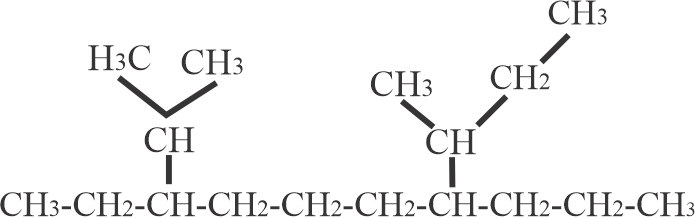
\includegraphics[width=8.4 cm]{imagenes/CEPRE-UNA2024-I/etapa1/ing/quimica4c24-I.png}
\end{center}

\begin{enumerate}[label=\alph*)]
	\item $3$-isopropil-$7$-isobutil nonano
	\item $7$-secbutil-$3$-isopropil undecano
	\item $3$-etil-$2,8$-dimetil-$7$-propil decano
	\item $8$-etil-$3,9$-dimetil-$4$-propildecano
	\item $3$-etil-$7$-butildecano
\end{enumerate}

\textbf{Respuesta correcta:} c)

\vspace{2mm}
\textbf{Solucionario:}\\
\begin{center}
	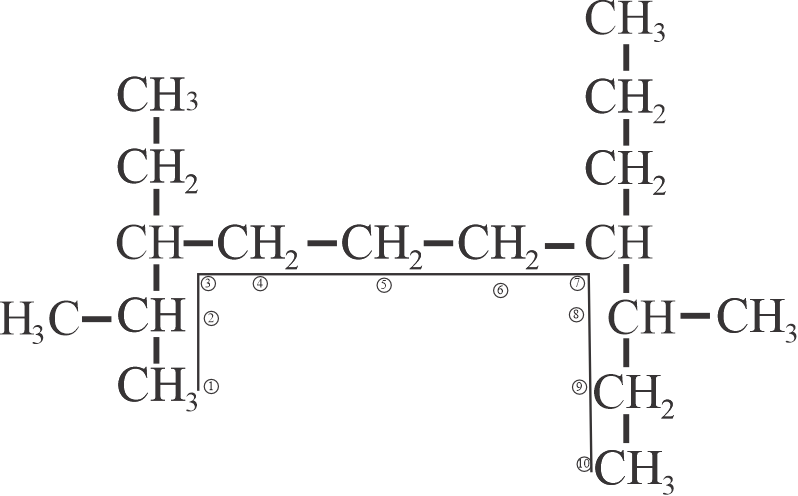
\includegraphics[width=6.4 cm]{imagenes/CEPRE-UNA2024-I/etapa1/ing/quimica4c24-Ir.png}
\end{center}

$3$-etil- $2,8$-dimetil-$7$-propil - decano\\
$3$-etil-$2,8$-dimetil-$7$-propil decano



\end{enumerate}



\subsection*{Biología y Anatomía}

\begin{enumerate}
	
	\item  ¿Qué riesgo podría pasar si un paciente presenta deficiencia de linfocitos N K?
	\begin{enumerate}[label=\alph*)]
		\item Desarrollar tumores
		\item Tuberculosis
		\item Tétanos
		\item Enfermedad de Cushing
		\item Hipotiroidismo
	\end{enumerate}
	
	\textbf{Respuesta correcta:} a)
	
	\vspace{2mm}
	\textbf{Solucionario:}\\
	Los linfocitos \textbf{NK} destruyen células tumorales y células infectadas por virus; su déficit aumenta riesgo de \textbf{tumores}.
	
	\item  ¿Cuál de las células realiza meiosis?
	\begin{enumerate}[label=\alph*)]
		\item Espermatogonía
		\item Espermatozoides
		\item Miocito y ovogonia
		\item Espermatocito primario
		\item Ovocito y ovotide
	\end{enumerate}
	
	\textbf{Respuesta correcta:} d)
	
	\vspace{2mm}
	\textbf{Solucionario:}\\
	La \textbf{meiosis} ocurre en células germinales en división; en el varón la inicia el \textbf{espermatocito primario}.
	
\end{enumerate}


\subsection*{Psicología y Filosofía}

\begin{enumerate}
	
	\item  En todo acto de conocer, se distinguen tres elementos esenciales que no pueden faltar:
	\begin{enumerate}[label=\alph*)]
		\item objeto -- idea -- memoria.
		\item sujeto -- objeto -- idea.
		\item sujeto -- inteligencia -- precepto.
		\item sujeto -- imagen -- idea.
		\item necesidad -- contingencia -- universalidad.
	\end{enumerate}
	
	\textbf{Respuesta correcta:} b)
	
	\vspace{2mm}
	\textbf{Solucionario:}\\
	En el acto de conocer intervienen \textbf{sujeto} (quien conoce), \textbf{objeto} (lo conocido) e \textbf{idea/representación}.
	
	\item  Según Jean Piaget, la asimilación y acomodación son elementos determinantes de:
	\begin{enumerate}[label=\alph*)]
		\item conciencia.
		\item desarrollo de esquemas motores.
		\item nivel intelectual del individuo.
		\item adaptación.
		\item codificación de la conducta.
	\end{enumerate}
	
	\textbf{Respuesta correcta:} d)
	
	\vspace{2mm}
	\textbf{Solucionario:}\\
	Para Piaget, asimilación y acomodación forman parte del proceso de \textbf{adaptación} cognitiva.
	
	\item  Es el proceso por el cual el individuo adquiere conocimientos, destrezas y nuevos modos de comportamiento que le permiten alcanzar con mayor eficacia sus objetivos y satisfacer sus necesidades.
	\begin{enumerate}[label=\alph*)]
		\item La adaptación.
		\item La sensación.
		\item La atención.
		\item La memoria.
		\item El aprendizaje.
	\end{enumerate}
	
	\textbf{Respuesta correcta:} e)
	
	\vspace{2mm}
	\textbf{Solucionario:}\\
	La definición corresponde a \textbf{aprendizaje}: cambio relativamente estable por experiencia.
	
	\item  Cuando una persona tiene miedo y preocupación de padecer o tener una enfermedad grave a partir de la interpretación subjetiva que hace de uno o más síntomas o signos, se infiere que presenta un trastorno:
	\begin{enumerate}[label=\alph*)]
		\item depresivo.
		\item hipocondríaco.
		\item fóbico.
		\item obsesivo compulsivo.
		\item de ansiedad.
	\end{enumerate}
	
	\textbf{Respuesta correcta:} b)
	
	\vspace{2mm}
	\textbf{Solucionario:}\\
	La preocupación persistente por tener una enfermedad grave por interpretar síntomas se asocia a la \textbf{hipocondría} (ansiedad por la enfermedad).
	
	
\end{enumerate}






\subsection*{Geografía}

\begin{enumerate}


\item Son áreas nacionales destinadas a la protección y preservación con carácter intangible, de asociaciones naturales de fauna y flora silvestre.
\begin{enumerate}[label=\alph*)]
	\item Zonas de reserva
	\item Santuarios históricos
	\item Santuarios nacionales
	\item Reservas nacionales
	\item Parques nacionales
\end{enumerate}

\textbf{Respuesta correcta:} e)

\vspace{2mm}
\textbf{Solucionario:}\\
Los \textbf{parques nacionales} son áreas naturales protegidas \textbf{intangibles}, destinadas a la protección y preservación de asociaciones naturales de fauna y flora silvestre.

\item  Es el número de nacimientos ocurridos en un año por cada 1,000 habitantes. La expresión se representa porcentualmente.
\begin{enumerate}[label=\alph*)]
	\item Tasa bruta de natalidad
	\item Tasa bruta de fecundidad
	\item Tasa bruta de reproducción
	\item Tasa bruta de crecimiento poblacional
	\item Esperanza de vida al nacer
\end{enumerate}

\textbf{Respuesta correcta:} a)

\vspace{2mm}
\textbf{Solucionario:}\\
La definición corresponde a la \textbf{tasa bruta de natalidad}: nacimientos por cada 1000 habitantes en un año.




\end{enumerate}







\subsection*{Historia}

\begin{enumerate}

\item  Explotación con rasgos feudales realizado a los campesinos ubicados dentro o fuera de las haciendas, especialmente en la sierra sur.
\begin{enumerate}[label=\alph*)]
	\item Cooperativismo
	\item Gamonalismo
	\item Civilismo
	\item Socialismo
	\item Imperialismo
\end{enumerate}

\textbf{Respuesta correcta:} b)

\vspace{2mm}
\textbf{Solucionario:}\\
El \textbf{gamonalismo} fue una forma de dominación y explotación de campesinos ligada al poder de los hacendados.

\item  La cultura Paracas pertenece al periodo ................................ mientras que cultura Wari perteneció al periodo ....................................
\begin{enumerate}[label=\alph*)]
	\item Horizonte temprano -- Horizonte medio
	\item Horizonte medio -- Intermedio tardio
	\item Arcaico temprano -- Intermedio tardio
	\item Arcaico tardio -- Formativo inicial
	\item Formativo final -- Pre cerámico
\end{enumerate}

\textbf{Respuesta correcta:} a)

\vspace{2mm}
\textbf{Solucionario:}\\
Paracas se ubica en el \textbf{Horizonte temprano} (transición formativa), y Wari corresponde al \textbf{Horizonte medio}.

\end{enumerate}


\subsection*{Educación Cívica}

\begin{enumerate}


\item  Es aquel documento que toda persona jurídica debe tener mediante escritura pública, en el cual debe constar su denominación, domicilio, objetivos, actividades, deberes y derechos de sus integrantes.
\begin{enumerate}[label=\alph*)]
	\item Estatuto
	\item Reglamento
	\item Acta de socios
	\item Acta de conformación de la junta directiva
	\item Libros de Actas
\end{enumerate}

\textbf{Respuesta correcta:} a)

\vspace{2mm}
\textbf{Solucionario:}\\
El documento base que regula la organización y funcionamiento de una persona jurídica es el \textbf{estatuto}.

\item  A consecuencia de un accidente de tránsito, el Presidente de la República y sus dos vicepresidentes sufrieron lesiones de consideración. Posteriormente, fueron evacuados a la ciudad de Piura donde fueron hospitalizados. Según las normas constitucionales, en un caso como este, la Presidencia de la República es asumida por el presidente:
\begin{enumerate}[label=\alph*)]
	\item de la Corte Suprema.
	\item del Congreso de la República.
	\item del Tribunal Constitucional.
	\item del Consejo de Ministros.
	\item del Consejo Nacional de la Magistratura.
\end{enumerate}

\textbf{Respuesta correcta:} b)

\vspace{2mm}
\textbf{Solucionario:}\\
Si no pueden asumir el Presidente ni los vicepresidentes, la sucesión recae en el \textbf{Presidente del Congreso}.

\end{enumerate}






\subsection*{Economía}

\begin{enumerate}


\item ¿Cuál de los productos está gravado con el Impuesto Selectivo al Consumo (ISC) en el Perú?
\begin{enumerate}[label=\alph*)]
	\item Agua potable
	\item Gasolina
	\item Harina de trigo
	\item Papel
	\item Arroz pilado
\end{enumerate}

\textbf{Respuesta correcta:} b)

\vspace{2mm}
\textbf{Solucionario:}\\
El ISC grava bienes específicos (p.ej. combustibles). La \textbf{gasolina} está afecta al ISC.

\item  Es el proceso de traslado e intercambio de mercancías (bienes, servicios y factores de producción) que permite la integración de la producción y el consumo.
\begin{enumerate}[label=\alph*)]
	\item Producción
	\item Circulación
	\item Distribución
	\item Consumo
	\item Exportación
\end{enumerate}

\textbf{Respuesta correcta:} b)

\vspace{2mm}
\textbf{Solucionario:}\\
El traslado e intercambio que conecta producción con consumo corresponde a la \textbf{circulación}.


\end{enumerate}


\subsection*{Comunicación}

\begin{enumerate}



\item  Más vale pájaro en mano ...\\
Los puntos suspensivos de la frase indican que:
\begin{enumerate}[label=\alph*)]
	\item anuncia una serie de palabras.
	\item se interrumpe una enumeración.
	\item reitera un término.
	\item el texto está incompleto.
	\item el texto está completo.
\end{enumerate}

\textbf{Respuesta correcta:} d)

\vspace{2mm}
\textbf{Solucionario:}\\
Los puntos suspensivos indican \textbf{omisión} de una parte del enunciado (queda incompleto).

\item Carlos abre las páginas de un periódico. Lee una columna periodística y toma conciencia de que está leyendo.
\begin{enumerate}[label=\alph*)]
	\item una sumilla.
	\item un texto.
	\item un párrafo.
	\item un resumen.
	\item una conclusión.
\end{enumerate}

\textbf{Respuesta correcta:} b)

\vspace{2mm}
\textbf{Solucionario:}\\
Una columna periodística es un \textbf{texto} (unidad comunicativa completa).

\item  Los átomos raramente se encuentran libres.\\
Tienden a agruparse formando moléculas.\\
El enunciado utiliza el lenguaje:
\begin{enumerate}[label=\alph*)]
	\item coloquial o familiar.
	\item protocolar o estándar.
	\item técnico o especializado.
	\item visual o pictórico.
	\item jerga o parasitaria.
\end{enumerate}

\textbf{Respuesta correcta:} c)

\vspace{2mm}
\textbf{Solucionario:}\\
Usa terminología científica (\textbf{átomos}, \textbf{moléculas}), por eso es \textbf{técnico}.

\item  Un alumno del CEPREUNA duda entre decir ``tú'' y ``usted'' para dirigirse a su docente de Lengua. En este acto, el alumno busca la:
\begin{enumerate}[label=\alph*)]
	\item cohesión del discurso.
	\item adecuación del discurso.
	\item información correspondiente.
	\item identificación del discurso.
	\item expresión de un punto de vista.
\end{enumerate}

\textbf{Respuesta correcta:} b)

\vspace{2mm}
\textbf{Solucionario:}\\
Elegir entre ``tú''/``usted'' es ajustar el registro al contexto: \textbf{adecuación}.

\end{enumerate}



\subsection*{Literatura}

\begin{enumerate}

\item  La obra de Garcilaso de la Vega, ``Comentarios reales de los Incas'', se clasifica como una:
\begin{enumerate}[label=\alph*)]
	\item novela.
	\item cuento.
	\item crónica.
	\item epístola.
	\item égloga.
\end{enumerate}

\textbf{Respuesta correcta:} c)

\vspace{2mm}
\textbf{Solucionario:}\\
Es una obra historiográfica/testimonial, por ello se considera una \textbf{crónica}.

\item  En la ``Divina Comedia'', en el noveno círculo del Infierno, Dante se encuentra con Lucifer; quién posee tres cabezas: una roja, una amarilla y una negra, las cuales simbolizan respectivamente:
\begin{enumerate}[label=\alph*)]
	\item odio, impotencia e ignorancia.
	\item avaricia, lujuria y soberbia.
	\item impotencia, hambre y odio.
	\item ignorancia, avaricia y soberbia.
	\item pasión, debilidad y maldad.
\end{enumerate}

\textbf{Respuesta correcta:} a)

\vspace{2mm}
\textbf{Solucionario:}\\
Las tres cabezas se interpretan como \textbf{odio}, \textbf{impotencia} e \textbf{ignorancia}.
\end{enumerate}


\subsection*{Razonamiento Matemático}

\begin{enumerate}

\item Una persona en el mes de marzo, resta a los meses que ha vivido los años que tiene y obtiene $425$. ¿En qué mes nació?
\begin{enumerate}[label=\alph*)]
	\item Enero
	\item Mayo
	\item Junio
	\item Agosto
	\item Octubre
\end{enumerate}

\textbf{Respuesta correcta:} d)

\vspace{2mm}
\textbf{Solucionario:}\\

Supongamos que la edad de la persona es
$X$ años, y $Y$ meses.

en el mes de marzo tenemos,

(meses vividos)$=12X+Y$
(años que tiene)$=X$

$\Rightarrow\; 12X+Y-X=425$
$11X+Y=425.$

Tanto \quad $11X+Y=11(38)+7$

Luego \quad $425 \div 11 = 38$ \quad y sobra $7$.

\textbf{Actual} $\rightarrow$ \textbf{Marzo}

Como tiene $38$ años y $7$ meses

% --- TIMELINE EN HORIZONTAL (tal cual la foto) ---
\begin{tikzpicture}[x=1.2cm,y=1cm,>=Stealth]

	
	% línea principal
	\draw[thick] (-0.2,0) -- (7.2,0);
	
	% marcas + meses (arriba)
	\foreach \x/\lab in {
		0/Ago,
		1/set.,
		2/oct.,
		3/Nov.,
		4/Dic,
		5/Ene,
		6/Feb,
		7/Mar
	}{
		\draw[thick] (\x,0.28) -- (\x,-0.28);
		\node[above=6pt] at (\x,0.28) {\lab};
	}
	
	% círculo azul alrededor de "Agosto"
	\draw[blue,thick] (0,0.78) ellipse [x radius=0.59, y radius=0.28];
	
	% arcos rojos (flecha hacia la izquierda) + números en círculo
	\foreach \i/\n in {1/7,2/6,3/5,4/4,5/3,6/2,7/1}{
		% arco hacia ABAJO (debajo)
		\draw[red,thick,->] (\i,-0.35) to[bend left=55] (\i-1,-0.35);
		% número en circulito rojo debajo
		\node[red,draw,circle,inner sep=1.2pt] at (\i-0.5,-0.95) {\scriptsize \n};
	}
	
\end{tikzpicture}





\item ¿Cuál es el valor máximo que puede tener el área del rectángulo inscrito en el triángulo mostrado?

\begin{center}
	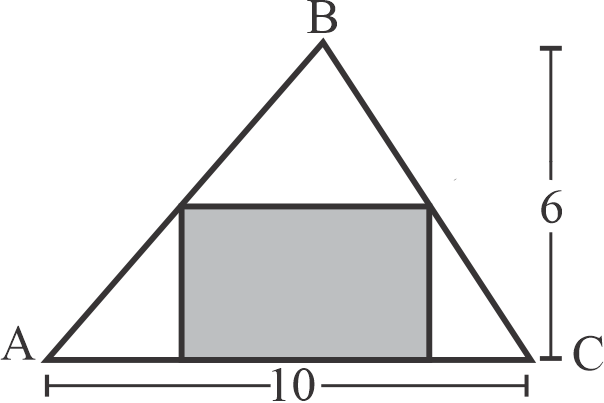
\includegraphics[width=5.5cm]{imagenes/CEPRE-UNA2024-I/etapa1/ing/rm2c24-I.png}
\end{center}


\begin{enumerate}[label=\alph*)]
	\item $15\,u^2$
	\item $20\,u^2$
	\item $30\,u^2$
	\item $45\,u^2$
	\item $40\,u^2$
\end{enumerate}

\textbf{Respuesta correcta:} a)

\vspace{2mm}
\textbf{Solucionario:}\\

	\begin{center}
	\begin{minipage}{0.45\textwidth}
$\triangle ABC \cong DBE$\\
Área dd rectángulo es:\\
\[
A = 5k(6-3k)
\]
\[
= 15k(2-k)
\]
Para q área sea máxima\\
\[
k = 2-k \Rightarrow k = 1
\]
Luego área máxima es\\
\[
A_{\max} = 15(1)(2-1) = 15
\]

		
		\vspace{6mm}
	\end{minipage}
	\hfill
	\begin{minipage}{0.45\textwidth}
		\centering
		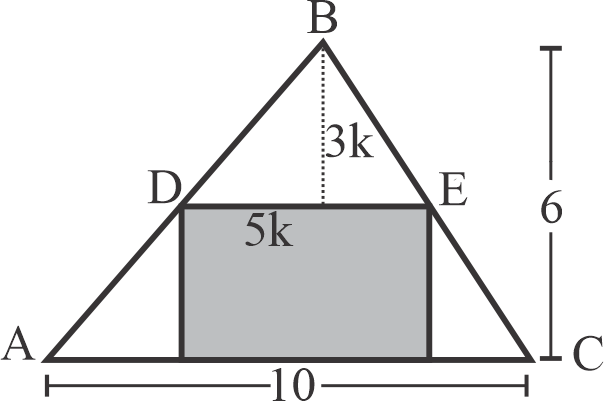
\includegraphics[width=5.5cm]{imagenes/CEPRE-UNA2024-I/etapa1/ing/rm2c24-Ir.png}
	\end{minipage}
\end{center}
\vspace{6mm}


\item Si a un número de dos cifras le restamos veintisiete, resulta el mismo número, pero con las cifras invertidas. Determine el producto de las cifras de dicho número sabiendo que la suma es nueve.
\begin{enumerate}[label=\alph*)]
	\item 18
	\item 15
	\item 17
	\item 14
	\item 12
\end{enumerate}

\textbf{Respuesta correcta:} a)

\vspace{2mm}
\textbf{Solucionario:}\\

Sea el número de dos cifras $\overline{xy}$\\
$
xy-27 = yx\\
$
$
x-y = 3\\
$
$
\Rightarrow 10x+y-27 = 10y+x\\
$
$
10x-x+y-10y = 27\\
$
$
9x-9y = 27\\
$
$
x-y = 3\\
$
luego
$
\begin{aligned}
	x+y &= 9\\
	x-y &= 3\\ \hline
	2x &= 12
\end{aligned}
$\\
donde: $x=6$, $y=3$, el numero será 63,\\
entonces el producto es: $6x3=18$





\vspace{6mm}







\item  Se define el operador:
\[
\boxed{n}=\frac{n(n+1)}{2}
\]
Además
\[
\boxed{\boxed{\boxed{2x+1}}}=21
\]
Calcule el valor de $x$.

\begin{enumerate}[label=\alph*)]
	\item 1
	\item $\dfrac{1}{2}$
	\item 2
	\item $\dfrac{3}{4}$
	\item 3
\end{enumerate}

\textbf{Respuesta correcta:} b)

\vspace{2mm}
\textbf{Solucionario:}\\

de la definición $\boxed{n}=\dfrac{n(n+1)}{2}$\\
llevemos al modelo de la regla de correspondencia\\[1mm]
$\boxed{\boxed{\boxed{2x+1}}}=21=\frac{6\times 7}{2}\ \Rightarrow\ \boxed{\boxed{2x+1}}=6$\\
$\boxed{\boxed{2x+1}}=6=\frac{3\times 4}{2}\ \Rightarrow\ \boxed{2x+1}=3$\\
$\boxed{2x+1}=3=\frac{2\times 3}{2}\ \Rightarrow\ 2x+1=2$\\
$\Rightarrow\ 2x=1$\\
$\Rightarrow\ x=\frac{1}{2}$\\
$\therefore\ \text{El valor de $x$ es }\frac{1}{2}$\\




\item La suma de 81 números pares consecutivos es igual a 171 veces el primer número. Halle la suma de cifras del término central.

\begin{enumerate}[label=\alph*)]
	\item 8
	\item 9
	\item 7
	\item 6
	\item 5
\end{enumerate}

\textbf{Respuesta correcta:} a)

\vspace{2mm}
\textbf{Solucionario:}\\[1mm]

% -]-- Tal como en la hoja ---
$\overset{1^\circ}{(x+2)}+\overset{2^\circ}{(x+4)}+\overset{3^\circ}{(x+6)}+\cdots+\overset{81^\circ}{(x+162)}=171(x+2)$\\[-7mm]

\hspace{2mm}
$\underbrace{\hspace*{75mm}}_{\text{\footnotesize 81 números pares}}$\\[-2mm]

\vspace{2mm}
\hspace*{30mm}\textbf{Suma de términos}\\[1mm]
\hspace*{1mm}$\left(\dfrac{(x+2)+(x+162)}{2}\right)\times 81 \;=\;171(x+2)$\\


$(x+82)\times 81 \;=\;171(x+2)$\\
$81x+6642 \;=\;171x+342$\\
$x=70$\\[2mm]

\textit{El término central ocupa la posición:}\\[1mm]
$\dfrac{81+1}{2}=41$\\
$\Rightarrow\ t_c=t_{41}=x+82=70+82=152$\\[2mm]

$\therefore\ \text{Suma de cifras: }1+5+2=8$





\item En una mesa circular de 7 sillas se sientan a dialogar 4 obreros: $A,B,C,D$ y 3 empleados: $X,Y,Z$. Se sabe que:
\begin{itemize}
	\item Ningún empleado se sienta junto a otro empleado.
	\item $B$ se sienta junto a $D$, pero $Z$ no se sienta junto a ellos.
\end{itemize}
Determine cuál afirmación es siempre verdadera.

\begin{enumerate}[label=\alph*)]
	\item Solo I
	\item I y II
	\item Solo II
	\item I y III
	\item Solo III
\end{enumerate}

\textbf{Respuesta correcta:} a)

\vspace{2mm}
\textbf{Solucionario:}\\[1mm]

\textbf{Obreros:} $A,B,C,D$\qquad \textbf{Empleados:} $X,Y,Z$\\[1mm]








\begin{center}
	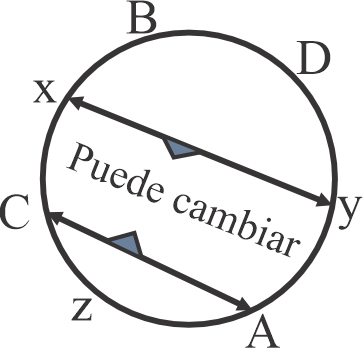
\includegraphics[width=4.5cm]{imagenes/CEPRE-UNA2024-I/etapa1/ing/rm6c24-I.png}
\end{center}






\end{enumerate}


















\subsection*{Razonamiento verbal}

\begin{enumerate}

\item Persona que camina y realiza actividades de noche se denomina:
\begin{enumerate}[label=\alph*)]
	\item sonámbulo.
	\item noctámbulo.
	\item nefando.
	\item cicatero.
	\item nocturno.
\end{enumerate}

\textbf{Respuesta correcta:} b)

\vspace{2mm}
\textbf{Solucionario:}\\
\textbf{Noctámbulo} es la persona que \textbf{acostumbra estar despierta durante la noche} y realizar actividades en ese horario (por ejemplo, trabajar o caminar de madrugada). 
En cambio, \textbf{sonámbulo} es quien camina o actúa mientras duerme (sonambulismo), \textbf{nocturno} suele usarse como adjetivo (actividad nocturna), y \textbf{nefando} / \textbf{cicatero} no se relacionan con el hábito de estar activo en la noche.

\item Complete la oración:

........... las rocas son unidades básicas de la corteza terrestre, a veces pueden aparecer al descubierto, ........... en otras ocasiones permanecen ocultas bajo el suelo, .......... generalmente, están al descubierto.

\begin{enumerate}[label=\alph*)]
	\item Si - entonces - incluso
	\item Como - mientras - aunque
	\item Siempre - puesto que - ahora
	\item Cuando - por tanto - inclusive
	\item Por que - mas - asi mismo
\end{enumerate}

\textbf{Respuesta correcta:} b)

\vspace{2mm}
\textbf{Solucionario:}\\
La opción correcta organiza la idea con conectores lógicos coherentes:
\begin{itemize}
	\item \textbf{Como} introduce una explicación o causa: “\textbf{Como} las rocas son unidades básicas...”
	\item \textbf{mientras} marca contraste de situaciones: “...a veces pueden aparecer al descubierto, \textbf{mientras} en otras ocasiones...”
	\item \textbf{aunque} añade una concesión (algo que ocurre a pesar de lo anterior): “..., \textbf{aunque} generalmente, están al descubierto.”
\end{itemize}
Así, la oración queda natural y con sentido completo, alternando explicación, contraste y concesión.

% -------------------------

\item En el gentilicio ``bonaerense'', se ha utilizado el sufijo:
\begin{enumerate}[label=\alph*)]
	\item aerense
	\item erense
	\item rense
	\item ense
	\item se
\end{enumerate}

\textbf{Respuesta correcta:} d)

\vspace{2mm}
\textbf{Solucionario:}\\
En “bonaerense” se reconoce el sufijo \textbf{-ense}, frecuente en gentilicios del español (por ejemplo: “lime\textbf{nse}”, “costarrice\textbf{nse}”). 
El sufijo es la parte final que se añade para formar la palabra y, en este caso, la terminación visible es \textbf{ense}.

% -------------------------

\item El término OCÉANO incluye:
\begin{enumerate}[label=\alph*)]
	\item montaña, valle, cañón
	\item costa, ola, marea
	\item barco, velero, submarino
	\item isla, archipiélago, embarcación
	\item Pez, delfín, ballena
\end{enumerate}

\textbf{Respuesta correcta:} b)

\vspace{2mm}
\textbf{Solucionario:}\\
La pregunta apunta a elementos que se asocian directamente con el \textbf{océano} como \textbf{cuerpo de agua} y sus fenómenos:
\textbf{costa} (límite entre mar y tierra), \textbf{ola} (movimiento del agua) y \textbf{marea} (subida y bajada periódica del nivel del mar).
Las otras alternativas contienen: relieve terrestre (A), medios de transporte (C), mezcla de accidentes geográficos y objetos (D), o fauna marina (E), que pueden existir en el océano, pero no “definen” mejor el término como fenómeno geográfico.

% -------------------------

\item Resuelva la analogía:\\
TUNGSTENO: Tg.
\begin{enumerate}[label=\alph*)]
	\item \makebox[2cm][l]{Fósforo} : \makebox[1.2cm][l]{P}
	\item \makebox[2cm][l]{Calcio}  : \makebox[1.2cm][l]{Cl}
	\item \makebox[2cm][l]{Rutenio} : \makebox[1.2cm][l]{Rt}
	\item \makebox[2cm][l]{Plata}   : \makebox[1.2cm][l]{Og}
	\item \makebox[2cm][l]{Oro}     : \makebox[1.2cm][l]{Ou}
\end{enumerate}


\textbf{Respuesta correcta:} a)

\vspace{2mm}
\textbf{Solucionario:}\\
La relación es \textbf{Elemento químico : símbolo químico}. 
Entre las opciones, la única pareja correctamente formada es \textbf{Fósforo : P}. 
Las demás tienen símbolos incorrectos (por ejemplo, el calcio es \textbf{Ca}, la plata es \textbf{Ag}, el oro es \textbf{Au}, y el rutenio es \textbf{Ru}). 
Por eso, la alternativa que mantiene la misma relación es la \textbf{a)}.

\item \textbf{COMPRENSIÓN DE TEXTO}\\
``Por eso se mueren los hombres; porque no son capaces de enlazar el principio con el fin''\\
\hfill \textit{Alcmeón de Crotona}\\[1mm]
¿Qué enunciado se adecúa mejor al texto?
\begin{enumerate}[label=\alph*)]
	\item El principio y el fin son disímiles.
	\item El hombre está confabulado en el origen y en el final.
	\item La mortalidad de los hombres implica la negación de un principio circular.
	\item La muerte de los hombres destituye el principio del fin.
	\item El fin del hombre es su muerte.
\end{enumerate}

\textbf{Respuesta correcta:} c)

\vspace{2mm}
\textbf{Solucionario:}\\
El texto afirma que los hombres mueren porque no logran \textbf{enlazar} el \textbf{principio} con el \textbf{fin}. Esa idea sugiere que comprender la vida implicaría ver una \textbf{continuidad} o \textbf{ciclo} (un “principio circular”), donde el final se conecta con el inicio. 
Si el ser humano \textbf{no puede unir} ambos extremos, entonces \textbf{no asume} o \textbf{niega} esa visión circular; y el texto asocia esa incapacidad con la \textbf{mortalidad}. 
Por ello, la opción que mejor interpreta el sentido es: \textbf{la mortalidad implica la negación de un principio circular}.


\end{enumerate}



\subsection*{Inglés}

\begin{enumerate}
	
\item Observe the picture and answer this question:\\
How is the weather in Puno?
\begin{enumerate}[label=\alph*)]
	\item It is windy.
	\item it is hot.
	\item it is raining.
	\item It is cold.
	\item It is sunny.
\end{enumerate}

\textbf{Respuesta correcta:} c)

\vspace{2mm}
\textbf{Solucionario:}\\
In the picture we can see \textbf{clouds} and \textbf{raindrops} falling down, and the person is holding an \textbf{umbrella}. Those clues clearly indicate that the weather is \textbf{rainy}. Therefore, the correct answer is: \textbf{it is raining}.

% -------------------------

\item Answer the question.\\
Which sentence has a possessive adjective?
\begin{enumerate}[label=\alph*)]
	\item They are engineers.
	\item Their names are Peter and Thomas.
	\item They are from Australia.
	\item They have modern computers.
	\item They work for ``Air France''
\end{enumerate}

\textbf{Respuesta correcta:} b)

\vspace{2mm}
\textbf{Solucionario:}\\
A possessive adjective shows \textbf{ownership} or \textbf{possession} (my, your, his, her, its, \textbf{their}, our). 
In option \textbf{b)}, the word \textbf{Their} describes the noun \textbf{names} and indicates that the names \textbf{belong to them}. The other options do not include a possessive adjective, so \textbf{b)} is correct.

\end{enumerate}



\subsection*{Quechua y Aimara}

\begin{enumerate}
	
\item ¿Mayqantaq wasi uywari? / ¿Kawkirisa uta uywaxa?
\begin{enumerate}[label=\alph*)]
	\item Taruka / Taruka
	\item Allqu / Anu
	\item Atuq / Qamaqi
	\item Añas / Añuthaya
	\item Anka / Allqamari
\end{enumerate}

\textbf{Respuesta correcta:} b)

\vspace{2mm}
\textbf{Solucionario:}\\
La pregunta apunta a identificar el \textbf{animal doméstico de casa} (wasi/uta se relaciona con “casa”). 
En quechua, \textbf{Allqu} significa \textbf{perro}; y en aimara, \textbf{Anu} también significa \textbf{perro}. 
Las demás alternativas corresponden a animales silvestres (por ejemplo, taruka, atuq) o aves (anka), por lo que no representan el “animal de casa” del modo más directo. Por eso la correcta es \textbf{Allqu / Anu}.

% -------------------------

\item ¿Hayk'a pachayuqtag huk p'unchawri kan? / ¿Qawqha pachanisa mä uruxa?
\begin{enumerate}[label=\alph*)]
	\item Iskay chunka hukniyuq / Pä tunka maya pachani
	\item Iskay chunka iskayniyuq / Pä tunka paya pachani
	\item Iskay chunka tawayuq / Pä tunka pusi pachani
	\item Iskay chunka pichqayuq / Pä tunka phisqa pachani
	\item Iskay chunka suqtayuq / Pä tunka suxta pachani
\end{enumerate}

\textbf{Respuesta correcta:} c)

\vspace{2mm}
\textbf{Solucionario:}\\
La pregunta significa: \textbf{“¿Cuántas horas tiene un día?”}. Un día tiene \textbf{24 horas}.  
En quechua, \textbf{Iskay chunka} es “20” y el segundo término agrega unidades: \textbf{tawayuq} indica “+4”, formando \textbf{24}.  
En aimara, \textbf{Pä tunka} es “20” y \textbf{pusi} es “4”, por lo que \textbf{Pä tunka pusi} también forma \textbf{24}.  
Así, la alternativa que coincide con 24 horas es \textbf{Iskay chunka tawayuq / Pä tunka pusi pachani}.

\end{enumerate}


\section*{Área: Biomédicas}





\subsection*{Aritmética}

\begin{enumerate}
	
	\item Una casa podrá ser construida por 25 albañiles en 36 días trabajando 8 horas diarias. Pero si solo trabajan 18 albañiles a razón de 10 horas diarias. ¿En cuántos días podrán construir la casa?
	\begin{enumerate}[label=\alph*)]
		\item 40
		\item 42
		\item 38
		\item 41
		\item 39
	\end{enumerate}
	\textbf{Respuesta correcta:} a)
	
	\vspace{2mm}
	\textbf{Solucionario:}\\
	
	Del problema, tenemos
	
	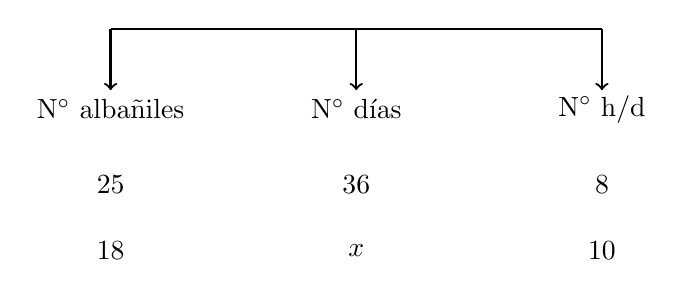
\begin{tikzpicture}[x=2.4cm,y=1.2cm]
		
		% Línea superior
		\draw[thick] (0.7,2.8) -- (3.3,2.8);
		
		% Flechas
		\draw[->, thick] (0.7,2.8) -- (0.7,2.15);
		\draw[->, thick] (2,2.8) -- (2,2.15);
		\draw[->, thick] (3.3,2.8) -- (3.3,2.15);
		
		% Encabezados
		\node at (0.7,1.95) {N$^\circ$ albañiles};
		\node at (2,1.95) {N$^\circ$ días};
		\node at (3.3,1.95) {N$^\circ$ h/d};
		
		% Primera fila
		\node at (0.7,1.15) {25};
		\node at (2,1.15) {36};
		\node at (3.3,1.15) {8};
		
		% Segunda fila
		\node at (0.7,0.45) {18};
		\node at (2,0.45) {$x$};
		\node at (3.3,0.45) {10};
		
	\end{tikzpicture}
	
	Así;
	
	$(\text{N}^\circ \text{ días})(\text{N}^\circ \text{ albañiles})(\text{N}^\circ \text{ h/d})= (36)(25)(8)=x(18)(10)$
	
	$x=40$
	
	\vspace{6mm}
	
	\item En la igualdad, halle $a$
	
	$$\overline{\underbrace{aaa\cdots}_{40\ \text{cifras}}}=\mathring{9}
	+2$$
	
	\begin{enumerate}[label=\alph*)]
		\item 8
		\item 6
		\item 4
		\item 5
		\item 9
	\end{enumerate}
	\textbf{Respuesta correcta:} d)
	
	\vspace{2mm}
	\textbf{Solucionario:}\\
	
	$\overline{aaaa\ldots}=\mathring{9}+2 \qquad \text{Criterio $\mathring{9}$}$
	
	$\underbrace{a+a+a+a+\cdots+a}_{40\ \text{cifras}}=\mathring{9}+2$
	
	$40a=\mathring{9}+2$
	
	$(\mathring{9}+4)a=\mathring{9}+2$
	
	$4a=\mathring{9}+2+18$
	
	$4a=\mathring{9}+20$
	
	$4a=4\cdot \mathring{9}+20$
	
	$4a=4(\mathring{9}+5)$
	
	$a=\mathring{9}+5$
	
	$a=5$
	
	
	\vspace{6mm}
	
	\item En un grupo de 55 alumnos, 25 estudian álgebra, 32 geometría y 33 aritmética. Si 5 alumnos estudian los tres cursos, ¿cuántos alumnos del grupo estudian dos de estos cursos?
	\begin{enumerate}[label=\alph*)]
		\item 28
		\item 25
		\item 33
		\item 31
		\item 30
	\end{enumerate}
	\textbf{Respuesta correcta:} b)
	
	\vspace{2mm}
	\textbf{Solucionario:}\\
	
	Por diagrama de Venn Euler:
	
	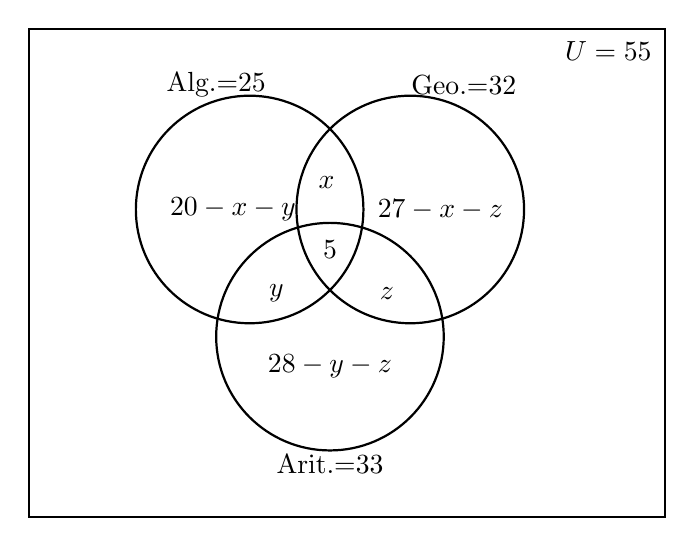
\begin{tikzpicture}[scale=0.85]
		
		% Universo
		\draw[thick] (-4.5,-3.5) rectangle (5,3.8);
		\node[anchor=north east] at (4.95,3.75) {$U=55$};
		
		% Conjuntos
		\draw[thick] (-1.2,1.1) circle (1.7);
		\draw[thick] (1.2,1.1) circle (1.7);
		\draw[thick] (0,-0.8) circle (1.7);
		
		% Etiquetas
		\node at (-1.7,2.96) {Alg.=25};
		\node at (2,2.96) {Geo.=32};
		\node at (0,-2.70) {Arit.=33};
		
		% Regiones
		\node at (-0.05,1.5) {$x$};
		\node at (-0.8,-0.15) {$y$};
		\node at (0.85,-0.15) {$z$};
		\node at (0,0.50) {$5$};
		
		\node at (-1.45,1.1) {$20-x-y$};
		\node at (1.65,1.1) {$27-x-z$};
		\node at (0,-1.25) {$28-y-z$};
		
	\end{tikzpicture}
	
	Del gráfico
	
	$25-(27-x+z)+z+(28-y-z)=55$
	
	$80-x-y-z=55$
	
	$x+y+z=25$
	
	\vspace{6mm}
	
\end{enumerate}



\subsection*{Álgebra}

\begin{enumerate}
	
	\item Halle la suma de los valores de $a$ para que la inecuación dada tenga solución única.
	
	$$x^2+(x+a)^2+2x\leq 1$$
	
	\begin{enumerate}[label=\alph*)]
		\item 1
		\item 2
		\item 3
		\item 4
		\item 5
	\end{enumerate}
	\textbf{Respuesta correcta:} b)
	
	\vspace{2mm}
	\textbf{Solucionario:}\\
	
	$2x^2+2(a+1)x+a^2-1\leq 0$
	
	$\Delta=4(a^2+2a+1)-4(2a^2-2)=0$
	
	$a^2-2a-3=0$
	
	$\therefore$ Suma $=-(-2)=2$.
	
	\vspace{6mm}
	
	\item Calcule $m\in \mathbb{N}$ si la división dada genera un cociente notable.
	
	$$\dfrac{x^{13m+1}-y^{8m+2}}{x^{m+1}-y^m}$$
	
	\begin{enumerate}[label=\alph*)]
		\item 6
		\item 4
		\item 2
		\item 1
		\item 3
	\end{enumerate}
	\textbf{Respuesta correcta:} c)
	
	\vspace{2mm}
	\textbf{Solucionario:}\\
	
	$\dfrac{13m+1}{m+1}=\dfrac{8m+2}{m}$
	
	$13m^2+m=8m^2+10m+2$
	
	$5m^2-9m-2=0$
	
	$(5m+1) y (m-2) $
	
	
	$m=-\dfrac{1}{5}\ \ \ y\ \ \fbox{m=2}$
	
	\vspace{6mm}
	
	\item La función de demanda de un artículo está dada por $x=p^2-5$ y la función de oferta está dada por $x=10-2p$, donde $x$ es la cantidad de artículos y $p$ el precio unitario. Halle el precio unitario para que el mercado esté en equilibrio.
	
	\begin{enumerate}[label=\alph*)]
		\item 3
		\item 4
		\item 5
		\item 6
		\item 7
	\end{enumerate}
	\textbf{Respuesta correcta:} a)
	
	\vspace{2mm}
	\textbf{Solucionario:}\\
	
	El mercado está en equilibrio $\Leftrightarrow$ Función de demanda $=$ Función de oferta
	
	$p^2-5=10-2p$
	
	$p^2+2p-15=0$
	
	$(p+5)(p-3)=0$
	
	$\therefore\ p=3$
	
	\vspace{6mm}
	
\end{enumerate}




\subsection*{Geometría}

\begin{enumerate}
	
	\item En la figura, si $AB=5$ y $BC=12$, calcule $r$
	
	\begin{center}
		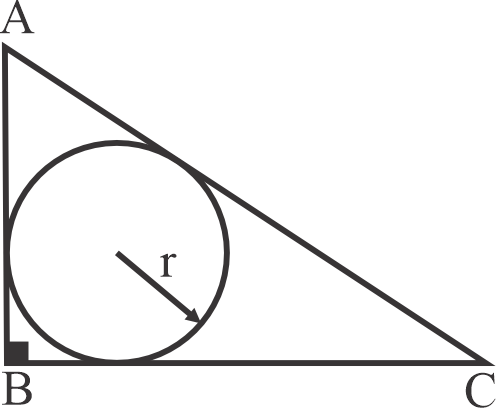
\includegraphics[width=4.5cm]{imagenes/CEPRE-UNA2024-I/etapa1/bio/geo1c24-I.png}
	\end{center}
	
	\begin{enumerate}[label=\alph*)]
		\item 5
		\item 4
		\item 3
		\item 2
		\item 1
	\end{enumerate}
	\textbf{Respuesta correcta:} d)
	
	\vspace{2mm}
	\textbf{Solucionario:}\\
	
	
	\begin{center}
		\begin{minipage}{0.45\textwidth}
			Del gráfico, por Pitágoras:
			
			$5^2+12^2=x^2 \Rightarrow x^2=169$
			
			$x=13$
			
			Por el teorema de Poncelet del gráfico:
			
			$5+12=13+2r$
			
			$17-13=2r$
			
			$4=2r$
			
			\fbox{$r=2$}
			
			\vspace{6mm}
		\end{minipage}
		\hfill
		\begin{minipage}{0.45\textwidth}
			\centering
			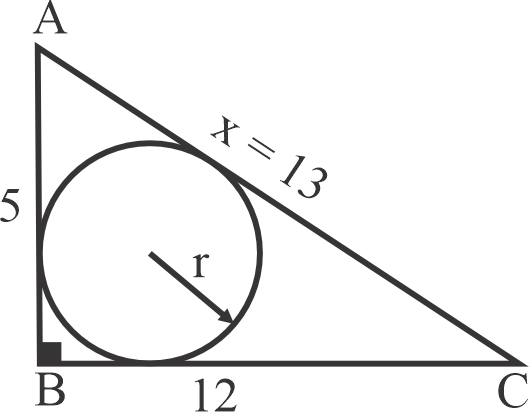
\includegraphics[width=4.5cm]{imagenes/CEPRE-UNA2024-I/etapa1/bio/geo1c24-Ir.png}
		\end{minipage}
	\end{center}
	
	\vspace{6mm}
	
	\item En el gráfico, $T$ es punto de tangencia. Calcule $2\alpha$
	
	\begin{center}
		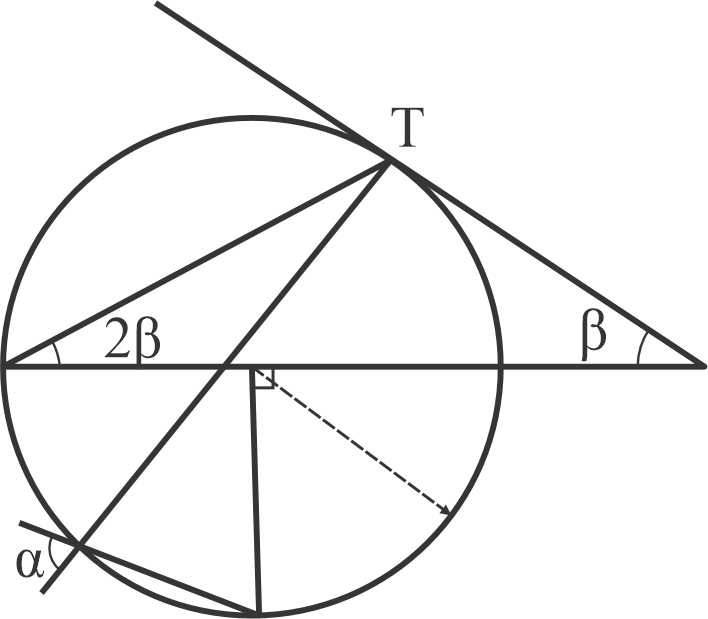
\includegraphics[width=4.2cm]{imagenes/CEPRE-UNA2024-I/etapa1/bio/geo2c24-I.png}
	\end{center}
	
	\begin{enumerate}[label=\alph*)]
		\item $162^\circ$
		\item $160^\circ$
		\item $144^\circ$
		\item $154^\circ$
		\item $132^\circ$
	\end{enumerate}
	\textbf{Respuesta correcta:} a)
	
	\vspace{2mm}
	\textbf{Solucionario:}\\
	
	
	\begin{center}
		\begin{minipage}{0.45\textwidth}
			Del triángulo $OTB$:
			
			$4\beta+\beta=90^\circ$
			
			$5\beta=90^\circ$
			
			$\beta=18^\circ$
			
			Por ángulo inscrito:
			
			$m\widehat{TKL}=2\alpha=4\beta+90^\circ$
			
			$2\alpha=4(18^\circ)+90^\circ$
			
			$2\alpha=72^\circ+90^\circ$
			
			\fbox{$2\alpha=162^\circ$}
			
			\vspace{6mm}
		\end{minipage}
		\hfill
		\begin{minipage}{0.45\textwidth}
			\centering
			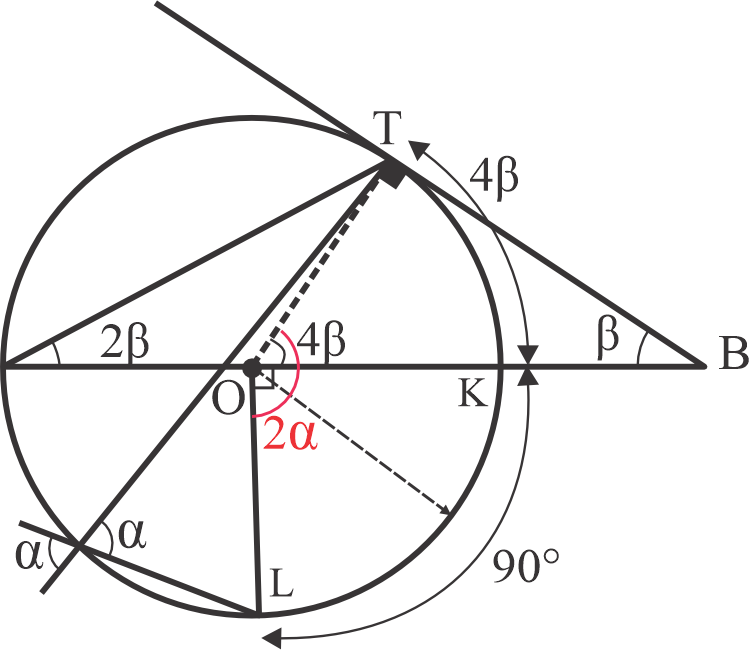
\includegraphics[width=4.5cm]{imagenes/CEPRE-UNA2024-I/etapa1/bio/geo2c24-Ir.png}
		\end{minipage}
	\end{center}
	\vspace{6mm}
	
	\item La imagen muestra un croquis de un determinado lugar. Si la Av. El Sol y la Av. La Torre son paralelas, la Av. Daniel y la Av. Francisco son paralelas, calcule $2x$.
	
	\begin{center}
		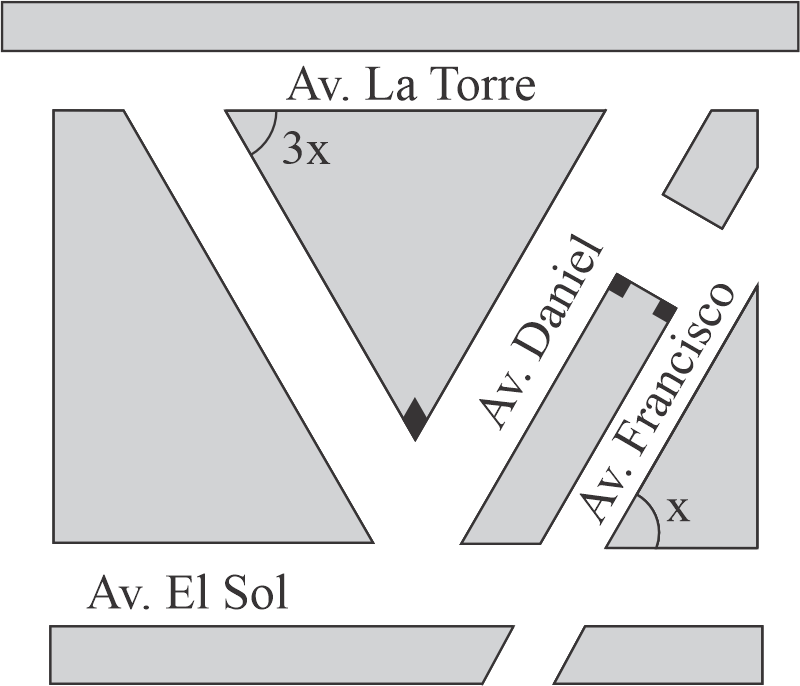
\includegraphics[width=4.5cm]{imagenes/CEPRE-UNA2024-I/etapa1/bio/geo3c24-I.png}
	\end{center}
	
	\begin{enumerate}[label=\alph*)]
		\item $60^\circ$
		\item $37^\circ$
		\item $45^\circ$
		\item $35^\circ$
		\item $30^\circ$
	\end{enumerate}
	\textbf{Respuesta correcta:} c)
	
	\vspace{2mm}
	\textbf{Solucionario:}\\
	
	\begin{center}
		\begin{minipage}{0.45\textwidth}
			Pide ``x''.
			
			Según el gráfico, la Av. Daniel y la Av. Francisco son paralelas.
			
			Del gráfico:
			
			$3x+x=90^\circ$
			
			$4x=90^\circ$
			
			\fbox{$\therefore 2x=45^\circ$}
			
			\vspace{6mm}
		\end{minipage}
		\hfill
		\begin{minipage}{0.45\textwidth}
			\centering
			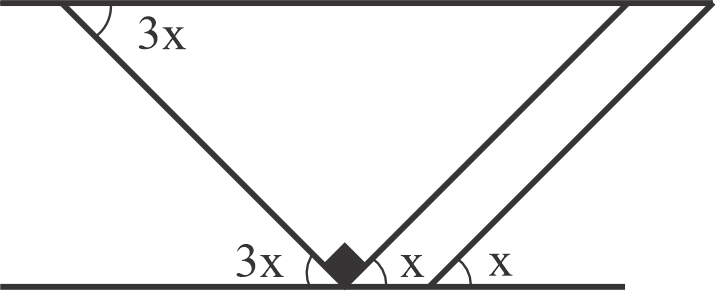
\includegraphics[width=4.5cm]{imagenes/CEPRE-UNA2024-I/etapa1/bio/geo3c24-Ir.png}
		\end{minipage}
	\end{center}
	
	
	\vspace{6mm}
	
\end{enumerate}




\subsection*{Trigonometría}

\begin{enumerate}
	
	\item En el gráfico, $ABCD$ y $AEFG$ son cuadrados, calcule $\tan\alpha+\tan\theta$
	
	\begin{center}
		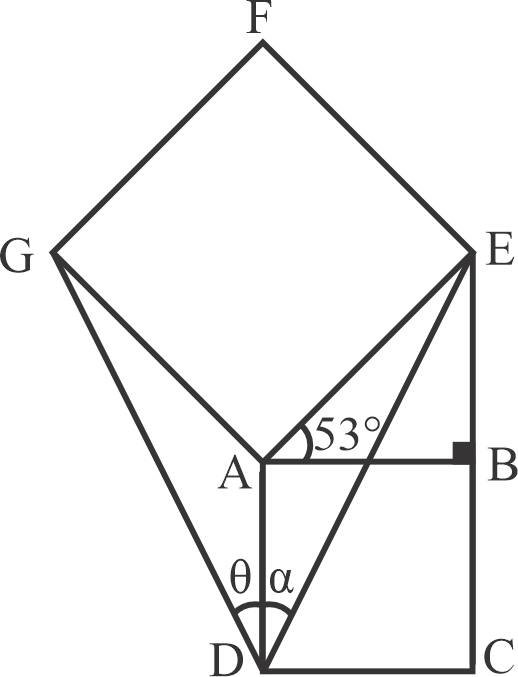
\includegraphics[width=4.5cm]{imagenes/CEPRE-UNA2024-I/etapa1/bio/trigo1c24-I.png}
	\end{center}
	
	\begin{enumerate}[label=\alph*)]
		\item $\dfrac{68}{21}$
		\item $\dfrac{67}{21}$
		\item $\dfrac{27}{8}$
		\item $\dfrac{15}{4}$
		\item $\dfrac{23}{21}$
	\end{enumerate}
	\textbf{Respuesta correcta:} e)
	
	\vspace{2mm}
	\textbf{Solucionario:}\\
	
	
	\begin{center}
		\begin{minipage}{0.45\textwidth}
			$\tan\alpha=\dfrac{3}{7};\ \tan\theta=\dfrac{4}{6}=\dfrac{2}{3}$
			
			$\therefore\ \tan\alpha+\tan\theta=\dfrac{3}{7}+\dfrac{2}{3}\\
			=\dfrac{9+14}{21}=$\fbox{$\dfrac{23}{21}$}
			
			\vspace{6mm}
		\end{minipage}
		\hfill
		\begin{minipage}{0.45\textwidth}
			\centering
			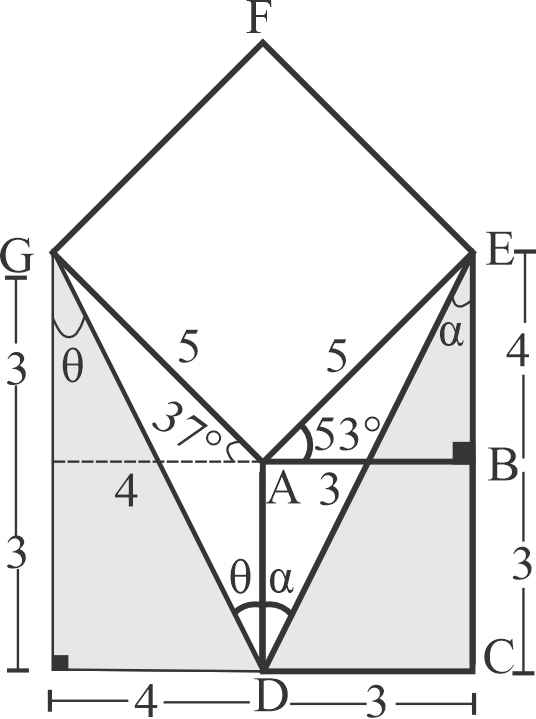
\includegraphics[width=4.5cm]{imagenes/CEPRE-UNA2024-I/etapa1/bio/trigo1c24-Ir.png}
		\end{minipage}
	\end{center}
	
	
	\vspace{6mm}
	
	\item Un estudiante de biomédicas, en vez de escribir $40^\circ$, escribe $40^g$. ¿Qué error cometió en grados sexagesimales?
	
	\begin{enumerate}[label=\alph*)]
		\item $1^\circ$
		\item $2^\circ$
		\item $3^\circ$
		\item $4^\circ$
		\item $5^\circ$
	\end{enumerate}
	\textbf{Respuesta correcta:} d)
	
	\vspace{2mm}
	\textbf{Solucionario:}\\
	
	Determinamos el error cometido:
	
	$E_{\text{error}}=\theta_{\text{verdad}}-\theta_{\text{falso}}$
	
	$=40^\circ-40^g\cdot\dfrac{9^\circ}{10^g}$
	
	$=40^\circ-4(9^\circ)$
	
	$=40^\circ-36^\circ$
	
	$E_{\text{error}}=$\fbox{$4^\circ$}
	
	\vspace{6mm}
	
	\item El perímetro de un triángulo rectángulo es $210\ m$. Si la tangente de uno de los ángulos agudos es $\dfrac{12}{5}$, calcule la longitud del cateto menor.
	
	\begin{enumerate}[label=\alph*)]
		\item $60\ m$
		\item $35\ m$
		\item $45\ m$
		\item $50\ m$
		\item $70\ m$
	\end{enumerate}
	\textbf{Respuesta correcta:} b)
	
	\vspace{2mm}
	\textbf{Solucionario:}\\
	
	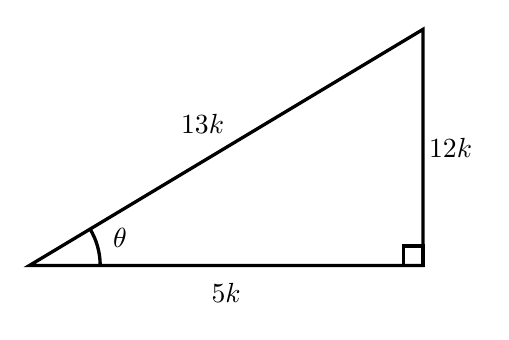
\begin{tikzpicture}[scale=1]
		
		% Triángulo
		\draw[very thick] (0,0) -- (5,0) -- (5,3) -- cycle;
		
		% Ángulo recto
		\draw[very thick] (4.75,0) rectangle (5,0.25);
		
		% Ángulo theta
		\draw[very thick] (0.9,0) arc[start angle=0,end angle=31,radius=0.9];
		\node at (1.15,0.35) {$\theta$};
		
		% Etiquetas
		\node at (2.5,-0.35) {$5k$};
		\node at (5.35,1.5) {$12k$};
		\node at (2.20,1.8) {$13k$};
		
	\end{tikzpicture}
	
	
	$\tan\theta=\dfrac{12}{5}$
	
	Perímetro:
	
	$13k+12k+5k=210$
	
	$30k=210$
	
	$k=7$
	
	Cateto menor $=5(7)$
	
	\fbox{$=35\ m$}
	
	\vspace{6mm}
	
\end{enumerate}





\subsection*{Física}

\begin{enumerate}
	
	\item Se muestra una barra homogénea de $5\ kg$ de masa en posición horizontal y articulada en el punto $A$. Si en el instante mostrado, la persona jala de la cuerda con una fuerza de $100\ N$, determine el momento de fuerza resultante sobre la barra respecto al punto $A$ para dicho instante. $(g=10\ m/s^2)$
	
	\begin{center}
		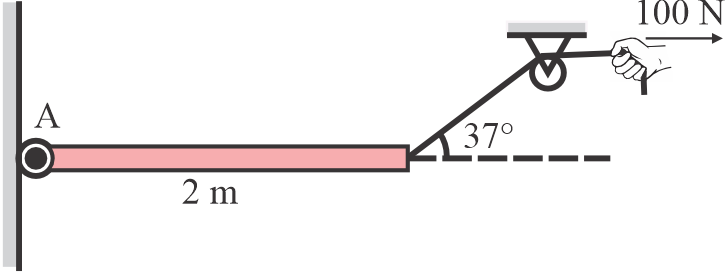
\includegraphics[width=4.5cm]{imagenes/CEPRE-UNA2024-I/etapa1/bio/fisica1c24-I.png}
	\end{center}
	
	\begin{enumerate}[label=\alph*)]
		\item $60\ \text{Nm}$
		\item $70\ \text{Nm}$
		\item $50\ \text{Nm}$
		\item $-60\ \text{Nm}$
		\item $-70\ \text{Nm}$
	\end{enumerate}
	\textbf{Respuesta correcta:} b)
	
	\vspace{2mm}
	\textbf{Solucionario:}\\
	
	
	
	\begin{center}
		\begin{minipage}{0.45\textwidth}
			$M=\dfrac{6}{5}(100)\ \text{Nm}-50\ \text{Nm}$
			
			$M=\dfrac{600}{5}\ \text{Nm}-50\ \text{Nm}$
			
			$M=120\ \text{Nm}-50\ \text{Nm}$
			
			\fbox{$M=70\ \text{Nm}$}
			
			\vspace{6mm}
		\end{minipage}
		\hfill
		\begin{minipage}{0.45\textwidth}
			\centering
			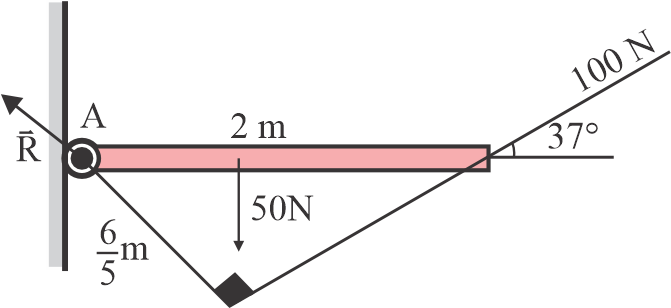
\includegraphics[width=4.5cm]{imagenes/CEPRE-UNA2024-I/etapa1/bio/fisica1c24-Ir.png}
		\end{minipage}
	\end{center}
	
	
	
	
	\vspace{6mm}
	
	\item Un cuerpo en el aire pesa $30\ N$, en el agua $25\ N$ y en un líquido desconocido $20\ N$. Halle la densidad del líquido desconocido. $(\rho_{\text{agua}}=1\ g/cm^3)$
	
	\begin{enumerate}[label=\alph*)]
		\item $1\ g/cm^3$
		\item $2\ g/cm^3$
		\item $3\ g/cm^3$
		\item $4\ g/cm^3$
		\item $5\ g/cm^3$
	\end{enumerate}
	\textbf{Respuesta correcta:} b)
	
	\vspace{2mm}
	\textbf{Solucionario:}\\
	
	\underline{Empuje en el agua} $(E)$
	
	$E=\rho_{\text{agua}}\,g\,V_{\text{cuerpo}}$
	
	$\dfrac{E}{\rho_{\text{agua}}}=gV_{\text{cuerpo}}$
	
	\underline{Empuje en el líquido desconocido} $(E')$
	
	$E'=\rho_{LD}\,g\,V_{\text{cuerpo}}$
	
	$\dfrac{E'}{\rho_{LD}}=gV_{\text{cuerpo}}$
	
	$\dfrac{E}{\rho_{\text{agua}}}=\dfrac{E'}{\rho_{LD}}$
	
	$\dfrac{30N-25N}{1000\ kg/m^3}=\dfrac{30N-20N}{\rho_{LD}}$
	
	$\dfrac{5N}{1000\ kg/m^3}=\dfrac{10N}{\rho_{LD}}$
	
	$\rho_{LD}=\dfrac{1000(10)}{5}\ kg/m^3$
	
	$\rho_{LD}=2000\ kg/m^3$
	
	\fbox{$=2\ g/cm^3$}
	
	\vspace{6mm}
	
	\item En el circuito eléctrico, determine la lectura del voltímetro y del amperímetro ideal.
	
	\begin{center}
		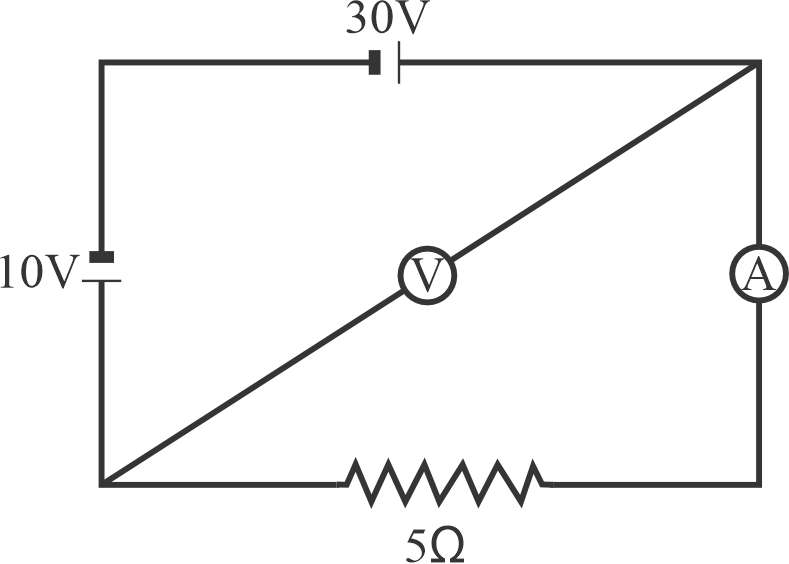
\includegraphics[width=4.5cm]{imagenes/CEPRE-UNA2024-I/etapa1/bio/fisica3c24-I.png}
	\end{center}
	
	\begin{enumerate}[label=\alph*)]
		\item $20\ V$ y $4\ A$
		\item $15\ V$ y $3\ A$
		\item $40\ V$ y $8\ A$
		\item $25\ V$ y $4\ A$
		\item $35\ V$ y $1\ A$
	\end{enumerate}
	\textbf{Respuesta correcta:} a)
	
	\vspace{2mm}
	\textbf{Solucionario:}\\
	
	Hallamos la lectura del voltímetro
	
	$\sum V=30V-10V$
	
	$V=20V$
	
	Hallamos la lectura del amperímetro ideal.
	
	$\sum V=IR$
	
	$20V=I\,5\Omega$
	
	$\dfrac{20V}{5\Omega}=I$
	
	\fbox{$4A=I$}
	
	\vspace{6mm}
	
\end{enumerate}






\subsection*{Química}

\begin{enumerate}
	
	\item Determine la cantidad de materia en $kg$ que, al descomponerse, genera $63\times 10^{20}\ Erg$ de energía.
	
	\begin{enumerate}[label=\alph*)]
		\item $8\times 10^{-2}\ Kg$
		\item $7\times 10^{-5}\ Kg$
		\item $70\ Kg$
		\item $7\times 10^{-3}\ Kg$
		\item $9\times 10^{-3}\ Kg$
	\end{enumerate}
	\textbf{Respuesta correcta:} d)
	
	\vspace{2mm}
	\textbf{Solucionario:}\\
	
	$\Delta E=\Delta m c^2$
	
	$\Delta m=\dfrac{\Delta E}{c^2}=\dfrac{63\times 10^{20}\ Erg}{(3\times 10^{10}\ cm/s)^2}$
	
	$\Delta m=\dfrac{63\times 10^{20}\ g\cdot cm^2/s^2}{9\times 10^{20}\ cm^2/s^2}$
	
	$\Delta m=7\ g\times \dfrac{1\ Kg}{10^3\ g}$
	
	\fbox{$\therefore\ \Delta m=7\times 10^{-3}\ Kg$}
	
	\vspace{6mm}
	
	\item Los alquimistas perseguían 2 propósitos: Obtener el elixir de vida (panacea) y obtener oro a partir de los elementos más baratos, los cuales no fueron logrados. Pero, ya en tiempos de la química reciente el segundo propósito se hizo realidad cuando se obtuvo el radioisótopo de oro inestable $Au-198\ (Z=79)$ a partir del bombardeo de un núcleo con 1 neutrón. Si al obtener este isótopo de oro inestable se libera un protón ¿Cuál es el núcleo bombardeado?
	
	\begin{enumerate}[label=\alph*)]
		\item $_{77}Ir$
		\item $_{78}Pt$
		\item $_{80}Hg$
		\item $_{82}Pb$
		\item $_{83}Bi$
	\end{enumerate}
	\textbf{Respuesta correcta:} c)
	
	\vspace{2mm}
	\textbf{Solucionario:}\\
	
	$^A_Z E+\,_0 n^1 \rightarrow\, _{79}Au^{198}+_1 H^1$
	
	$\Sigma Z=Z+0=79+1$
	
	\fbox{$Z=80$}
	
	\vspace{6mm}
	
	\item Al introducir una moneda de aluminio en una solución de $HCl_{(ac)}$. Se observa que se libera calor y se producen burbujas, este fenómeno se representa con la ecuación química
	
	$Al_{(s)}+HCl_{(ac)}\rightarrow AlCl_{3(ac)}+H_{2(g)}$
	
	Determine la verdad (V) o falsedad (F) de los enunciados.
	
	I. La reacción es exotérmica\\
	II. La reacción es de descomposición\\
	III. Es una reacción de simple desplazamiento
	
	\begin{enumerate}[label=\alph*)]
		\item VVV
		\item VVF
		\item VFV
		\item FVV
		\item FFV
	\end{enumerate}
	\textbf{Respuesta correcta:} c)
	
	\vspace{2mm}
	\textbf{Solucionario:}\\
	
	$Al+HCl\rightarrow AlCl_3+H_2$
	
	$2Al+6HCl\rightarrow 2AlCl_3+3H_2$
	
	$AB+C\Rightarrow AC+B$
	
	\vspace{6mm}
	
	\item ¿Cuál es la densidad del aire $(g/L)$ en la Rinconada (Puno) si la temperatura es $2^\circ C$ y la presión aproximada es $50\ cm$ de Hg? $(PM_{aire}=28,97\ g/mol\ promedio)$
	
	\begin{enumerate}[label=\alph*)]
		\item $1,1\ g/L$
		\item $0,8\ g/L$
		\item $1,0\ g/L$
		\item $0,6\ g/L$
		\item $2,0\ g/L$
	\end{enumerate}
	\textbf{Respuesta correcta:} b)
	
	\vspace{2mm}
	\textbf{Solucionario:}\\
	
	$\rho_{aire}=?$
	
	$T=2^\circ C=275^\circ K$
	
	$PM_{aire}=28,97\ g/mol$
	
	$P=50\ cm\ de\ Hg=500\ mm\ de\ Hg$
	
	$PV=nRT$
	
	$n=\dfrac{w}{PM}$
	
	$PV=\dfrac{w}{PM}RT$
	
	$P\,PM=\rho RT$
	
	$\rho=\dfrac{P\,PM}{RT}$
	
	$\rho=\dfrac{(500\ mmHg)(28,97\ g/mol)}{(62,4\ mmHg\cdot L/mol\cdot K)(275^\circ K)}=$\fbox{$0,8\ g/L$}
	
	\vspace{6mm}
	
	\item Dada la fórmula semidesarrollada del hidrocarburo:
	
	$CH_3-C(C_2H_5)(CH_3)-C(C_3H_7)(CH_3)-C(CH_3)_3$
	
	La suma de carbonos terciarios y cuaternarios es:
	
	\begin{enumerate}[label=\alph*)]
		\item 3
		\item 4
		\item 5
		\item 6
		\item 8
	\end{enumerate}
	\textbf{Respuesta correcta:} a)
	
	\vspace{2mm}
	\textbf{Solucionario:}\\
	
	Se analiza la estructura:
	
	|	$CH_3-C(C_2H_5)(CH_3)-C(C_3H_7)(CH_3)-C(CH_3)_3$
	
	Conteo:
	
	$C_1=8$
	
	$C_2=5$
	
	$C_3=0$
	
	$C_4=3$
	
	Los carbonos terciarios son aquellos unidos a $3$ carbonos, y los cuaternarios a $4$ carbonos.
	
	En la estructura dada no hay carbonos terciarios:
	
	$C_3=0$
	
	Hay $3$ carbonos cuaternarios:
	
	$C_4=3$
	
	Entonces:
	
	$C_3+C_4=0+3$
	
	$C_3+C_4=3$
	\vspace{6mm}
	
\end{enumerate}







\subsection*{Biología y Anatomía}

\begin{enumerate}
	
	\item El tejido óseo presenta células grandes y multinucleadas en una cavidad llamada Laguna de Howship. Estas células, que realizan la resorción ósea y sintetizan fosfatasa ácida, se denominan:
	\begin{enumerate}[label=\Alph*)]
		\item células osteoprogenitoras.
		\item osteoclastos.
		\item osteoblastos.
		\item osteocitos.
		\item queratinocitos.
	\end{enumerate}
	\textbf{Respuesta correcta:} b)
	
	\vspace{2mm}
	\textbf{Solucionario:}\\
	Las células que realizan la resorción ósea se ubican en las lagunas de Howship. Además, son grandes, multinucleadas y secretan enzimas como la fosfatasa ácida. Esas características corresponden a los \textbf{osteoclastos}.
	
	\vspace{6mm}
	
	\item Las meninges son membranas conectivas que envuelven y protegen al encéfalo y la médula espinal. Estas, de afuera hacia adentro, son:
	\begin{enumerate}[label=\Alph*)]
		\item piamadre, duramadre y aracnoides.
		\item seno sagital, ventrículo y duramadre.
		\item duramadre, aracnoides y piamadre.
		\item capa cerebral, cubierta y aracnoides.
		\item duramadre, cuerpo calloso y seno sagital superior.
	\end{enumerate}
	\textbf{Respuesta correcta:} c)
	
	\vspace{2mm}
	\textbf{Solucionario:}\\
	El orden anatómico correcto de las meninges, desde la más externa hasta la más interna, es:
	$ \text{duramadre} \rightarrow \text{aracnoides} \rightarrow \text{piamadre} $
	
	Por ello, la alternativa correcta es la c).
	
	\vspace{6mm}
	
	\item El ingreso del material líquido realizado por ciertos tipos de células especializadas se denomina:
	\begin{enumerate}[label=\Alph*)]
		\item exocitosis.
		\item fagocitosis.
		\item pinocitosis.
		\item ciclosis.
		\item tixotropía.
	\end{enumerate}
	\textbf{Respuesta correcta:} c)
	
	\vspace{2mm}
	\textbf{Solucionario:}\\
	Cuando la célula incorpora \textbf{líquidos} del medio, el proceso se llama \textbf{pinocitosis}.  
	La fagocitosis corresponde a la incorporación de partículas sólidas.
	
	\vspace{6mm}
	
	\item Durante la espermatogénesis, ¿en qué etapa se forman los espermatozoides a partir de las espermátidas?
	\begin{enumerate}[label=\Alph*)]
		\item Interfase
		\item Meiosis I
		\item Meiosis II
		\item Mitosis
		\item Espermiogénesis
	\end{enumerate}
	\textbf{Respuesta correcta:} e)
	
	\vspace{2mm}
	\textbf{Solucionario:}\\
	Las espermátidas se transforman en espermatozoides durante la \textbf{espermiogénesis}.  
	La meiosis I y II forman células haploides, pero la transformación final ocurre en la espermiogénesis.
	
	\vspace{6mm}
	\item Un médico explica a una madre gestante de su estado de embarazo donde le dice que está en una etapa de gemelos, para lo cual le explica que sus dos gemelos serán del mismo género, genéticamente idénticos y muy similares en su aspecto físico. Según el enunciado, ¿a qué tipo de gemelos se refiere el médico?
	\begin{enumerate}[label=\Alph*)]
		\item Fraternos
		\item Multicigóticos
		\item Digigóticos
		\item Monocigóticos
		\item Heterocigóticos
	\end{enumerate}
	\textbf{Respuesta correcta:} d)
	
	\vspace{2mm}
	\textbf{Solucionario:}\\
	Si los gemelos son del mismo sexo, genéticamente idénticos y muy parecidos físicamente, entonces proceden de un solo cigoto que luego se dividió.  
	Por eso se trata de gemelos \textbf{monocigóticos}.
	
	\vspace{6mm}
	
	\item Desarrolló experimentos para demostrar la falsedad de la generación espontánea de gusanos.
	\begin{enumerate}[label=\Alph*)]
		\item Louis Pasteur
		\item Francisco Redi
		\item John Needhan
		\item Alexander Oparin
		\item Charles Darwin
	\end{enumerate}
	\textbf{Respuesta correcta:} b)
	
	\vspace{2mm}
	\textbf{Solucionario:}\\
	Francesco Redi realizó experimentos con carne y recipientes abiertos y cerrados para demostrar que los gusanos no surgían espontáneamente, sino de huevos de moscas.  
	Por ello, la respuesta correcta es \textbf{Francisco Redi}.
	
	\vspace{6mm}
\end{enumerate}

\subsection*{Psicología y Filosofía}

\begin{enumerate}
	
	\item En un inicio, las escuelas psicológicas asumieron una postura radical sobre el objeto de estudio de la psicología, el método que deberían usar y también contribuyeron de manera notoria en su avance. Sobre el segundo punto, podemos afirmar que la Escuela Estructuralista propuso como método:
	\begin{enumerate}[label=\Alph*)]
		\item la introspección.
		\item la extrospección.
		\item el condicionamiento.
		\item los test psicológicos.
		\item el estudio de casos.
	\end{enumerate}
	\textbf{Respuesta correcta:} a)
	
	\vspace{2mm}
	\textbf{Solucionario:}\\
	La escuela estructuralista buscaba analizar la conciencia en sus elementos básicos, para lo cual empleó la \textbf{introspección}.  
	Ese fue su método principal.
	
	\vspace{6mm}
	
	\item Juan Carlos se siente muy contento porque ingresó a la universidad; por ello se siente triste por sus amigos que no ingresaron. Esto refleja claramente la característica de la afectividad denominada:
	\begin{enumerate}[label=\Alph*)]
		\item amplitud.
		\item intensidad.
		\item polaridad.
		\item intimidad.
		\item profundidad.
	\end{enumerate}
	\textbf{Respuesta correcta:} c)
	
	\vspace{2mm}
	\textbf{Solucionario:}\\
	La afectividad presenta \textbf{polaridad} porque puede manifestarse en dos sentidos opuestos, por ejemplo: alegría y tristeza.  
	En el caso planteado, Juan Carlos experimenta ambas.
	
	\vspace{6mm}
	
	\item Flora cuenta que, en el último examen de CEPRE-UNA, resolvió casi todos los problemas de matemáticas y física. Estuvo resolviendo alrededor de dos horas, ni el más leve ruido la distrajo. ¿A qué característica de la atención se refiere?
	\begin{enumerate}[label=\Alph*)]
		\item Selectiva -- distributiva
		\item Constante -- intencional
		\item Direccional -- constante
		\item Voluntaria -- refleja
		\item Selectiva -- constante
	\end{enumerate}
	\textbf{Respuesta correcta:} e)
	
	\vspace{2mm}
	\textbf{Solucionario:}\\
	Fue \textbf{selectiva} porque concentró su atención en los problemas sin distraerse por el ruido.  
	Además, fue \textbf{constante} porque mantuvo la atención durante aproximadamente dos horas.
	
	\vspace{6mm}
	
	\item Después de varios años, Rosalia vuelve a la Universidad Nacional del Altiplano, pero manifiesta que nunca ha estado en aquel lugar. El texto mencionado refiere una anomalía de memoria denominada:
	\begin{enumerate}[label=\Alph*)]
		\item hipermnesia.
		\item agnosia.
		\item amnesia.
		\item hipomnesia.
		\item paramnesia.
	\end{enumerate}
	\textbf{Respuesta correcta:} e)
	
	\vspace{2mm}
	\textbf{Solucionario:}\\
	La \textbf{paramnesia} consiste en un falso reconocimiento o distorsión del recuerdo.  
	En este caso, la persona ya estuvo allí, pero cree que nunca ha estado en ese lugar.
	
	\vspace{6mm}
	
\end{enumerate}

\subsection*{Geografía}

\begin{enumerate}
	
	
	\item El río fronterizo que limita entre Perú y Colombia es:
	\begin{enumerate}[label=\Alph*)]
		\item Putumayo.
		\item Tumbes.
		\item Chira.
		\item Amazonas.
		\item Zarumilla.
	\end{enumerate}
	\textbf{Respuesta correcta:} a)
	
	\vspace{2mm}
	\textbf{Solucionario:}\\
	El río \textbf{Putumayo} forma parte de la frontera entre Perú y Colombia.  
	Los demás corresponden a otras zonas limítrofes o no cumplen esa función específica.
	
	\vspace{6mm}
	
	\item La región natural comprendida entre los $2300$ a $3500$ m.s.n.m. se denomina:
	\begin{enumerate}[label=\Alph*)]
		\item Yunga.
		\item Chala.
		\item Suni.
		\item Puna.
		\item Quechua.
	\end{enumerate}
	\textbf{Respuesta correcta:} e)
	
	\vspace{2mm}
	\textbf{Solucionario:}\\
	Según la clasificación de Javier Pulgar Vidal, la región \textbf{Quechua} se ubica aproximadamente entre los $2300$ y $3500$ m.s.n.m.
	
	\vspace{6mm}
	
\end{enumerate}

\subsection*{Historia}

\begin{enumerate}
	
	
	\item La participación política de la mujer en el Perú se estableció con el derecho al sufragio en el gobierno de:
	\begin{enumerate}[label=\Alph*)]
		\item Alan García Pérez.
		\item José Luis Bustamante y Rivero.
		\item Manuel Arturo Odría Amoretti.
		\item Fernando Belaunde Terry.
		\item Ricardo Pérez Godoy.
	\end{enumerate}
	\textbf{Respuesta correcta:} c)
	
	\vspace{2mm}
	\textbf{Solucionario:}\\
	El derecho al sufragio femenino en el Perú fue reconocido durante el gobierno de \textbf{Manuel A. Odría}.
	
	\vspace{6mm}
	
	\item El sacrificio de Titu Kusi Huallpa, conocido como Cahuide, está relacionado con la rebelión de:
	\begin{enumerate}[label=\Alph*)]
		\item Manco Cápac.
		\item Calcu Chímac.
		\item Quisquis y Rumi Ñahui.
		\item Manco Inca.
		\item Quisu Yupanqui.
	\end{enumerate}
	\textbf{Respuesta correcta:} d)
	
	\vspace{2mm}
	\textbf{Solucionario:}\\
	Cahuide es recordado por su participación heroica en la resistencia inca durante la rebelión de \textbf{Manco Inca}.
	
	\vspace{6mm}
	
\end{enumerate}

\subsection*{Educación Cívica}

\begin{enumerate}
	
	
	\item El registro de organizaciones políticas está a cargo de:
	\begin{enumerate}[label=\Alph*)]
		\item la Oficina Nacional de Procesos Electorales.
		\item el Registro Nacional de Identificación y Estado Civil.
		\item el Jurado Nacional de Elecciones.
		\item los Jurados Electorales Especiales.
		\item el Parlamento Andino.
	\end{enumerate}
	\textbf{Respuesta correcta:} c)
	
	\vspace{2mm}
	\textbf{Solucionario:}\\
	El Registro de Organizaciones Políticas está a cargo del \textbf{Jurado Nacional de Elecciones}.
	
	\vspace{6mm}
	
	\item Dina y Martín son cuñados. ¿Cuál es el parentesco que se establece entre ellos?
	\begin{enumerate}[label=\Alph*)]
		\item Segundo grado de afinidad
		\item Primer grado de afinidad
		\item Tercer grado de consanguinidad
		\item Cuarto grado de afinidad
		\item Tercer grado de afinidad
	\end{enumerate}
	\textbf{Respuesta correcta:} a)
	
	\vspace{2mm}
	\textbf{Solucionario:}\\
	Los cuñados tienen parentesco por afinidad, no por consanguinidad.  
	Ese vínculo corresponde al \textbf{segundo grado de afinidad}.
	
	\vspace{6mm}
	
\end{enumerate}

\subsection*{Economía}

\begin{enumerate}
	
	
	\item El pan es un bien con pocos sustitutos. ¿Cómo se clasifica generalmente su elasticidad?
	\begin{enumerate}[label=\Alph*)]
		\item Demanda unitaria
		\item Demanda elástica
		\item Demanda inelástica
		\item Demanda perfectamente elástica
		\item Demanda perfectamente inelástica
	\end{enumerate}
	\textbf{Respuesta correcta:} c)
	
	\vspace{2mm}
	\textbf{Solucionario:}\\
	Si un bien tiene pocos sustitutos, la cantidad demandada no cambia mucho ante variaciones del precio.  
	Por eso su demanda suele ser \textbf{inelástica}.
	
	\vspace{6mm}
	
	\item Los tributos en el Perú se clasifican en:
	\begin{enumerate}[label=\Alph*)]
		\item tasas, contribuciones y licencias.
		\item contribuciones, tasas y derechos.
		\item arbitrios, impuestos y contribuciones.
		\item impuestos, contribuciones y tasas.
		\item licencias, contribuciones y arbitrios.
	\end{enumerate}
	\textbf{Respuesta correcta:} d)
	
	\vspace{2mm}
	\textbf{Solucionario:}\\
	La clasificación general de los tributos en el Perú es:
	$ \text{impuestos}, \text{contribuciones} \text{ y } \text{tasas} $
	
	\vspace{6mm}
	
\end{enumerate}

\subsection*{Comunicación}

\begin{enumerate}
	
	
	\item Los estudiantes de comunicación elaboraron varias diapositivas sobre el concepto, función comunicativa y estructura de los géneros periodísticos.
	
	En el acto, los estudiantes plasmaron un texto:
	\begin{enumerate}[label=\Alph*)]
		\item narrativo.
		\item expositivo.
		\item argumentativo.
		\item descriptivo.
		\item dialógico.
	\end{enumerate}
	\textbf{Respuesta correcta:} b)
	
	\vspace{2mm}
	\textbf{Solucionario:}\\
	El texto \textbf{expositivo} explica conceptos, funciones y estructuras con finalidad informativa y didáctica.  
	Eso es justamente lo que hacen las diapositivas mencionadas.
	
	\vspace{6mm}
	
	\item Un alumno comenta a su maestra sobre las dificultades que llegaron a la ciudad a raíz de la inundación en algunas calles. El alumno, en este comentario, generó un texto narrativo de tipo:
	\begin{enumerate}[label=\Alph*)]
		\item fáctico.
		\item cotidiano.
		\item ficticio.
		\item onírico.
		\item fantástico.
	\end{enumerate}
	\textbf{Respuesta correcta:} b)
	
	\vspace{2mm}
	\textbf{Solucionario:}\\
	El enunciado presenta una situación cercana a la vida diaria del estudiante, relatada dentro de un contexto real y común. Por ello, corresponde a un texto narrativo de tipo \textbf{cotidiano}.
	
	\vspace{6mm}
	
	
	\item Es la mínima unidad del habla con sentido completo. Expresa una actitud del hablante y tiene autonomía o independencia semántica y sintáctica.
	\begin{enumerate}[label=\Alph*)]
		\item La oración
		\item El verbo
		\item La morfología
		\item El sujeto
		\item La frase nominal
	\end{enumerate}
	\textbf{Respuesta correcta:} a)
	
	\vspace{2mm}
	\textbf{Solucionario:}\\
	La unidad mínima con sentido completo, autonomía y estructura sintáctica propia es la \textbf{oración}.
	
	\vspace{6mm}
	
	\item Señale la alternativa que presenta coma elíptica.
	\begin{enumerate}[label=\Alph*)]
		\item Compré chicles, caramelos, cigarrillos y chocolates.
		\item Madre, mañana viajamos.
		\item Ayer, mis padres llegaron.
		\item Mario estudia en San Ignacio de Loyola; Luis, en César Vallejo.
		\item Grau, el Héroe de los Mares, se inmoló en el Combate de Angamos.
	\end{enumerate}
	\textbf{Respuesta correcta:} d)
	
	\vspace{2mm}
	\textbf{Solucionario:}\\
	La coma elíptica sustituye un verbo omitido. En:
	$ \text{Mario estudia en San Ignacio de Loyola; Luis, en César Vallejo} $
	se omite el verbo $ \text{estudia} $ en la segunda parte.
	
	\vspace{6mm}
\end{enumerate}


\subsection*{Literatura}

\begin{enumerate}
	
	
	\item En los nudos de un tronco hacen escalas; y ensortijan sus tallos de serpientes, hasta quedar en la altitud pendiente, a manera de pájaros sin alas. Tristes como cabezas pensativas brotan ellas, sin torpes ligaduras de tirana raíz, libres y altivas.
	
	En los versos de José Santos Chocano, se aprecia como tema:
	
	\begin{enumerate}[label=\Alph*)]
		\item la identidad andina.
		\item el sincretismo cultural.
		\item el destino inevitable.
		\item el elogio a la naturaleza.
		\item la vieja oligarquía.
	\end{enumerate}
	\textbf{Respuesta correcta:} d)
	
	\vspace{2mm}
	\textbf{Solucionario:}\\
	El fragmento resalta imágenes naturales y una visión admirativa del mundo vegetal.  
	Por ello, el tema es el \textbf{elogio a la naturaleza}.
	
	\vspace{6mm}
	
	\item En la obra \textit{Divina Comedia}, Dante se pierde en una selva oscura y se enfrenta a una loba, una pantera y un león, que simbolizan respectivamente:
	\begin{enumerate}[label=\Alph*)]
		\item codicia, lujuria y soberbia.
		\item pecado, maldad y orgullo.
		\item egoísmo, ociosidad e ira.
		\item codicia, pasión y cólera.
		\item codicia, egoísmo y pasión.
	\end{enumerate}
	\textbf{Respuesta correcta:} a)
	
	\vspace{2mm}
	\textbf{Solucionario:}\\
	En la interpretación alegórica clásica de la obra:
	\begin{itemize}
		\item la loba representa la codicia,
		\item la pantera representa la lujuria,
		\item el león representa la soberbia.
	\end{itemize}
	
	\vspace{6mm}
	
\end{enumerate}

\subsection*{Razonamiento Matemático}

\begin{enumerate}
	
	\item Si cada asterisco representa una cifra, reconstruya la multiplicación e indique la suma de cifras del producto.
	
	\begin{center}
		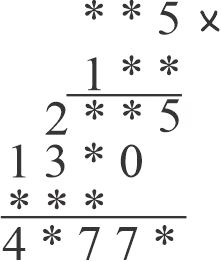
\includegraphics[width=2.5cm]{imagenes/CEPRE-UNA2024-I/etapa1/bio/rm1c24-I.png}
	\end{center}
	
	
	\begin{enumerate}[label=\Alph*)]
		\item $27$
		\item $30$
		\item $24$
		\item $29$
		\item $32$
	\end{enumerate}
	\textbf{Respuesta correcta:} b)
	
	\vspace{2mm}
	\textbf{Solucionario:}\\
	
	\begin{center}
		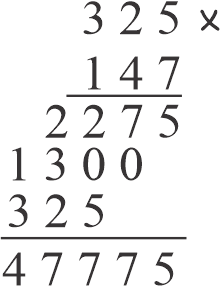
\includegraphics[width=2.5cm]{imagenes/CEPRE-UNA2024-I/etapa1/bio/rm1c24-Ir.png}
	\end{center}
	
	
	Reconstruyendo:
	
	$325\times147=47775$
	
	Piden la suma de cifras del producto, por lo tanto:
	
	$4+7+7+7+5=30$
	
	\fbox{$30$}
	
	\vspace{6mm}
	
	\item ¿Cuál es el número que completa correctamente la sucesión?
	
	$12;15;21;33;\ldots;105$
	\begin{enumerate}[label=\Alph*)]
		\item $52$
		\item $57$
		\item $60$
		\item $72$
		\item $83$
	\end{enumerate}
	\textbf{Respuesta correcta:} b)
	
	\vspace{2mm}
	\textbf{Solucionario:}\\
	
	Haciendo diferencia por cada dos términos:
	
	$15-12=3$
	
	$21-15=6$
	
	$33-21=12$
	
	Las diferencias se van duplicando.
	
	Entonces:
	
	$X-33=24$
	
	$X=24+33$
	
	$X=57$
	
	Luego:
	
	$105-57=48$
	
	$\therefore X=57$
	
	\fbox{$57$}
	
	\vspace{6mm}
	
	\item En $\mathbb{N}$, se definen los operadores:
	
	$ a \sqcup b = 2a+b $
	
	$ a \sqcap b = 2b-a $
	
	Determine el valor de $m$ en la ecuación:
	$ (4 \sqcup 3)\sqcap(2 \sqcap m)=5 $
	\begin{enumerate}[label=\Alph*)]
		\item $0$
		\item $2$
		\item $3$
		\item $4$
		\item $5$
	\end{enumerate}
	\textbf{Respuesta correcta:} d)
	
	\vspace{2mm}
	\textbf{Solucionario:}\\
	
	Empleamos las reglas de definición en cada caso.
	
	$4\sqcup3=2(4)+3=11$
	
	$2\sqcap m=2(m)-2$
	
	En lo pedido:
	
	$2(2m-2)-11=5$
	
	$4m-15=5$
	
	$4m=20$
	
	$\therefore m=5$
	
	\fbox{$5$}
	
	\vspace{1mm}
	\textbf{Observación:} la clave marcada en la pregunta original indica la alternativa d), pero con el procedimiento manuscrito proporcionado el resultado obtenido es $m=5$.
	
	\vspace{6mm}
	
	\item Cesar le dice a Elvis: ``Yo tengo la edad que tú tenías cuando yo tenía la mitad de la edad que tienes y, cuando yo tenga el doble de la edad que tú tienes, la suma de nuestras edades será $68$''. ¿Qué edad tiene Elvis?
	\begin{enumerate}[label=\Alph*)]
		\item $13$
		\item $14$
		\item $15$
		\item $16$
		\item $17$
	\end{enumerate}
	\textbf{Respuesta correcta:} d)
	
	\vspace{2mm}
	\textbf{Solucionario:}\\
	
	Planteando:
	
	\begin{center}
		\begin{tabular}{c|c|c|c}
			& Pas. & Pre. & Fut. \\
			\hline
			Cesar & $2a$ & $3a$ & $8a$ \\
			Elvis & $3a$ & $4a$ & $9a$
		\end{tabular}
	\end{center}
	
	Del enunciado:
	
	En el futuro:
	
	$8a+9a=68$
	
	Entonces $a=4$
	
	$17a=68$
	
	$a=\dfrac{68}{17}$
	
	$a=4$
	
	Por lo tanto, la edad actual de Elvis:
	
	$4a=4(4)=16$
	
	\fbox{$16$}
	
	\vspace{6mm}
	
	\item Ricardo duplica el dinero que lleva y de inmediato gasta S/ $100$. Lo que le queda vuelve a duplicarlo para luego gastar S/ $160$. Si todavía le queda S/ $80$, ¿cuánto tenía inicialmente?
	\begin{enumerate}[label=\Alph*)]
		\item $60$
		\item $100$
		\item $90$
		\item $110$
		\item $80$
	\end{enumerate}
	\textbf{Respuesta correcta:} d)
	
	\vspace{2mm}
	\textbf{Solucionario:}\\
	
	Sea $x$ el dinero que tiene Ricardo.
	
	$2(2x-100)-160=80$
	
	$4x-200-160=80$
	
	$4x-360=80$
	
	$4x=80+360$
	
	$4x=440$
	
	$x=110$
	
	\fbox{$110$}
	
	\vspace{6mm}
	
	\item Luego de varios años se encontraron Ana, Bety, Carol y Diana. Conversaron acerca de sus profesiones: química, enfermera, matemática y abogada. Ellas tienen $24$, $25$, $26$ y $27$ años.
	
	\begin{itemize}
		\item La química es la menor y prima de Ana, además saldrá con Bety.
		\item Carol no es la mayor de todas y nunca le gustaron las ciencias de la salud ni las ciencias puras.
		\item A la mayor, le encantan los números y la de ciencias de la salud tiene $25$ años.
	\end{itemize}
	
	¿Cuánto suman las edades de Diana y Carol?
	\begin{enumerate}[label=\Alph*)]
		\item $50$
		\item $51$
		\item $49$
		\item $53$
		\item $52$
	\end{enumerate}
	\textbf{Respuesta correcta:} a)
	
	\vspace{2mm}
	\textbf{Solucionario:}\\
	
	\begin{center}
		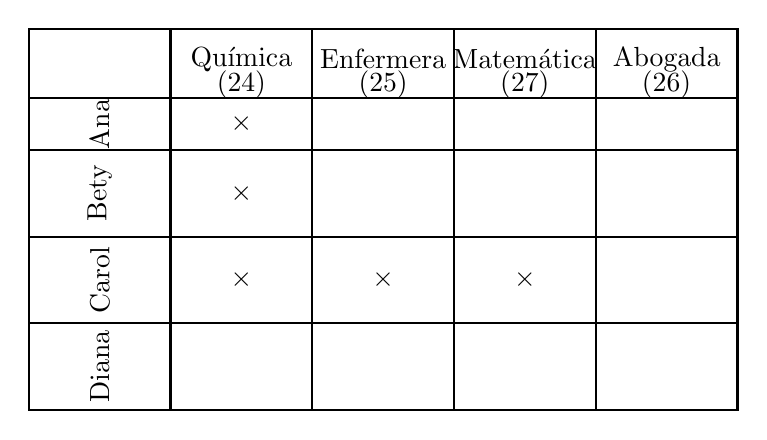
\begin{tikzpicture}[x=1.8cm,y=1.1cm]
			% marco
			\draw[thick] (0,0) rectangle (5,4.4);
			
			% divisiones verticales
			\draw[thick] (1,0) -- (1,4.4);
			\draw[thick] (2,0) -- (2,4.4);
			\draw[thick] (3,0) -- (3,4.4);
			\draw[thick] (4,0) -- (4,4.4);
			
			% divisiones horizontales
			\draw[thick] (0,1) -- (5,1);
			\draw[thick] (0,2) -- (5,2);
			\draw[thick] (0,3) -- (5,3);
			\draw[thick] (0,3.6) -- (5,3.6);
			
			% nombres laterales
			\node[rotate=90] at (0.5,3.3) {Ana};
			\node[rotate=90] at (0.5,2.5) {Bety};
			\node[rotate=90] at (0.5,1.5) {Carol};
			\node[rotate=90] at (0.5,0.5) {Diana};
			
			% encabezados
			\node at (1.5,4.05) {Química};
			\node at (2.5,4.05) {Enfermera};
			\node at (3.5,4.05) {Matemática};
			\node at (4.5,4.05) {Abogada};
			
			% edades
			\node at (1.5,3.75) {$(24)$};
			\node at (2.5,3.75) {$(25)$};
			\node at (3.5,3.75) {$(27)$};
			\node at (4.5,3.75) {$(26)$};
			
			% marcas
			\node at (1.5,3.3) {$\times$};
			
			\node at (1.5,2.5) {$\times$};
			
			\node at (1.5,1.5) {$\times$};
			\node at (2.5,1.5) {$\times$};
			\node at (3.5,1.5) {$\times$};
			\node at (4.5,1.5) {$\checkmark$};
			
			\node at (1.5,0.5) {$\checkmark$};
		\end{tikzpicture}
	\end{center}
	
	De la tabla:
	
	Diana es química y tiene $24$ años.
	
	Carol es abogada y tiene $26$ años.
	
	$\therefore 24+26=50$
	
	\fbox{$50$}
	
	\vspace{6mm}
	
\end{enumerate}

\subsection*{Razonamiento Verbal}

\begin{enumerate}
	
	
	\item La raíz y el sufijo de la palabra SINUSITIS son:
	\begin{enumerate}[label=\Alph*)]
		\item sin + usitis
		\item senos + inflamación
		\item senos + dolor
		\item sinu + sitis
		\item sinus + itis
	\end{enumerate}
	\textbf{Respuesta correcta:} e)
	
	\vspace{2mm}
	\textbf{Solucionario:}\\
	La palabra \textbf{sinusitis} se descompone en:
	\begin{itemize}
		\item raíz: \textbf{sinus}
		\item sufijo: \textbf{itis}
	\end{itemize}
	
	El sufijo \textbf{itis} indica inflamación.
	
	\vspace{6mm}
	
	\item El término excluido de QUIRÓFANO es:
	\begin{enumerate}[label=\Alph*)]
		\item bisturí.
		\item tenaza.
		\item pinza.
		\item gasa.
		\item túnica.
	\end{enumerate}
	\textbf{Respuesta correcta:} e)
	
	\vspace{2mm}
	\textbf{Solucionario:}\\
	Bisturí, tenaza, pinza y gasa son elementos relacionados con el quirófano.  
	\textbf{Túnica} no pertenece directamente a ese campo, por eso es el término excluido.
	
	\vspace{6mm}
	
	\item El antónimo de la palabra CAMELAR es:
	\begin{enumerate}[label=\Alph*)]
		\item seducir.
		\item galantear.
		\item conquistar.
		\item execrar.
		\item arrullar.
	\end{enumerate}
	\textbf{Respuesta correcta:} d)
	
	\vspace{2mm}
	\textbf{Solucionario:}\\
	\textbf{Camelar} significa enamorar, halagar o seducir.  
	Su antónimo es \textbf{execrar}, que significa aborrecer o condenar.
	
	\vspace{6mm}
	
	\item Resuelva el par analógico:
	
	VEGETAL : AUTÓTROFO ::
	\begin{enumerate}[label=\Alph*)]
		\item sapo : batracio.
		\item animal : herbívoro.
		\item hombre : omnívoro.
		\item caníbal : antropófago.
		\item pez : acuático.
	\end{enumerate}
	\textbf{Respuesta correcta:} c)
	
	\vspace{2mm}
	\textbf{Solucionario:}\\
	La relación es:
	\textbf{ser vivo} $\rightarrow$ \textbf{tipo de nutrición}
	
	Un vegetal es autótrofo.  
	De modo semejante, el hombre es omnívoro.
	
	\vspace{6mm}
	
	\item Complete la oración.
	
	Los responsables políticos pueden dar un gran paso en materia de \rule{2cm}{0.4pt}, en particular animando a desplazarse en \rule{2cm}{0.4pt}
	\begin{enumerate}[label=\Alph*)]
		\item solidaridad -- motos.
		\item salud pública -- bicicleta.
		\item apoyo ciudadano -- caminatas.
		\item servicio público -- buses.
		\item conciencia cívica -- colectivos.
	\end{enumerate}
	\textbf{Respuesta correcta:} b)
	
	\vspace{2mm}
	\textbf{Solucionario:}\\
	La expresión más coherente es:
	$ \text{salud pública} $ y $ \text{bicicleta} $
	
	Queda:
	``Los responsables políticos pueden dar un gran paso en materia de salud pública, en particular animando a desplazarse en bicicleta.''
	
	\vspace{6mm}
	
	
	
	\item PLAN DE REDACCIÓN
	
	LA ALOPATÍA
	
	I. Dichas sustancias ejercen efectos curativos sobre la zona enferma.
	
	II. Es el tratamiento de las enfermedades a través de sustancias contrarias.
	
	III. Se trata de introducir sustancias extrañas al organismo.
	
	IV. Estos efectos se producen a través de una acción bactericida.
	
	V. Alopatía viene del griego allos (otros) y phatos (enfermedades).
	
	\begin{enumerate}[label=\Alph*)]
		\item III -- IV -- I -- II -- V
		\item V -- III -- I -- IV -- II
		\item III -- I -- V -- IV -- II
		\item V -- II -- III -- IV -- I
		\item V -- II -- III -- I -- IV
	\end{enumerate}
	\textbf{Respuesta correcta:} e)
	
	\vspace{2mm}
	\textbf{Solucionario:}\\
	Primero conviene presentar el término mediante su etimología: V.  
	Luego se da la definición general: II.  
	Después se explica en qué consiste el procedimiento: III.  
	A continuación, ``dichas sustancias'' retoma a las mencionadas en III, por eso sigue I.  
	Finalmente, ``estos efectos'' retoma a los efectos curativos de I, por lo que sigue IV.
	
	Orden correcto:
	
	V -- II -- III -- I -- IV
	
	\vspace{6mm}
	
\end{enumerate}

\subsection*{Inglés}

\begin{enumerate}
	
	
	\item Complete the sentence with the correct alternative.
	
	I have pain...
	\begin{enumerate}[label=\Alph*)]
		\item dizzy.
		\item weak.
		\item in my chest.
		\item nauseous.
		\item short of breath.
	\end{enumerate}
	\textbf{Respuesta correcta:} c)
	
	\vspace{2mm}
	\textbf{Solucionario:}\\
	La expresión correcta en inglés es:
	$ \text{I have pain in my chest.} $
	
	Las demás alternativas no completan correctamente la estructura.
	
	\vspace{6mm}
	
	\item Choose the sentence which is in simple past tense.
	\begin{enumerate}[label=\Alph*)]
		\item I saw you yesterday.
		\item We are making dinner now.
		\item I will study English.
		\item They should dance in Puno.
		\item He is doing his homework.
	\end{enumerate}
	\textbf{Respuesta correcta:} a)
	
	\vspace{2mm}
	\textbf{Solucionario:}\\
	La oración en pasado simple es:
	$ \text{I saw you yesterday.} $
	
	El verbo $ \text{saw} $ es el pasado de $ \text{see} $.
	
	\vspace{6mm}
	
\end{enumerate}

\subsection*{Quechua y Aimara}

\begin{enumerate}
	\setcounter{enumi}{58}
	
	\item ¿Hayk'a chakiyuqtaq wakakuna/kanku? / Qawqha kayunisa wakaxa?
	\begin{enumerate}[label=\Alph*)]
		\item Iskay chakiyuq / Pä kayu
		\item Kimsa chakiyuq / Kimsa kayu
		\item Tawa chakiyuq / Pusi kayu
		\item Pichqa chakiyuq / Phisqa kayu
		\item Suqta chakiyuq / Suxta kayu
	\end{enumerate}
	\textbf{Respuesta correcta:} c)
	
	\vspace{2mm}
	\textbf{Solucionario:}\\
	La vaca tiene cuatro patas.
	
	En quechua:
	$ \text{tawa chakiyuq} $
	
	En aimara:
	$ \text{pusi kayu} $
	
	\vspace{6mm}
	
	\item ¿Imatataq quwikunari mikhunku? / ¿Kunsa wank'unakaxa manq'apxi?
	\begin{enumerate}[label=\Alph*)]
		\item Rumita / Qala
		\item Aquta / Ch'alla
		\item Q'achuta / Chuxlla
		\item Yakuta / Uma
		\item Alpata / Laq'a
	\end{enumerate}
	\textbf{Respuesta correcta:} c)
	
	\vspace{2mm}
	\textbf{Solucionario:}\\
	Los cuyes comen pasto o hierba.
	
	En quechua:
	$ \text{q'achuta} $
	
	En aimara:
	$ \text{chuxlla} $
	
	\vspace{6mm}
	
\end{enumerate}




\section*{Área: Sociales}



\subsection*{ Aritmética}

\begin{enumerate}
	
	\item Siendo:
	\begin{itemize}
		\item[] $p$: Américo y Jonás son hermanos
		\item[] $q$: Américo y Jonás trabajan como docentes
		\item[] $r$: Américo y Jonás son compañeros de clase de la UNA
	\end{itemize}
	
	Simbolice la proposición:
	Américo y Jonás no son hermanos ni trabajan como docentes, entonces son compañeros de clase de la UNA.
	
	\begin{enumerate}[label=\alph*)]
		\item $r \rightarrow (\sim p \wedge \sim q)$
		\item $(\sim p \wedge \sim q) \leftrightarrow r$
		\item $(\sim p \wedge \sim q) \rightarrow r$
		\item $\sim (p \wedge q) \leftrightarrow r$
		\item $\sim (p \wedge q) \rightarrow \sim r$
	\end{enumerate}
	\textbf{Respuesta correcta:} c)
	
	\vspace{2mm}
	\textbf{Solucionario:}\\
	La frase "no son hermanos ni trabajan como docentes" se traduce como la negación de ambos conectada por una conjunción: $(\sim p \wedge \sim q)$.\\
	La palabra "entonces" indica un condicional ($\rightarrow$) que apunta hacia $r$.\\
	Por lo tanto, la estructura es: $(\sim p \wedge \sim q) \rightarrow r$.
	
	\vspace{6mm}
	
	\item Un lechero ha comprado 48 litros de leche a 2.00 soles el litro. Si desea ganar 48.00 soles vendiendo a 2.40 soles el litro, ¿cuántos litros de agua debe adicionar a la leche?
	
	\begin{enumerate}[label=\alph*)]
		\item 8
		\item 4
		\item 10
		\item 5
		\item 12
	\end{enumerate}
	\textbf{Respuesta correcta:} e)
	
	\vspace{2mm}
	\textbf{Solucionario:}\\
	Ha invertido: $48 \times 2 = 96.00$ soles. \\
	Como desea ganar 48 soles, entonces la mezcla se debe vender en $96 + 48 = 144.00$ soles a razón de 2.40 soles el litro.\\
	Luego:\\
	1 litro se vende a 2.40 soles\\
	$x$ litros se vende a 144 soles\\
	$\Rightarrow x = \frac{(144)(1)}{2.4} = 60$ litros.\\
	Debe adicionar: $60 - 48 = 12$ litros.
	
	\vspace{6mm}
	
	\item ¿Cuántos múltiplos de 5 existen en el conjunto $A$?
	\[ A = \{1, 2, 3, 4, 5, \dots, 150\} \]
	
	\begin{enumerate}[label=\alph*)]
		\item 20
		\item 30
		\item 40
		\item 35
		\item 25
	\end{enumerate}
	\textbf{Respuesta correcta:} b)
	
	\vspace{2mm}
	\textbf{Solucionario:}\\
	Para hallar la cantidad de múltiplos de 5 en un conjunto de números consecutivos que empieza desde 1, se divide el último término entre 5:\\
	$n = \frac{150}{5} = 30$.\\
	Existen 30 múltiplos de 5.
	
	\vspace{6mm}
	
\end{enumerate}


\subsection*{ Álgebra}

\begin{enumerate}
	
	\item Halle el producto de los términos independientes cuando se factoriza el polinomio:
	\[ P(x) = 15x^2 + 14x - 8 \]
	
	\begin{enumerate}[label=\alph*)]
		\item 8
		\item -8
		\item 14
		\item -14
		\item 15
	\end{enumerate}
	\textbf{Respuesta correcta:} b)
	
	\vspace{2mm}
	\textbf{Solucionario:}\\
	Factorizando por aspa simple el polinomio:
	\[ 15x^2 + 14x - 8 = (5x - 2)(3x + 4) \]
	Los términos independientes de los factores son $-2$ y $4$. \\
	El producto pedido es: $(-2)(4) = $\fbox{$-8$}.
	
	\vspace{6mm}
	
	\item Halle el dominio de la función:
	\[ f(x) = \sqrt{\frac{x-1}{x-2}} \]
	
	\begin{enumerate}[label=\alph*)]
		\item $\mathbb{R} - [1,2]$
		\item $\mathbb{R} - \langle 1,2 \rangle$
		\item $\mathbb{R} - \langle 1,2 ]$
		\item $\mathbb{R} - [ 1,2 \rangle$
		\item $\langle 1,2 ]$
	\end{enumerate}
	\textbf{Respuesta correcta:} c)
	
	\vspace{2mm}
	\textbf{Solucionario:}\\
		
		Para hallar el dominio, resolvemos la inecuación:
		\[ \frac{x-1}{x-2} \geq 0 \]
		
		Puntos críticos: $1$ y $2$ ($x \neq 2$ por estar en el denominador).
		
		\begin{center}
			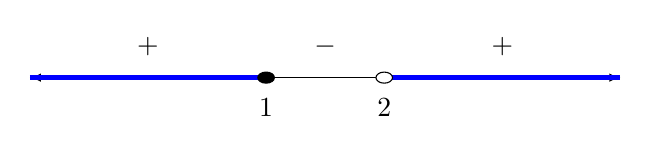
\begin{tikzpicture}[xscale=1.5]
				% Línea principal
				\draw[latex-latex] (-1,0) -- (4,0);
				
				% Regiones sombreadas
				\draw[ultra thick, blue] (-1,0) -- (1,0);
				\draw[ultra thick, blue] (2,0) -- (4,0);
				
				% Puntos críticos
				\filldraw[black] (1,0) circle (2pt) node[below=4pt] {$1$};
				\draw[black, fill=white] (2,0) circle (2pt) node[below=4pt] {$2$};
				
				% Signos
				\node at (0,0.4) {$+$};
				\node at (1.5,0.4) {$-$};
				\node at (3,0.4) {$+$};
			\end{tikzpicture}
		\end{center}
		
		$CS = \langle -\infty, 1 ] \cup \langle 2, +\infty \rangle$ \\
		\fbox{$\equiv \mathbb{R} - \langle 1, 2 ]$}

	
	\vspace{6mm}
	
	\item Halle el valor de $a$ si se sabe que $-6$ es una solución de la ecuación:
	\[ x^2 + (a+3)x + a+2 = 0 \]
	
	\begin{enumerate}[label=\alph*)]
		\item 1
		\item 2
		\item 3
		\item 4
		\item 5
	\end{enumerate}
	\textbf{Respuesta correcta:} d)
	
	\vspace{2mm}
	\textbf{Solucionario:}\\
	Reemplazamos $x = -6$:\\
	$ (-6)^2 + (a+3)(-6) + a+2 = 0 $\\
	$ 36 - 6a - 18 + a + 2 = 0 $\\
	$ 20 - 5a = 0 $\\
	$ 20 = 5a $\\
	\fbox{$ a = 4 $}\\
	
	\vspace{6mm}
	
\end{enumerate}




\subsection*{ Geometría}

\begin{enumerate}
	
	\item En el gráfico, calcule $m \angle AOB$
	
	\begin{center}
		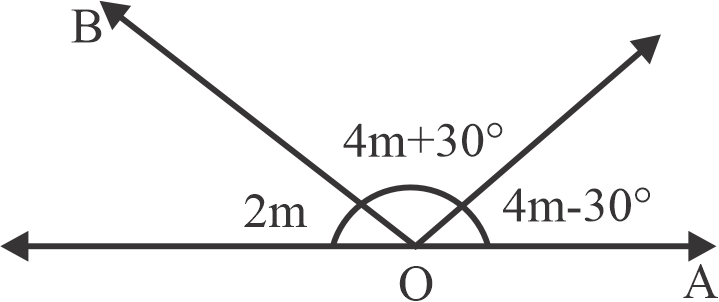
\includegraphics[width=5.5cm]{imagenes/CEPRE-UNA2024-I/etapa1/soc/geo1c24-I.png}
	\end{center}
	
	\begin{enumerate}[label=\alph*)]
		\item $144^{\circ}$
		\item $135^{\circ}$
		\item $130^{\circ}$
		\item $150^{\circ}$
		\item $162^{\circ}$
	\end{enumerate}
	\textbf{Respuesta correcta:} a)
	
	\vspace{2mm}
	\textbf{Solucionario:}\\
	Del gráfico, se tiene que la suma de los ángulos sobre la recta es $180^{\circ}$:\\
	$ 2m + 4m + 30^{\circ} + 4m - 30^{\circ} = 180^{\circ} $\\
	$ 10m = 180^{\circ} $\\
	$ m = 18^{\circ} $\\
	Piden $m \angle AOB$:\\
	$ m \angle AOB = 8m = 8(18^{\circ}) = $\fbox{$144^{\circ} $}\\
	
	\vspace{6mm}
	
	\item En la figura, $AB = BD$. Calcule $x$.
	
	\begin{center}
		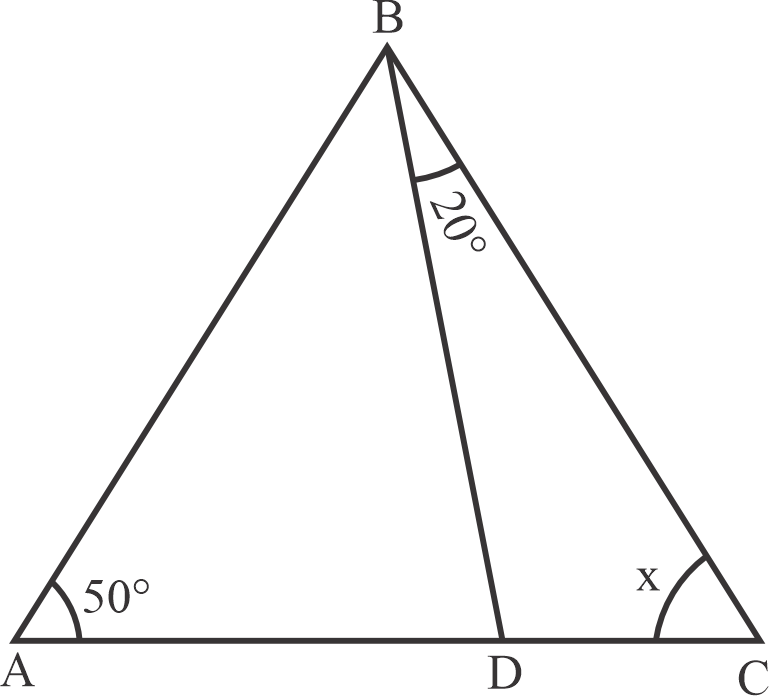
\includegraphics[width=5.5cm]{imagenes/CEPRE-UNA2024-I/etapa1/soc/geo2c24-I.png}
	\end{center}
	
	\begin{enumerate}[label=\alph*)]
		\item $20^{\circ}$
		\item $25^{\circ}$
		\item $30^{\circ}$
		\item $28^{\circ}$
		\item $35^{\circ}$
	\end{enumerate}
	\textbf{Respuesta correcta:} c)
	
	\vspace{2mm}
	\textbf{Solucionario:}\\
	
	
	
		\begin{center}
		\begin{minipage}{0.45\textwidth}
			Del gráfico:
			\begin{itemize}
				\item El $\triangle ABD$ es isósceles ($AB=BD$), de donde $m \angle BAD = m \angle BDA = 50^{\circ}$.
				\item En el $\triangle ABD$: $m \angle ABD + 50^{\circ} + 50^{\circ} = 180^{\circ} \Rightarrow m \angle ABD = 80^{\circ}$.
				\item En el $\triangle ABC$, la suma de ángulos internos es $180^{\circ}$:\\
				$ 50^{\circ} + (80^{\circ} + 20^{\circ}) + x = 180^{\circ} \\
				50^{\circ} + 100^{\circ} + x = 180^{\circ} \\
				x = 180^{\circ} - 150^{\circ} $\\
				\fbox{$x = 30^{\circ}$} 
			\end{itemize}
			
			\vspace{6mm}
		\end{minipage}
		\hfill
		\begin{minipage}{0.45\textwidth}
			\centering
			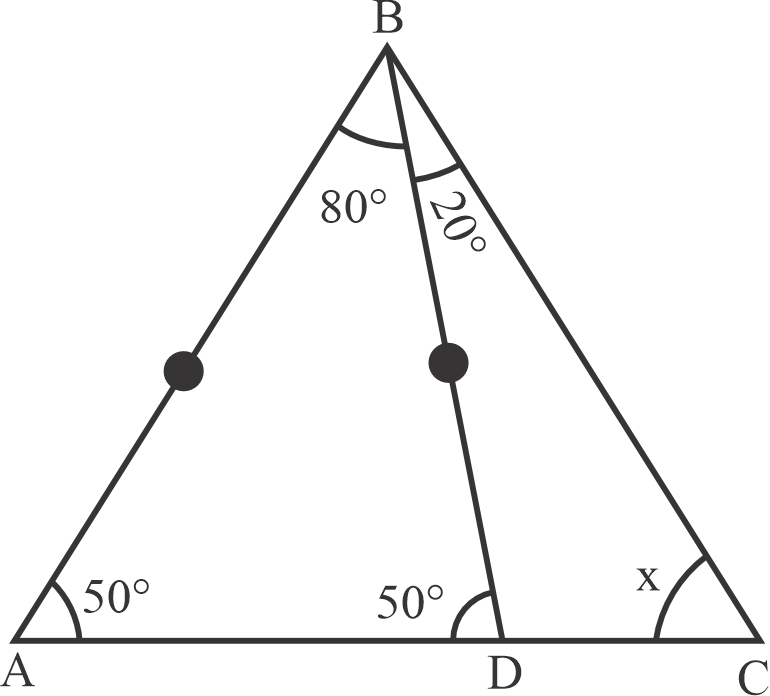
\includegraphics[width=5.5cm]{imagenes/CEPRE-UNA2024-I/etapa1/soc/geo2c24-Ir.png}
		\end{minipage}
	\end{center}
	
	\vspace{6mm}
	
\end{enumerate}







\subsection*{ Trigonometría}

\begin{enumerate}
	
	\item Calcule:
	\[ M = \sqrt{\frac{\dfrac{3\pi}{4}rad + 40^g + 29^\circ}{2^\circ}} \]
	
	\begin{enumerate}[label=\alph*)]
		\item 5
		\item 6
		\item 8
		\item 10
		\item 12
	\end{enumerate}
	\textbf{Respuesta correcta:} d)
	
	\vspace{2mm}
	\textbf{Solucionario:}\\
	Convertimos todas las unidades al sistema sexagesimal ($^\circ$):
	\begin{itemize}
		\item $\dfrac{3\pi}{4} rad \left( \dfrac{180^\circ}{\pi rad} \right) = 3(45^\circ) = 135^\circ$
		\item $40^g \left( \dfrac{9^\circ}{10^g} \right) = 4(9^\circ) = 36^\circ$
	\end{itemize}
	Reemplazando en $M$:
	\[ M = \sqrt{\frac{135^\circ + 36^\circ + 29^\circ}{2^\circ}} = \sqrt{\frac{200^\circ}{2^\circ}} = \sqrt{100} = 10 \]
	
	\vspace{6mm}
	
	\item En un triángulo rectángulo, los catetos miden $7$ y $7\sqrt{3}$ unidades. Si la hipotenusa mide $x+4$, determine $x$.
	
	\begin{enumerate}[label=\alph*)]
		\item 14
		\item 12
		\item 10
		\item 8
		\item 9
	\end{enumerate}
	\textbf{Respuesta correcta:} c)
	
	\vspace{2mm}
	\textbf{Solucionario:}\\
	Graficamos el triángulo y aplicamos el Teorema de Pitágoras:
	
	\begin{center}
		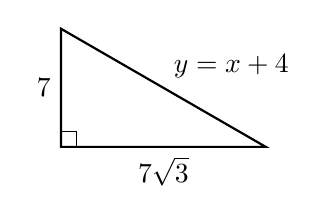
\begin{tikzpicture}[scale=0.5]
			% Triángulo recostado (Base larga en el eje X)
			\draw[thick] (0,0) -- (5.2,0) node[midway, below] {$7\sqrt{3}$} -- (0,3) node[midway, above right] {$y=x+4$} -- cycle node[midway, left] {$7$};
			% Ángulo recto
			\draw (0,0) ++(0,0.4) -- ++(0.4,0) -- ++(0,-0.4);
		\end{tikzpicture}
	\end{center}
	
	Sea $y$ la hipotenusa:\\
	$ y^2 = 7^2 + (7\sqrt{3})^2 \\
	 y^2 = 49 + 49(3) \\
	 y^2 = 49 + 147 = 196 \\
	 y = 14 $\\
	Entonces:\\
	$ y = x + 4 = 14 \\
	 x = 14 - 4 $\\
	\fbox{$ x = 10 $}
	
	\vspace{6mm}
	
\end{enumerate}






\subsection*{ Física}

\begin{enumerate}
	
	\item Si un cuerpo de $40\ N$ de peso se encuentra en equilibrio como se muestra en la figura, ¿cuál es la magnitud de la fuerza de rozamiento? ($g = 10\ m/s^2$)
	
	\begin{center}
	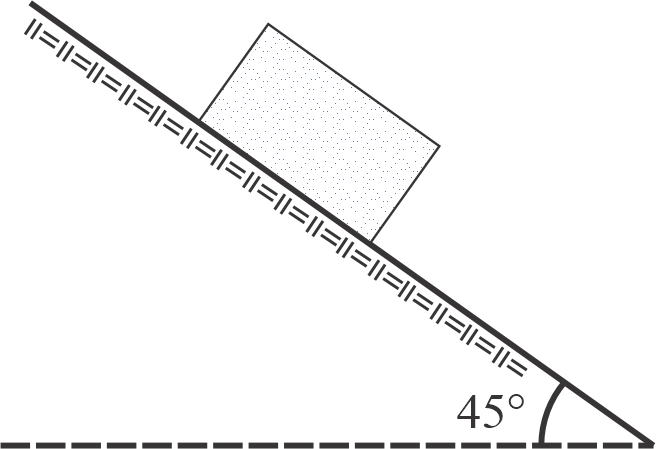
\includegraphics[width=5.5cm]{imagenes/CEPRE-UNA2024-I/etapa1/soc/fisica1c24-I.png}
	\end{center}
	
	\begin{enumerate}[label=\alph*)]
		\item $20\sqrt{2}\ N$
		\item $20\ N$
		\item $40\ N$
		\item $20\sqrt{3}\ N$
		\item $4\sqrt{3}\ N$
	\end{enumerate}
	\textbf{Respuesta correcta:} a)
	
	\vspace{2mm}
	\textbf{Solucionario:}\\
	Utilizamos el triángulo de fuerzas para un cuerpo en equilibrio en un plano inclinado:
	\begin{itemize}
		\item Peso ($W$) = $40\ N$
		\item Fuerza de rozamiento ($f_r$)
		\item Ángulo del plano = $45^\circ$
	\end{itemize}
	En el triángulo de fuerzas:
	\[ f_r = 40 \cos(45^\circ)\ N \]
	\[ f_r = 40 \left( \frac{\sqrt{2}}{2} \right)\ N \]
	\[ f_r = 20\sqrt{2}\ N \]
	
	\vspace{6mm}
	
	\item Un gran tronco de madera flota en dos líquidos diferentes, como se muestra en las figuras. Identifique la proposición correcta.
	
		\begin{center}
	\begin{minipage}{0.45\textwidth}
		\centering
		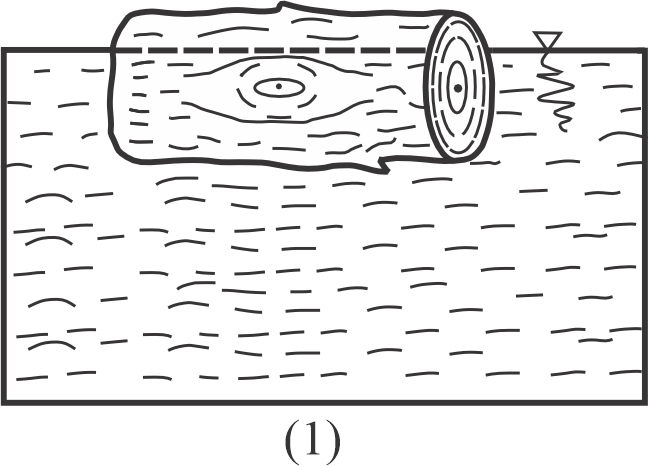
\includegraphics[width=4.5cm]{imagenes/CEPRE-UNA2024-I/etapa1/soc/fisica2c24-I.png}
		\vspace{4mm}
	\end{minipage}
	\hfill
	\begin{minipage}{0.45\textwidth}
		\centering
		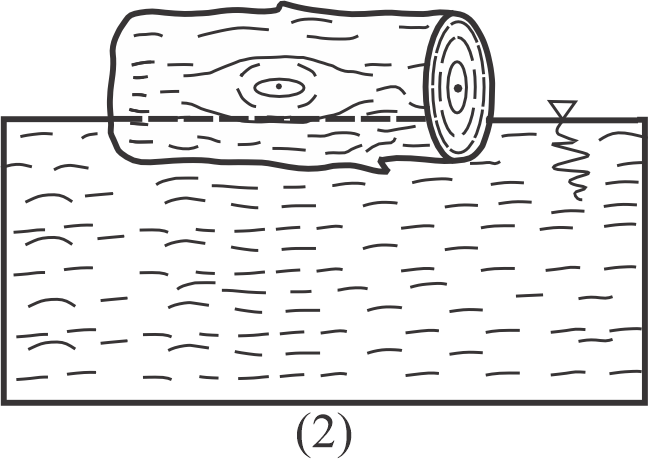
\includegraphics[width=4.5cm]{imagenes/CEPRE-UNA2024-I/etapa1/soc/fisica2c24-II.png}
	\end{minipage}
\end{center}
	
	\begin{enumerate}[label=\alph*)]
		\item El empuje en (1) es mayor que el empuje en (2)
		\item Los volúmenes de los líquidos desalojados son iguales
		\item Los líquidos tienen la misma densidad
		\item El líquido en (2) es más denso que el líquido en (1)
		\item Los empujes son iguales
	\end{enumerate}
	\textbf{Respuesta correcta:} e)
	
	\vspace{2mm}
	\textbf{Solucionario:}\\
	Como el tronco flota en ambos casos (equilibrio), se cumple que el Empuje ($E$) debe ser igual al Peso ($P$) del objeto:
	\[ E_1 = P \quad \text{y} \quad E_2 = P \]
	Por lo tanto:
	\[ E_1 = E_2 \]
	Los empujes son iguales porque en ambos casos equilibran al mismo peso del tronco.
	
	\vspace{6mm}
	
\end{enumerate}





\subsection*{Química}

\begin{enumerate}
	
	\item Respecto a la ciencia química, señale la secuencia correcta de verdad (V) o falsedad (F).
	
	I. Es la ciencia natural que estudia a la materia.\\
	II. Uno de los objetivos es la búsqueda de nuevas sustancias químicas.\\
	III. Estudia principalmente al ser humano.
	
	\begin{enumerate}[label=\alph*)]
		\item VVV
		\item VFV
		\item VVF
		\item FFF
		\item FVF
	\end{enumerate}
	\textbf{Respuesta correcta:} c)
	
	\vspace{2mm}
	\textbf{Solucionario:}\\
	I es verdadera, porque la química es la ciencia natural que estudia la materia, su composición, estructura, propiedades y transformaciones.\\
	II es verdadera, porque uno de los objetivos de la química es descubrir, analizar y sintetizar nuevas sustancias químicas.\\
	III es falsa, porque la química no estudia principalmente al ser humano, sino a la materia en general; el estudio principal del ser humano corresponde más directamente a otras ciencias como la biología.
	
	\vspace{6mm}
	
	\item Nombre el compuesto que se muestra:
	
	\[
	\mathrm{CaCO_3}
	\]
	
	\begin{enumerate}[label=\alph*)]
		\item Trióxido de calcio
		\item Tricarbono cálcico
		\item Óxido de calcio
		\item Carbonato de calcio
		\item Carbonito de calcio
	\end{enumerate}
	\textbf{Respuesta correcta:} d)
	
	\vspace{2mm}
	\textbf{Solucionario:}\\
	El compuesto \(\mathrm{CaCO_3}\) está formado por el catión calcio \(\mathrm{Ca^{2+}}\) y el anión carbonato \(\mathrm{CO_3^{2-}}\).\\
	Por ello, su nombre correcto es \textbf{carbonato de calcio}.
	
	\vspace{6mm}
	
\end{enumerate}







\subsection*{Biología y Anatomía}

\begin{enumerate}
	
	\item ¿Cuál es el ecosistema presente en las riberas de la ecorregión mar tropical del país?
	\begin{enumerate}[label=\alph*)]
		\item Desierto costero
		\item Loma costera
		\item Manglares
		\item Albúfera
		\item Bosque seco
	\end{enumerate}
	\textbf{Respuesta correcta:} c)
	
	\vspace{2mm}
	\textbf{Solucionario:}\\
	En la ecorregión del mar tropical, especialmente en la zona norte del Perú, el ecosistema característico de las riberas y zonas de transición entre agua salada y tierra son los \textbf{manglares}. Por eso, la alternativa correcta es \textbf{Manglares}.
	
	\vspace{6mm}
	
	\item Uno de los órganos vegetales más vistosos y atractivos son las flores de las plantas angiospermas. Sus pétalos presentan variedad de formas y colores. Señale la organela que abunda en las células de esta estructura floral.
	\begin{enumerate}[label=\alph*)]
		\item Cromoplastos
		\item Vacuolas
		\item Cloroplastos
		\item Tilacoides
		\item Pared celular
	\end{enumerate}
	\textbf{Respuesta correcta:} a)
	
	\vspace{2mm}
	\textbf{Solucionario:}\\
	Los pétalos presentan colores vistosos debido a la presencia de pigmentos carotenoides almacenados en los \textbf{cromoplastos}. Estas organelas se especializan en dar color a flores y frutos. Por eso, la respuesta correcta es \textbf{cromoplastos}.
	
	\vspace{6mm}
	
\end{enumerate}

\subsection*{Psicología y Filosofía}

\begin{enumerate}
	
	\item El enunciado socrático: ``solo sé que nada sé'' hace referencia a:
	\begin{enumerate}[label=\alph*)]
		\item la construcción del paradigma científico.
		\item la importancia de las paradojas.
		\item la limitación del conocimiento humano.
		\item la trascendencia de la ciencia griega.
		\item la imposibilidad de la filosofía.
	\end{enumerate}
	\textbf{Respuesta correcta:} c)
	
	\vspace{2mm}
	\textbf{Solucionario:}\\
	La frase socrática expresa humildad intelectual: reconoce que el ser humano tiene un conocimiento limitado. No afirma que sea imposible conocer, sino que invita a la búsqueda crítica de la verdad. Por ello, la respuesta correcta es \textbf{la limitación del conocimiento humano}.
	
	\vspace{6mm}
	
	\item La respuesta tentativa a la solución de un problema es:
	\begin{enumerate}[label=\alph*)]
		\item la verificación.
		\item la demostración.
		\item la contrastación.
		\item la hipótesis.
		\item la teoría científica.
	\end{enumerate}
	\textbf{Respuesta correcta:} d)
	
	\vspace{2mm}
	\textbf{Solucionario:}\\
	En el método científico, una explicación o respuesta provisional frente a un problema se denomina \textbf{hipótesis}. Luego esa hipótesis será comprobada, verificada o contrastada. Por eso, la respuesta es \textbf{la hipótesis}.
	
	\vspace{6mm}
	
	\item Si ponemos una cuchara en un vaso transparente con agua, la vemos como si estuviese doblada o partida cuando en realidad no lo está. Esta alteración de la percepción se denomina:
	\begin{enumerate}[label=\alph*)]
		\item alucinación.
		\item ilusión subjetiva.
		\item alomnesia.
		\item ilusión objetiva.
		\item paramnesia.
	\end{enumerate}
	\textbf{Respuesta correcta:} d)
	
	\vspace{2mm}
	\textbf{Solucionario:}\\
	La cuchara no está doblada realmente; la percepción se altera por un estímulo externo real, en este caso por la refracción de la luz en el agua. Eso corresponde a una \textbf{ilusión objetiva}. No es alucinación, porque sí existe un objeto real.
	
	\vspace{6mm}
	
	\item Raúl es una persona que tiene una necesidad incontrolada de querer dormir. Esta alteración se denomina:
	\begin{enumerate}[label=\alph*)]
		\item insomnio.
		\item narcolepsia.
		\item hipersomnia.
		\item apneas de sueño.
		\item pesadillas.
	\end{enumerate}
	\textbf{Respuesta correcta:} c)
	
	\vspace{2mm}
	\textbf{Solucionario:}\\
	La \textbf{hipersomnia} es un trastorno caracterizado por somnolencia excesiva y una necesidad anormal de dormir durante el día o por periodos prolongados.\\

	
	\vspace{6mm}
	
\end{enumerate}

\subsection*{Geografía}

\begin{enumerate}
	
	\item Es la suma de recursos materiales y humanos de una nación que aún no se aprovecha ni se explota racionalmente. Se mantiene en reserva para el futuro de su población.
	\begin{enumerate}[label=\alph*)]
		\item La realidad nacional
		\item El poder nacional
		\item El potencial nacional
		\item La política nacional
		\item El acuerdo nacional
	\end{enumerate}
	\textbf{Respuesta correcta:} c)
	
	\vspace{2mm}
	\textbf{Solucionario:}\\
	El \textbf{potencial nacional} está formado por los recursos humanos y materiales disponibles que todavía no se aprovechan plenamente, pero que pueden servir para el desarrollo futuro del país.
	
	\vspace{6mm}
	
	\item Las auroras polares o boreales, visibles en zonas cercanas a los polos, están ubicadas en la:
	\begin{enumerate}[label=\alph*)]
		\item mesósfera.
		\item ionósfera.
		\item estratósfera.
		\item tropósfera.
		\item exósfera.
	\end{enumerate}
	\textbf{Respuesta correcta:} b)
	
	\vspace{2mm}
	\textbf{Solucionario:}\\
	Las auroras se producen por la interacción de partículas solares con gases de las capas altas de la atmósfera, especialmente en la \textbf{ionósfera}. Por eso, la alternativa correcta es \textbf{ionósfera}.
	
	\vspace{6mm}
	
	\item La relación que existe entre las dimensiones de lo representado en un mapa y la distancia real se denomina:
	\begin{enumerate}[label=\alph*)]
		\item proyección.
		\item simbología.
		\item leyenda.
		\item mapa.
		\item escala.
	\end{enumerate}
	\textbf{Respuesta correcta:} e)
	
	\vspace{2mm}
	\textbf{Solucionario:}\\
	La \textbf{escala} expresa la proporción entre una distancia en el mapa y su correspondiente distancia real en el terreno. Es un elemento fundamental de la cartografía.
	
	\vspace{6mm}
	
	\item Son depresiones profundas y verticales de paredes estrechas formadas por erosión fluvial.
	\begin{enumerate}[label=\alph*)]
		\item Volcanes
		\item Mesetas
		\item Cañones
		\item Valles interandinos
		\item Pasos o abras
	\end{enumerate}
	\textbf{Respuesta correcta:} c)
	
	\vspace{2mm}
	\textbf{Solucionario:}\\
	Los \textbf{cañones} son formas de relieve profundas, estrechas y de paredes escarpadas, originadas principalmente por la erosión de los ríos a lo largo del tiempo.
	
	\vspace{6mm}
	
\end{enumerate}

\subsection*{Historia}

\begin{enumerate}
	
	\item Los restos humanos (fósiles) más antiguos hallados en la costa corresponden al hombre de:
	\begin{enumerate}[label=\alph*)]
		\item Paiján.
		\item Siches.
		\item Lauricocha.
		\item Chivateros.
		\item Paccaicasa.
	\end{enumerate}
	\textbf{Respuesta correcta:} a)
	
	\vspace{2mm}
	\textbf{Solucionario:}\\
	El \textbf{hombre de Paiján} corresponde a uno de los restos humanos más antiguos encontrados en la costa peruana. Lauricocha pertenece a la sierra, mientras que Chivateros es más conocido por su industria lítica.
	
	\vspace{6mm}
	
	\item La consecuencia de la nacionalización del salitre durante el gobierno de Manuel Pardo y Lavalle fue:
	\begin{enumerate}[label=\alph*)]
		\item la recuperación explosiva de la estabilidad económica.
		\item el despegue del capitalismo industrial peruano.
		\item el perjuicio a las empresas salitreras del capitalismo anglochileno.
		\item la férrea oposición de la burguesía boliviana.
		\item el incremento de los precios del guano.
	\end{enumerate}
	\textbf{Respuesta correcta:} c)
	
	\vspace{2mm}
	\textbf{Solucionario:}\\
	La política de nacionalización del salitre afectó los intereses de compañías extranjeras vinculadas al capital anglochileno. Por eso, una de sus consecuencias fue el \textbf{perjuicio a las empresas salitreras del capitalismo anglochileno}.
	
	\vspace{6mm}
	
	\item Eran los jefes de cada ayllu quienes servían de intermediarios entre el Estado inca y las etnias para asegurar la producción y la disposición de la mano de obra de los hatunrunas en la mita.
	\begin{enumerate}[label=\alph*)]
		\item Tucuy Ricuq
		\item Apunchik
		\item Camachic
		\item Apuquispay
		\item Curacas
	\end{enumerate}
	\textbf{Respuesta correcta:} e)
	
	\vspace{2mm}
	\textbf{Solucionario:}\\
	Los \textbf{curacas} eran los jefes locales de los ayllus y actuaban como intermediarios entre la autoridad incaica y la población. Cumplían funciones administrativas, productivas y de organización del trabajo.
	
	\vspace{6mm}
	
	\item Es una institución colegiada conformada por varios miembros que gobernó desde España las colonias en América.
	\begin{enumerate}[label=\alph*)]
		\item La Casa de Contratación de Sevilla
		\item La Cámara de Comunes
		\item La Casa Real de España
		\item El Consejo de los Austrias
		\item El Real y Supremo Consejo de Indias
	\end{enumerate}
	\textbf{Respuesta correcta:} e)
	
	\vspace{2mm}
	\textbf{Solucionario:}\\
	El órgano encargado de asesorar al rey y dirigir los asuntos de las colonias americanas fue el \textbf{Real y Supremo Consejo de Indias}. La Casa de Contratación cumplía sobre todo funciones comerciales y de control del tráfico con América.
	
	\vspace{6mm}
	
\end{enumerate}

\subsection*{Educación Cívica}

\begin{enumerate}
	
	\item María Elena tiene un hijo llamado Javier. El padre se niega a pasar una pensión de alimentos. María Elena piensa recurrir al Poder Judicial para solicitar la pensión de alimentos. Pero ella sabe que recurrir a un proceso judicial demanda tiempo y dinero. ¿Qué otra alternativa tiene María Elena para pedir la pensión de alimentos?
	\begin{enumerate}[label=\alph*)]
		\item Negación
		\item Mediación
		\item Arbitraje
		\item Conciliación
		\item Juicio
	\end{enumerate}
	\textbf{Respuesta correcta:} d)
	
	\vspace{2mm}
	\textbf{Solucionario:}\\
	Antes de iniciar un proceso judicial, en muchos casos puede acudirse a la \textbf{conciliación}, que busca que las partes lleguen a un acuerdo de forma más rápida y menos costosa.
	
	\vspace{6mm}
	
	\item Martha y David son novios. Se encuentran perdidamente enamorados. Y después de 5 años de relación deciden hacer una promesa en la cual pactan la fecha indicada para llevar adelante su matrimonio civil. ¿Qué figura civil suscribirán los novios?
	\begin{enumerate}[label=\alph*)]
		\item Esponsales
		\item Concejo de familia
		\item Pre contrato
		\item Unión de hecho
		\item Compromiso civil
	\end{enumerate}
	\textbf{Respuesta correcta:} a)
	
	\vspace{2mm}
	\textbf{Solucionario:}\\
	La promesa recíproca de matrimonio se denomina \textbf{esponsales}. No equivale al matrimonio mismo, sino al compromiso formal de celebrarlo posteriormente.
	
	\vspace{6mm}
	
	\item Richar, antes de su fallecimiento, mediante un testamento, deja su voluntad expresa de sus bienes, la misma que ha sido declarada nulo. ¿De qué manera sus herederos pedirán la transmisión de sus bienes y derechos?
	\begin{enumerate}[label=\alph*)]
		\item Sucesión intestada
		\item Sucesión voluntaria
		\item Sucesión de bienes
		\item Sucesión testamentaria
		\item Mediante un albacea
	\end{enumerate}
	\textbf{Respuesta correcta:} a)
	
	\vspace{2mm}
	\textbf{Solucionario:}\\
	Si el testamento ha sido declarado nulo, ya no produce efectos jurídicos. En ese caso, la transmisión de los bienes se realiza mediante \textbf{sucesión intestada}.
	
	\vspace{6mm}
	
	\item La aprobación de la cuenta general de la república es una atribución de:
	\begin{enumerate}[label=\alph*)]
		\item la Comisión Permanente.
		\item el Congreso de la República.
		\item la Defensoría del Pueblo.
		\item la Cámara de Senadores.
		\item la Fiscalía de la Nación.
	\end{enumerate}
	\textbf{Respuesta correcta:} b)
	
	\vspace{2mm}
	\textbf{Solucionario:}\\
	En el Perú, la \textbf{Cuenta General de la República} es revisada y aprobada por el \textbf{Congreso de la República}, que ejerce control sobre las finanzas públicas.
	
	\vspace{6mm}
	
\end{enumerate}

\subsection*{Economía}

\begin{enumerate}
	
	\item En el Perú, la institución responsable de la elaboración de la balanza de pagos es:
	\begin{enumerate}[label=\alph*)]
		\item Ministerio de Economía.
		\item Banco de la Nación.
		\item Banco Central de Reserva.
		\item Banco Financiero.
		\item Banco Agrario.
	\end{enumerate}
	\textbf{Respuesta correcta:} c)
	
	\vspace{2mm}
	\textbf{Solucionario:}\\
	La \textbf{balanza de pagos} del Perú es elaborada por el \textbf{Banco Central de Reserva del Perú (BCRP)}, porque esta institución registra y analiza las operaciones económicas del país con el exterior.
	
	\vspace{6mm}
	
	\item Si un país experimenta una devaluación de su moneda, ¿cuál de las afirmaciones es correcta en relación con el tipo de cambio?
	\begin{enumerate}[label=\alph*)]
		\item El tipo de cambio aumenta.
		\item El tipo de cambio disminuye.
		\item El tipo de cambio es constante.
		\item El tipo de cambio es flexible.
		\item El tipo de cambio depende de la oferta.
	\end{enumerate}
	\textbf{Respuesta correcta:} a)
	
	\vspace{2mm}
	\textbf{Solucionario:}\\
	Si la moneda nacional se devalúa, se necesita una mayor cantidad de moneda nacional para obtener una unidad de moneda extranjera. Por ello, \textbf{el tipo de cambio aumenta}.
	
	\vspace{6mm}
	
	\item Arturo, en una reunión social, perdió su Documento Nacional de Identidad (DNI), por lo que decide solicitar su duplicado. ¿Qué tributo deberá pagar?
	\begin{enumerate}[label=\alph*)]
		\item Multa
		\item Tasa
		\item Derecho
		\item Arbitrio
		\item Contribución
	\end{enumerate}
	\textbf{Respuesta correcta:} b)
	
	\vspace{2mm}
	\textbf{Solucionario:}\\
	El pago que se realiza por recibir un servicio administrativo individualizado del Estado, como el duplicado del DNI, es una \textbf{tasa}. No es multa ni contribución.
	
	\vspace{6mm}
	
	\item Julia es propietaria de una vivienda ubicada en la ciudad de Juliaca. ¿Cuál de los impuestos locales debe pagar anualmente?
	\begin{enumerate}[label=\alph*)]
		\item Impuesto a los bienes muebles
		\item Impuesto Selectivo al Consumo
		\item Impuesto al Rodaje
		\item Impuesto Predial
		\item Impuesto de Alcabala
	\end{enumerate}
	\textbf{Respuesta correcta:} d)
	
	\vspace{2mm}
	\textbf{Solucionario:}\\
	El tributo municipal que grava la propiedad de los inmuebles urbanos o rústicos es el \textbf{Impuesto Predial}, el cual se paga periódicamente por los propietarios.
	
	\vspace{6mm}
	
\end{enumerate}

\subsection*{Comunicación}

\begin{enumerate}
	
	\item Un joven llega a una ciudad y observa en algunas paredes textos escritos en español e inglés; de igual forma contempla avisos publicitarios con imágenes de conflictos sociales. ¿En qué categoría del sistema comunicativo se describe la experiencia del joven?
	\begin{enumerate}[label=\alph*)]
		\item Lenguaje
		\item Lengua
		\item Habla
		\item Dialecto
		\item Jerga
	\end{enumerate}
	\textbf{Respuesta correcta:} a)
	
	\vspace{2mm}
	\textbf{Solucionario:}\\
	La experiencia descrita incluye signos verbales y no verbales: textos en distintos idiomas e imágenes publicitarias. Eso corresponde al \textbf{lenguaje}, entendido como el sistema general de comunicación mediante signos.
	
	\vspace{6mm}
	
	\item Yo utilizo mi celular para tomar notas ella una libreta. La oración requiere:
	\begin{enumerate}[label=\alph*)]
		\item 1 coma -- 1 punto y seguido.
		\item 1 punto y coma -- 1 coma.
		\item 1 punto y coma -- 2 puntos.
		\item 1 punto -- 1 punto y coma.
		\item 2 puntos -- comas.
	\end{enumerate}
	\textbf{Respuesta correcta:} b)
	
	\vspace{2mm}
	\textbf{Solucionario:}\\
	La forma correcta sería: \textit{Yo utilizo mi celular para tomar notas; ella, una libreta}.\\
	Se requiere \textbf{un punto y coma} para separar dos proposiciones relacionadas y \textbf{una coma} para marcar la elipsis verbal.
	
	\vspace{6mm}
	
	\item No podrás convencer... si tú no ... das seguridad; anima... porque es tu hija. Complete con pronombres átonos.
	\begin{enumerate}[label=\alph*)]
		\item lo -- le -- lo
		\item lo -- le -- la
		\item la -- la -- la
		\item le -- le -- le
		\item la -- le -- la
	\end{enumerate}
	\textbf{Respuesta correcta:} e)
	
	\vspace{2mm}
	\textbf{Solucionario:}\\
	La oración correcta es: \textit{No podrás convencerla si tú no le das seguridad; anímala porque es tu hija}.\\
	Por tanto, la secuencia es \textbf{la -- le -- la}.
	
	\vspace{6mm}
	
	\item Una maestra ejemplifica los géneros periodísticos frente a sus estudiantes. En el proceso, les explica que una editorial periodística corresponde a un texto:
	\begin{enumerate}[label=\alph*)]
		\item descriptivo.
		\item expositivo.
		\item argumentativo.
		\item narrativo.
		\item dialógico.
	\end{enumerate}
	\textbf{Respuesta correcta:} c)
	
	\vspace{2mm}
	\textbf{Solucionario:}\\
	La \textbf{editorial} expresa una postura u opinión institucional sobre un tema y busca persuadir al lector mediante razones. Por eso corresponde a un texto \textbf{argumentativo}.
	
	\vspace{6mm}
	
\end{enumerate}

\subsection*{Literatura}

\begin{enumerate}
	
	\item ``Era un jardín sonriente, / era una tranquila fuente de cristal, / era a su borde asomada, / una rosa inmaculada del rosal''.\\
	Los versos anteriores contienen la figura literaria:
	\begin{enumerate}[label=\alph*)]
		\item epífora.
		\item complexión.
		\item anáfora.
		\item retruécano.
		\item reduplicación.
	\end{enumerate}
	\textbf{Respuesta correcta:} c)
	
	\vspace{2mm}
	\textbf{Solucionario:}\\
	La palabra \textit{era} se repite al inicio de varios versos. Esa repetición al comienzo de unidades sintácticas o versos se denomina \textbf{anáfora}.
	
	\vspace{6mm}
	
	\item En la novela \textit{Cien Años de Soledad} de Gabriel García Márquez, los fundadores de la familia son los primos José Arcadio Buendía y Úrsula Iguarán, quienes se casan pese al temor de su parentesco y terrible augurio como:
	\begin{enumerate}[label=\alph*)]
		\item el nacimiento de un niño con cola de cerdo.
		\item la muerte de la madre a manos del hijo.
		\item la destrucción del pueblo Macondo.
		\item la guerra civil causada por este matrimonio.
		\item la soledad de la familia durante cien años.
	\end{enumerate}
	\textbf{Respuesta correcta:} a)
	
	\vspace{2mm}
	\textbf{Solucionario:}\\
	En la novela existe el temor de que, por el parentesco entre los esposos, nazca un hijo con \textbf{cola de cerdo}. Ese es el augurio que acompaña a la familia Buendía.
	
	\vspace{6mm}
	
	\item Es una novela de crítica social del autor cuyo argumento y personajes han sido adecuados al mensaje político de liberación nacional y reivindicaciones sociales y económicas que crean condiciones reales y efectivas de igualdad, inclusión y justicia social.
	\begin{enumerate}[label=\alph*)]
		\item España, aparta de mí este cáliz
		\item Trilce
		\item Poemas humanos
		\item Tungsteno
		\item Sermón de la barbarie
	\end{enumerate}
	\textbf{Respuesta correcta:} d)
	
	\vspace{2mm}
	\textbf{Solucionario:}\\
	\textbf{Tungsteno}, de César Vallejo, es una novela de clara denuncia social y crítica a la explotación y a las desigualdades económicas. Por eso, la respuesta correcta es \textbf{Tungsteno}.
	
	\vspace{6mm}
	
	\item Miguel de Cervantes Saavedra, ilustre novelista, dramaturgo y poeta, se lamenta de su falta de talento poético: ``Yo que siempre me afano y me desvelo / por parecer que tengo de poeta / la gracia que no quiso darme el cielo...''\\
	Estos versos corresponden al poema:
	\begin{enumerate}[label=\alph*)]
		\item El viaje al Parnaso
		\item Epístola a Mateo Vázquez
		\item El canto a Calíope
		\item A un ermitaño
		\item Dos canciones a la Armada Invencible
	\end{enumerate}
	\textbf{Respuesta correcta:} a)
	
	\vspace{2mm}
	\textbf{Solucionario:}\\
	Los versos citados pertenecen a \textbf{El viaje al Parnaso}, obra en la que Cervantes reflexiona sobre la poesía y su propia condición de poeta.
	
	\vspace{6mm}
	
\end{enumerate}

\subsection*{Razonamiento Matemático}

\begin{enumerate}
	
	\item Indique el valor de \(x\) en la analogía:
	\[
	13\ (32)\ 26
	\]
	\[
	57\ (24)\ 20
	\]
	\[
	62\ (x)\ 51
	\]
	\begin{enumerate}[label=\alph*)]
		\item 64
		\item 48
		\item 32
		\item 24
		\item 18
	\end{enumerate}
	\textbf{Respuesta correcta:} b)
	
	\vspace{2mm}
	\textbf{Solucionario:}\\
	Se observa la regla:
	\[
	(\text{suma de cifras del primer número}) \times (\text{suma de cifras del tercer número})
	\]
	Primer caso:
	\[
	(1+3)(2+6)=4\times 8=32
	\]
	Segundo caso:
	\[
	(5+7)(2+0)=12\times 2=24
	\]
	Tercer caso:
	\[
	(6+2)(5+1)=8\times 6=48
	\]
	Por tanto, \(\boxed{x=48}\).
	
	\vspace{6mm}
	
	\item Si Jhon es nieto del papá de Jaime que tiene 10 años y Jaime tiene como único cuñado a Pedro. ¿Qué viene a ser la esposa de Pedro respecto a Jaime?
\begin{enumerate}[label=\alph*)]
	\item Su madre
	\item Su prima
	\item Su suegra
	\item Su hermana
	\item Su nieta
\end{enumerate}
\textbf{Respuesta correcta:} d)

	\vspace{2mm}
\textbf{Solucionario:}\\

Como Pedro es el único cuñado de Jaime, entonces Pedro está casado con la hermana de Jaime.\\
Por lo tanto, la esposa de Pedro respecto a Jaime es su \textbf{hermana}.

\begin{center}
	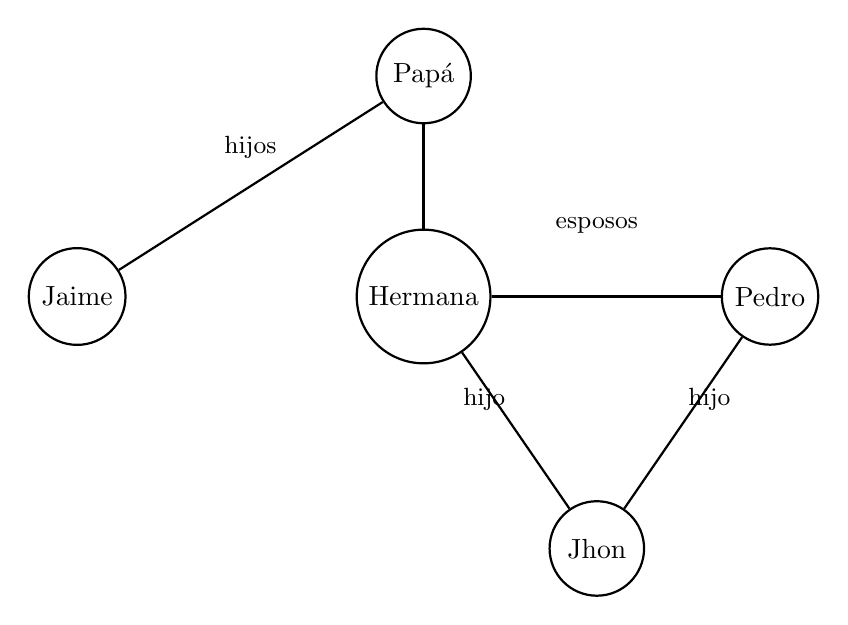
\begin{tikzpicture}[x=2.2cm,y=2cm]
		
		% Estilo de nodos
		\tikzset{
			persona/.style={
				circle,
				draw,
				thick,
				minimum size=1.2cm,
				align=center
			}
		}
		
		% Nodos
		\node[persona] (P) at (0,2) {Papá};
		\node[persona] (J) at (-2,0.6) {Jaime};
		\node[persona] (H) at (0,0.6) {Hermana};
		\node[persona] (Pe) at (2,0.6) {Pedro};
		\node[persona] (Jh) at (1,-1) {Jhon};
		
		% Líneas
		\draw[thick] (P) -- (J);
		\draw[thick] (P) -- (H);
		\draw[thick] (H) -- (Pe);
		\draw[thick] (H) -- (Jh);
		\draw[thick] (Pe) -- (Jh);
		
		% Etiquetas
		\node at (-1,1.55) {\small hijos};
		\node at (1,1.05) {\small esposos};
		\node at (0.35,-0.05) {\small hijo};
		\node at (1.65,-0.05) {\small hijo};
		
	\end{tikzpicture}
\end{center}


\vspace{6mm}
	
	\item Para ir de Puno a Juliaca hay 8 empresas de transporte y para ir de Juliaca a Huancané existen 5 empresas de transporte. ¿De cuántas maneras diferentes puede ir María de Puno a Huancané y regresar, pero en empresas de transporte diferentes?
	\begin{enumerate}[label=\alph*)]
		\item 560
		\item 800
		\item 1600
		\item 1120
		\item 1240
	\end{enumerate}
	\textbf{Respuesta correcta:} d)
	
	\vspace{2mm}
	\textbf{Solucionario:}\\
	De ida:
	
	$8 \times 5 = 40$\\
	
	De regreso, debe usar empresas diferentes en cada tramo:
	
	$7 \times 4 = 28$\\
	
	Entonces:
	
	$40 \times 28 = 1120$\\
	
	Por tanto, la cantidad total de maneras es \(\boxed{1120}\).
	
	\vspace{6mm}
	
	\item Tengo el doble de tu edad; pero él tiene el triple de la mía; si dentro de 6 años tu edad sumada a la mía será 18 años menos que la edad de él. ¿Qué edad tengo?
	\begin{enumerate}[label=\alph*)]
		\item 12
		\item 14
		\item 18
		\item 25
		\item 16
	\end{enumerate}
	\textbf{Respuesta correcta:} e)
	
	\vspace{2mm}
	\textbf{Solucionario:}\\
	Sea \(x\) tu edad. \\
	Mi edad es: $2x$\\
	y la edad de él: $3(2x)=6x$\\
	Dentro de 6 años:\\
	$(x+6)+(2x+6)=(6x+6)-18\\
	3x+12=6x-12\\
	24=3x\\
	x=8$\\
	Mi edad es:\\
	$2x=16\\
	$
	Por tanto, tengo \(\boxed{16}\) años.
	
	\vspace{6mm}
	
	\item Habiéndose declarado una epidemia en un rebaño de alpacas, murió el 12\% del total, quedando tan solo 2200 alpacas. ¿De cuántas alpacas constaba el rebaño?
	\begin{enumerate}[label=\alph*)]
		\item 2300
		\item 2350
		\item 2400
		\item 2450
		\item 2500
	\end{enumerate}
	\textbf{Respuesta correcta:} e)
	
	\vspace{2mm}
	\textbf{Solucionario:}\\
	Si murió el \(12\%\), quedó el \(88\%\) del total:

	$0.88T = 2200$\\
	$T = \frac{2200}{0.88}=2500$\\
	Entonces, el rebaño constaba de \(\boxed{2500}\) alpacas.
	
	\vspace{6mm}
	
	\item La mitad del tiempo transcurrido desde las 8:00 hrs. es igual a la sexta parte de lo que falta transcurrir para terminar el día. ¿Qué hora es?
	\begin{enumerate}[label=\alph*)]
		\item 04:00 hrs.
		\item 06:00 hrs.
		\item 10:00 hrs.
		\item 08:00 hrs.
		\item 12:00 hrs.
	\end{enumerate}
	\textbf{Respuesta correcta:} e)
	
	\vspace{2mm}
	\textbf{Solucionario:}\\
	Sea \(t\) el número de horas transcurridas desde las 8:00.\\
	Entonces:

	$\dfrac{t}{2}=\frac{16-t}{6}\\
	3t = 16 - t\\
	4t = 16\\
	t=4$\\
	Entonces han pasado 4 horas desde las 8:00:
	8:00 + 4 = 12:00

	La hora es \(\boxed{12:00\ \text{hrs.}}\)
	
	\vspace{6mm}
	
\end{enumerate}

\subsection*{Razonamiento Verbal}

\begin{enumerate}
	
	\item El antónimo de la palabra PERVERSO es:
	\begin{enumerate}[label=\alph*)]
		\item infame.
		\item virtuoso.
		\item atroz.
		\item inicuo.
		\item inepto.
	\end{enumerate}
	\textbf{Respuesta correcta:} b)
	
	\vspace{2mm}
	\textbf{Solucionario:}\\
	\textbf{Perverso} significa malvado o depravado. Su antónimo es \textbf{virtuoso}, que alude a una persona moralmente buena.
	
	\vspace{6mm}
	
	\item La raíz latina de HUMO es:
	\begin{enumerate}[label=\alph*)]
		\item fumus.
		\item humus.
		\item homo.
		\item hemi.
		\item motus.
	\end{enumerate}
	\textbf{Respuesta correcta:} a)
	
	\vspace{2mm}
	\textbf{Solucionario:}\\
	La palabra \textbf{humo} proviene del latín \textbf{fumus}, que significa precisamente humo.\\
	Por eso, la alternativa correcta es \textbf{a) fumus}..
	
	\vspace{6mm}
	
	\item Aquí vemos, entre los iroqueses y entre los griegos, el primer \textbf{Germen} de familias nobles.\\
	El sinónimo de la palabra resaltada es:
	\begin{enumerate}[label=\alph*)]
		\item compuesto.
		\item hijo.
		\item vástago.
		\item origen.
		\item producto.
	\end{enumerate}
	\textbf{Respuesta correcta:} d)
	
	\vspace{2mm}
	\textbf{Solucionario:}\\
	En el contexto de la oración, \textbf{germen} significa inicio, principio o \textbf{origen}. Por ello, la respuesta correcta es \textbf{origen}.
	
	\vspace{6mm}
	
	\item Identifique el vicio de dicción que se comete en el enunciado:\\
	``En mi vida ajetreada, donde las responsabilidades y el estrés son una constante, a veces anhelo simplemente desconectar y encontrar un rincón donde pueda disfrutar de la tranquilidad de que quiero quedarme quieto, lejos del bullicio del mundo exterior.''
	\begin{enumerate}[label=\alph*)]
		\item Queísmo
		\item Vulgarismo
		\item Pleonasmo
		\item Cacofonía
		\item Extranjerismo
	\end{enumerate}
	\textbf{Respuesta correcta:} d)
	
	\vspace{2mm}
	\textbf{Solucionario:}\\
	En el enunciado se percibe repetición desagradable de sonidos, especialmente en secuencias como \textit{que quiero quedarme quieto}. Ese defecto de expresión recibe el nombre de \textbf{cacofonía}.
	
	\vspace{6mm}
	
	\item Resuelva el par analógico:\\
	JACTANCIOSO : VANIDOSO ::
	\begin{enumerate}[label=\alph*)]
		\item presuntuoso : engreído.
		\item soberbio : humilde.
		\item arrogante : apocado.
		\item tímido : inseguro.
		\item simpático : afable.
	\end{enumerate}
	\textbf{Respuesta correcta:} a)
	
	\vspace{2mm}
	\textbf{Solucionario:}\\
	\textbf{Jactancioso} y \textbf{vanidoso} mantienen relación de sinonimia. La alternativa que conserva esa misma relación es \textbf{presuntuoso : engreído}.
	
	\vspace{6mm}
	
	\item \textbf{Comprensión de lectura}\\
	El hombre común puede vivir sin recordar de memoria muchos hechos, pero algunos son indispensables: el descubrimiento de América, el día de nuestra independencia, la fecha de cumpleaños de la esposa, el año y día de su casamiento.\\
	Según el párrafo, ¿quién puede padecer del recordar?
	\begin{enumerate}[label=\alph*)]
		\item El psicópata
		\item El ignorante
		\item El que es cretino
		\item El atacado de catalepsia
		\item El que sufre de amnesia
	\end{enumerate}
	\textbf{Respuesta correcta:} e)
	
	\vspace{2mm}
	\textbf{Solucionario:}\\
	El texto trata sobre la capacidad de recordar hechos importantes. La persona que padece una alteración directamente relacionada con la memoria es quien sufre de \textbf{amnesia}. Por eso, esa es la respuesta correcta.
	
	\vspace{6mm}
	
\end{enumerate}

\subsection*{Inglés}

\begin{enumerate}
	
	\item Look at the picture, describe and answer this question.\\
	\textit{What was she doing?}
	
	\begin{center}
		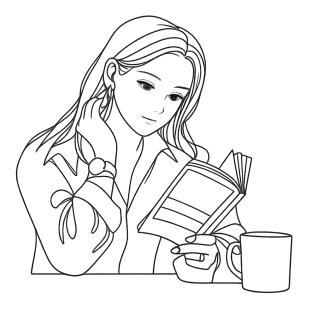
\includegraphics[width=3.5cm]{imagenes/CEPRE-UNA2024-I/etapa1/soc/ingles1c24-I.png}
	\end{center}
	
	\begin{enumerate}[label=\alph*)]
		\item She was dancing.
		\item She was reading.
		\item She was sleeping in her bed.
		\item She was watching TV.
		\item She was swimming.
	\end{enumerate}
	\textbf{Respuesta correcta:} b)
	
	\vspace{2mm}
	\textbf{Solucionario:}\\
	En la imagen se observa a  . Por ello, la descripción correcta es: \textbf{She was reading.}
	
	\vspace{6mm}
	
	\item Complete the sentences with the correct prepositions.\\
	\textit{Peru anniversary is \_\_\_\_ July \_\_\_\_ the 28th.}
	\begin{enumerate}[label=\alph*)]
		\item in -- at
		\item on -- on
		\item on -- in
		\item in -- on
		\item in -- in
	\end{enumerate}
	\textbf{Respuesta correcta:} d)
	
	\vspace{2mm}
	\textbf{Solucionario:}\\
	En inglés se usa \textbf{in} para meses y \textbf{on} para fechas específicas.\\
	Por tanto:
	\[
	\textit{Peru anniversary is in July on the 28th.}
	\]
	La respuesta correcta es \textbf{in -- on}.
	
	\vspace{6mm}
	
\end{enumerate}

\subsection*{Quechua y Aimara}

\begin{enumerate}
	
	\item ¿Imamantaq yachaqkunari kuraq yachay wasita rinku? / ¿Kunarusa yatiqirinakaxa jach'a yatiqaña utaru sarapxi?
	\begin{enumerate}[label=\alph*)]
		\item Tusuq / Thuquri
		\item Pukllaq / Anatiri
		\item Yachaq / Yatiqañataki
		\item Mikhumuq / Manq'iri
		\item Puriquq / Sarnaqiri
	\end{enumerate}
	\textbf{Respuesta correcta:} c)
	
	\vspace{2mm}
	\textbf{Solucionario:}\\
	La pregunta se relaciona con el estudio o el aprendizaje en una institución mayor de enseñanza. La alternativa que corresponde semánticamente a esa idea es \textbf{Yachaq / Yatiqañataki}.
	
	\vspace{6mm}
	
	\item ¿Mayqantaq wasi uywari? / ¿Kawkirisa uta uywaxa?
	\begin{enumerate}[label=\alph*)]
		\item Taruka / Taruka
		\item Misi / Phisi
		\item Atuq / Qamaqi
		\item Añas / Añuthaya
		\item Anka / Allqamari
	\end{enumerate}
	\textbf{Respuesta correcta:} b)
	
	\vspace{2mm}
	\textbf{Solucionario:}\\
	La pregunta hace referencia al animal doméstico o criado en casa. Entre las alternativas, \textbf{misi / phisi} corresponde al \textbf{gato}, que es un animal doméstico. Por ello, esa es la respuesta correcta.
	
	\vspace{6mm}
	
\end{enumerate}






